\documentclass[12pt,a4paper]{article}

\usepackage[onehalfspacing]{setspace}
 
\usepackage{float}
%f�r feststellen der figures und tables [H] dranschreiben
\usepackage{siunitx}
%\SI{value}{unit commands} \SI{value}[pre-unit]{unit commands}
%\usepackage{units}
%wird so benutzt: 
%\unit[value/Zahl]{dimension/Einheit} oder 
%\unitfrac[value/Zahl]{dimension/Einheit num/Z�hler}{dimension/Einheit denum/Nenner} oder
%\nicefrac[fontcommand/Schriftart]{dimension/Einheit num/Z�hler}{dimension/Einheit denum/Nenner}
\usepackage{amssymb}
\usepackage{caption}
\usepackage{subcaption}

\usepackage{hyperref}

\usepackage[left=2cm,right=2cm,top=2cm,bottom=2cm]{geometry}
\usepackage[latin9]{inputenc}
\usepackage[ngerman]{babel}
\usepackage[T1]{fontenc}
\usepackage{lmodern}
\usepackage{amsmath}
\usepackage{graphicx}
\usepackage{textcomp}

\usepackage[style=numeric,sorting=nyt,firstinits=true,backend=bibtex]{biblatex}
\usepackage[babel,german=guillemets]{csquotes}
\bibliography{ref.bib}


\begin{document}

%deckblatt erstellen.

\begin{titlepage}

\begin{center}
% Oberer Teil der Titelseite:

\includegraphics[width=0.75\textwidth]{logo.png}\\[1cm]    	%Logo 

\textsc{\LARGE Bergische Universit\"at Wuppertal}\\[1.5cm]	%Institution

\textsc{\Large Fortgeschrittenen Praktikum}\\[0.5cm]				%Projekt


\newcommand{\HRule}{\rule{\linewidth}{0.5mm}}
\HRule \\[0.4cm]
{ \huge \bfseries Rutherford\\ Streuung von $\alpha$-Teilchen}\\[0.4cm]				%Titel

\HRule \\[1.5cm]

% Author und Tutor
\begin{minipage}{0.4\textwidth}
\begin{flushleft} \large
\emph{Verfasser:}\\
Henrik \textsc{J�rgens} \\
Frederik \textsc{Strothmann} \\
\end{flushleft}
\end{minipage}
\hfill
\begin{minipage}{0.4\textwidth}
\begin{flushright} \large
\emph{Tutoren:} \\
Max \textsc{Mustermann} \\
Max \textsc{Mustermann} \\
\end{flushright}
\end{minipage}

\vspace{1cm}

\begin{table}[H]
\centering
\begin{tabular}{|l|}
\hline \textbf{Abstract: } \\
Ziel des Versuches ist es, die Wechselwirkung von $\alpha$-Teilchen mit Materie zu untersuchen.\\
Die Aspekte Streuwinkel, Reichweite, Kernladung und Absorbtionsverhalten werden thematisiert.\\
\hline 
\end{tabular}
\end{table} 

\vspace{1cm}

\begin{table}[H]
\centering
\begin{tabular}{|c|c|c|}
\hline Dies & ist & ein \\ 
\hline Platz- & halter & f�r \\ 
\hline die & bewertungs & Tabelle \\ 
\hline 
\end{tabular} 
\end{table}

\vfill

% Unterer Teil der Seite/Datum
{\large \today}

\end{center}

\end{titlepage}

\newpage
\tableofcontents
\newpage


\section{Einleitung}
%einleitung zu dem experiment.
%auf die einstellungen, die vor dem versuch gemacht werden, eingehen, oder auf eine anleitung dazu verweisen.
%---------------------------------------------------------------------------------------------
%hinter der einleitung kann der allgemeine theoretische hintergrund in einer zus�tzlichen section erkl�rt werden
In diesem Versuch werden Oberfl�chen verschiedener Proben mittels Rasttunnelmikroskopie auf deren Gitterstruktur und morphologische Eigenschaften untersucht. Elektronendichte, Oberfl�chenrauheit und die atomare Gitterstruktur k�nnen mit dem Rastertunnelmikroskop (RTM) analysiert werden. Der quantenmechanische Tunneleffekt wird genutzt, um leitende Materialien zu untersuchen. Indem zwischen einer einatomigen Platin-Iridum-Elektrode und der zu untersuchenden Probe eine Potentialdifferenz angelegt wird, kommt es abh�ngig von der Entfernung der Pt-Ir-Elektrode zur Probe und dessen Elektronendichte zu einem Tunnelstrom, welcher R�ckschl�sse auf die Struktur der Probe erlaubt. Die Elektronendichte der Oberfl�che kann durch systematisches Abrastern der Probe erfasst werden, sodass mithilfe verschiedener Modi (CC und CH: Constant Current und Constant Height) ein Bild der Materialoberfl�che entsteht.
\section{Theorie}
% Es sollen die wichtigsten theoretischen Formeln und Zusammenh�nge einmal ausf�hrlich erkl�rt werden
Es werden die theoretischen Grundlagen zur Bestimmung der Lebensdauer von Myonen besprochen.

\subsection{Standardmodell}
Das Standartmodell der Teilchenphysik drei der vier Grundlegenden Wechselwirkungen (WW), die schwache WW, die elektromagnetische WW und die Starke WW.
Die Kr�fte wechselwirken �ber Vektorbosonen, welche eine ganzzahligen Spin haben.
In Tabelle \ref{tab:ww} ist eine �bersicht der drei Kr�fte zu sehen.

\begin{table}[H]
\caption{In der Tabelle sind die Grundlegenden WW (au�er der Gravitation) und ihre Eigenschaften aufgetragen (entnommen \cite{povh} Seite 274)}
\label{tab:ww}
\centering
\begin{tabular}{|c|c|c|c|c|}
\hline Wechselwirkung & koppelt an & Austauschteilchen & $\frac{m_0}{GeV}$ & J$^P$ \\ 
\hline stark & Farbe & 8 Gluonen (g) & 0 & 1$^-$ \\ 
\hline elektromagnetisch & elektrische Ladung & Photon ($\gamma$) & 0 & 1$^-$ \\ 
\hline schwach & schwache Ladung & W$^\pm$, Z$^0$ & $\approx 10^2$ & 1 \\ 
\hline 
\end{tabular} 
\end{table}
Neben den Bosonen gibt es noch zwei weitere Fundamentale Teilchenarten die Quark und die Leptonen welche die Grundbausteine der Materie darstellen.
Beide geh�ren zu den Fermionen, haben also einen halbzahligen Spin. Leptonen und Quarks werden mit aufsteigender Masse in drei Generationen aufgeteilt.
In Tabelle \ref{tab:fermi} sind Quarks und Leptonen mit ihren Eigenschaften dargestellt.

\begin{table}[H]
\caption{�bersicht der Grundlegenden Eigenschaften von Quarks und Leptonen}
\label{tab:fermi}
\centering
\begin{tabular}{|p{2cm}|p{2cm}|p{2cm}|p{1cm}|p{3.5cm}|p{1cm}|}
	\hline
	Fermionen & \hspace{0.25cm} Familie \newline 1 \hspace{0.3cm} 2 \hspace{0.3cm} 3                                               & elektrische Ladung    & Farbe  & schwacher Isospin \newline rechtsh. \hspace{0.5cm} linksh. & Spin \\ \hline
	Leptonen  & $\nu_e$ \hspace{0.17cm} $\nu_\mu$ \hspace{0.17cm} $\nu_\tau$ \newline e \hspace{0.3cm} $\mu$ \hspace{0.3cm} $\tau$ & \hspace{0.6cm} 0 \newline  \hspace*{0.6cm} -1      & ------ & 1/2 \hspace{1.5cm} --- \newline \hspace*{2.4cm} 0          & 1/2  \\ \hline
	Quarks    & u \hspace{0.3cm} c \hspace{0.3cm} t \newline d \hspace{0.3cm} s \hspace{0.3cm} b                                   & \hspace*{0.2cm} +2/3 \newline \hspace*{0.3cm} -1/3 & r,g,b  & 1/2 \hspace{1.64cm} 0 \newline \hspace*{2.4cm} 0           & 1/2  \\ \hline
\end{tabular} 
\end{table}


\section{Versuchsaufbau}
%skizze zum versuchsaufbau (oder foto) einf�gen,   es muss erkl�rt werden wie das ganze funktioniert und welche speziellen einstellungen verwendet wurden (z.b. welche kn�pfe an den ger�ten f�r die messung verdreht wurden)
F�r den Versuch werden zwei verscheiden Vakuumkammern verwendet. Die erste Kammer  ist eine Rutherford-Streukammer, eine schematische Skizze ist in Abb. \ref{fig:kammer} zu sehen. Die Streukammer besteht aus einer Vakuumkammer, mit durchsichtigem Deckel. Ein Barometer, ein Bel�ftungsventil und ein Ventil mit Anschluss an die Vakuumpumpe sind an den Absperrhahn (3) angeschlossen. Der Halbleiterdetektor mit Kollimator (12,12.1) ist von innen an einer BNC-Buchse (2.1) montiert. Von au�en ist ein Vorverst�rker angeschlossen, die Daten werden von einem Digitalz�hler, der an einen Computer angeschlossen ist ausgelesen (siehe Abb. \ref{fig:aufbau}). Der Deckel der Streukammer hat einen Schwenkarm (7), an dem das $^{241}$Am-Pr�parat (7.1) , verschiedene Rahmen mit SpaltkKollimatoren (9) und Metallfolien (10) angebracht werden k�nnen. �ber einen Knopf (4) ist der Schwenkarm drehbar, der Winkel ist dabei �ber eine Skala (8) ablesbar. Zur Verf�gung stehen Spalte mit 1m und 5mm Breite sowie eine Goldfolie mit 2$\mu$m und eine Aluiminiumfolie mit 7$\mu$m Dicke.

\begin{figure}[H]
	\centering
  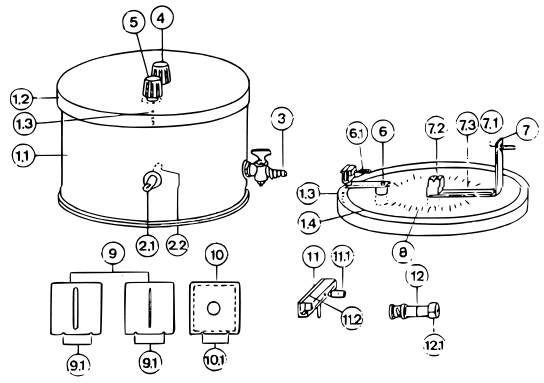
\includegraphics[scale=0.4]{streukammer.png}
	\caption{Schematischer Aufbau des Streukammer}
	\label{fig:kammer}
\end{figure}


\begin{figure}[H]
	\centering
  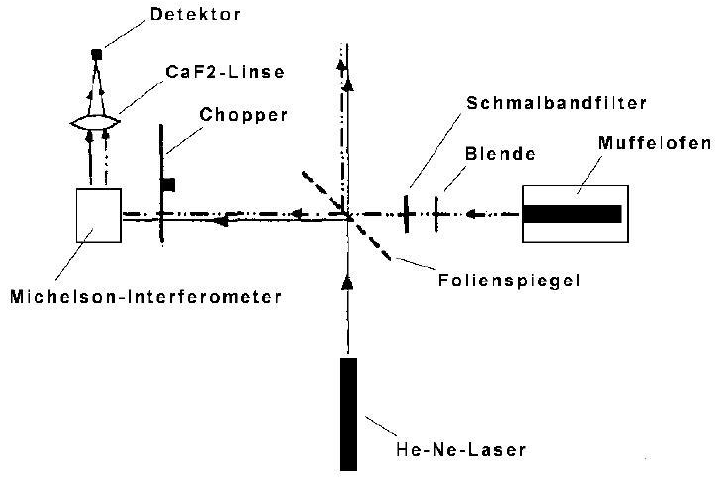
\includegraphics[scale=0.4]{aufbau.png}
	\caption{Schematischer Aufbau des Versuchsaufbaus}
	\label{fig:aufbau}
\end{figure}

Die zweite Kammer ist eine Vakuumkammer, mit einer optischen Bank, zu befestigen der radioaktiven Quelle. Sie wird f�r die Bestimmung der Reichweite von $\alpha$-Strahlung und die Untersuchung von Absorbtion durch verschiedenen Medien verwendet. Der Detektor ist an einen PC angeschlossen mit dem die Messdaten aufgenommen werden.
\section{Detektorspannung in Abh�ngigkeit der Chopperfrequenz}

Zu erste soll die der Zusammenhang zwischen der Detektorspannung U und der Chopperfrequenz f untersucht werden. Die Chopperfrequenz wird im Bereich von 20Hz bis 50Hz variiert. Bei Werten unter 20Hz ist die Schwankung der Werte zu gro�, so dass die Signale nicht vom Untergrund unterschieden werden k�nnen. Die Detektorspannung wird am Log-In-Verst�rker abgelesen, dabei wurde ein Fehler von ?? V angenommen, da die Anzeige in diesem Bereich schwankte. Der Plot der Messdaten mit linearen Achsen ist in Abbildung ?? zu sehen. In Abbildung ?? sind die Messdaten mit doppelt logarithmischen Achsen geplotted. Da ein linearer Zusammenhang zwischen log(U) und log(f) zu sehen ist, werden die Messdaten mit  Gleichung ?? gefitted.

\begin{align}
U(f) = exp[A \cdot log(f) + B]
\end{align}

Dabei sind A und B freie Parameter, die durch den Fit bestimmt werden. Das Ergebnis des Fits ist in Tabelle ?? zu sehen.

\subsection{Kalibrierung und Bestimmung der Wellenl�nge des Lasers}
In diesem Abschnitt soll das �bersetzungsverh�ltnis zwischen Schraube und Spiegel und die Wellenl�nge des Lasers bestimmt werden. Zuvor muss noch die x-Position in Lab-View und der Millimeterschraube geeicht werden.

\subsubsection{Kalibrierung}
\label{Eichung}
Die x-Werte in Lab-View m�ssen den realen Positionen der Millimeterschraube zugeordnet werden. Bei der Bestimmung wird von einem linearem Zusammenhang ausgegangen. F�r die Kalibrierung wird die Schraube gedreht, dabei wird in regelm��igen Abst�nden die Position im Interferogramm mit Lab-View aufgenommen. Der Fehler der Schraubenposition wird mit 5$\mu$m angenommen (eine halbe Skaleneinheit). F�r den Fit wurde Gleichung \ref{eqn:lin_fit} verwendet, A beschreibt dabei die Steigung und B das Offset. Der ist in Abbildung \ref{fig:eichung_laser} zu sehen. Aus dem Fit ergebe sich die Parameter in Tabelle \ref{tab:eichung_laser}.
\begin{align}
\label{eqn:lin_fit}
S(x) = A \cdot x + B
\end{align}

\begin{figure}[H]
\centering
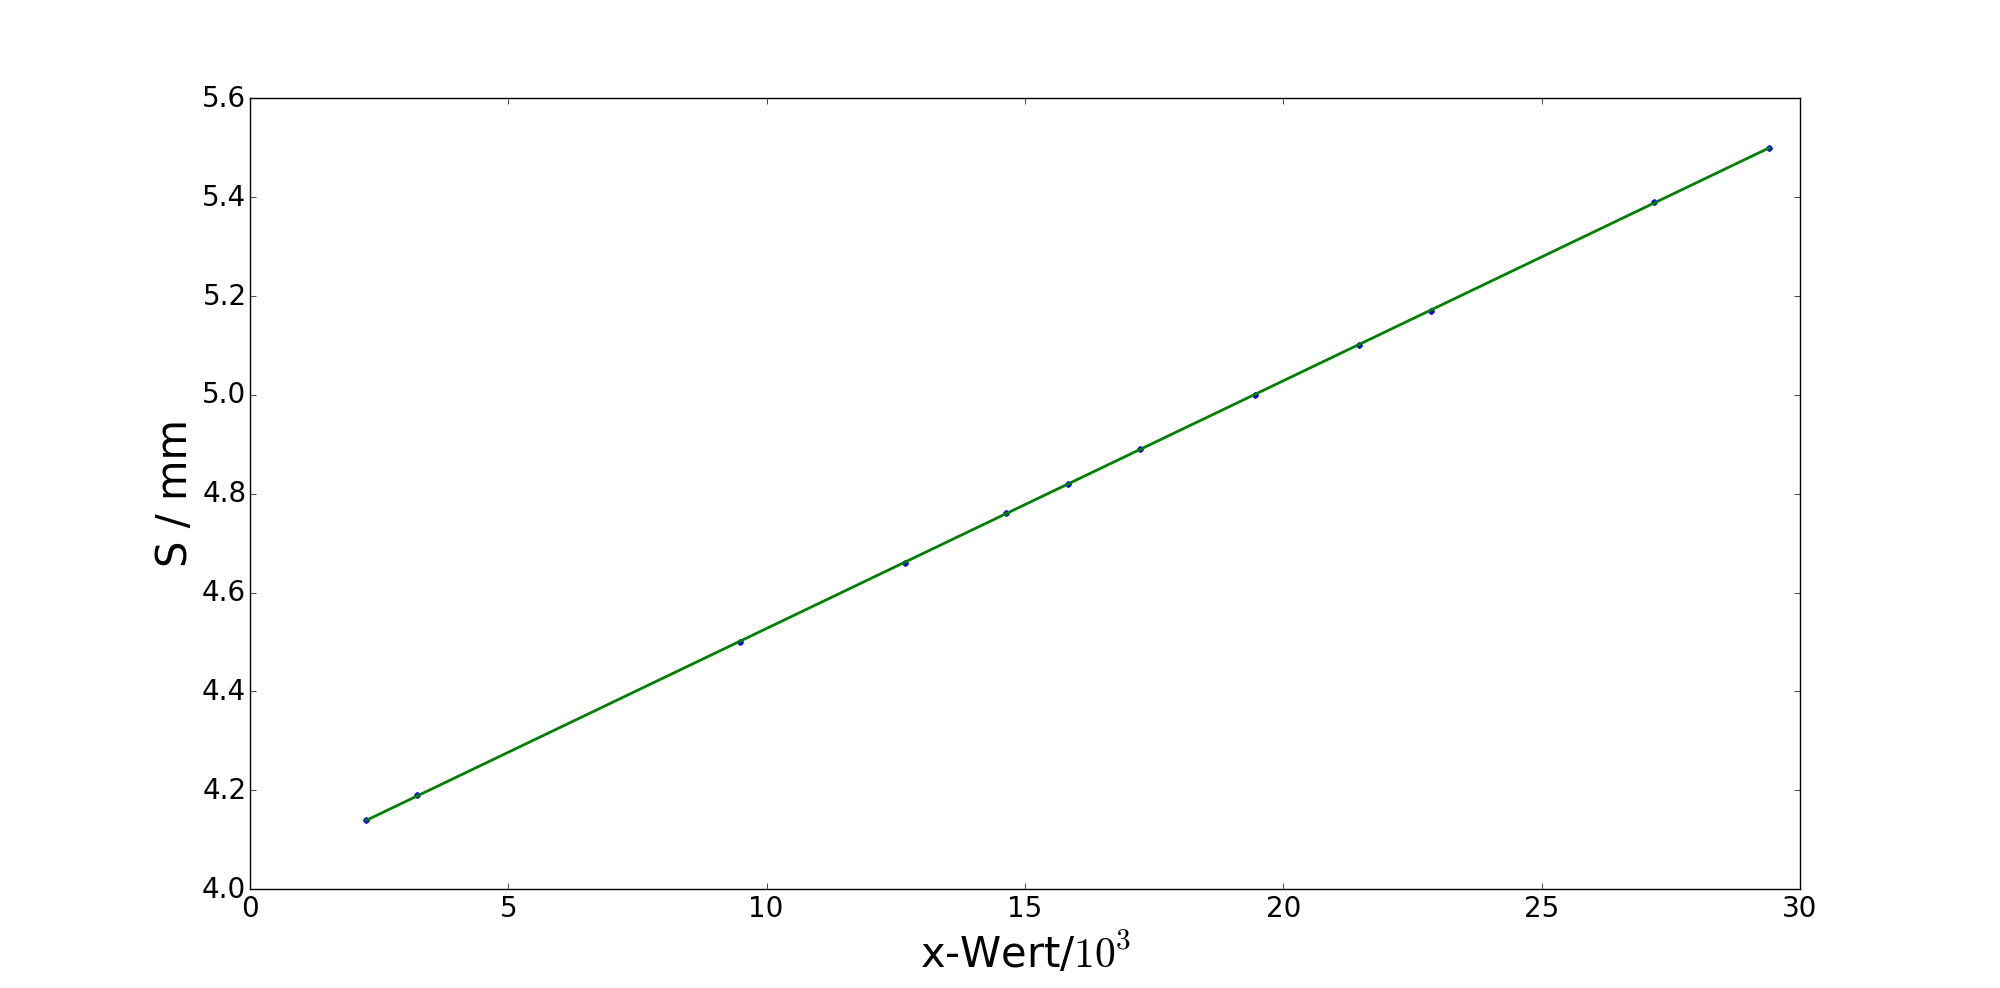
\includegraphics[scale = 0.33]{eichung_laser.png}
\caption{Linearer Fit f�r den Zusammenhang zwischen Kanal in Lab-View und der Position der Millimeterschraube. Die Fehler der Messpunkte sind so klein, dass sie nicht zu erkennen sind.}
\label{fig:eichung_laser}
\end{figure}

\begin{table}[H]
\centering
\caption{Parameter aus dem Fit f�r den Zusammenhang zwischen Kanal in Lab-View und der Position der Millimeterschraube}
\label{tab:eichung_laser}
\begin{tabular}{|c|c|}
\hline Parameter & Wert \\ 
\hline A / mm & 5.009(8)e-05 \\ 
\hline B / mm & 4.0263(9) \\ 
\hline $\chi_{red}^2$ & 0.78 \\ 
\hline 
\end{tabular} 
\end{table}

\subsection{Bestimmung der Wellenl�nge des Lasers}
Mit der zuvor durchgef�hrten Kalibrierung kann nun die Wellenl�nge $\lambda$ des Lasers bestimmt werden. Die Wellenl�nge wird aus dem Gangunterschied s, der Anzahl der Interferenzmaxima n und dem �bersetzungsverh�ltnis k bestimmt. F�r das �bersetzungsverh�ltnis wird ein Wert von k=5 angenommen. Die Wellenl�nge ergibt sich nach Gleichung \ref{eqn:wellenlaenge}.

\begin{align}
\label{eqn:wellenlaenge}
\lambda = \frac{2s}{kn}
\end{align}

Das aufgenommen Interferogramm ist in Abbildung \ref{fig:laser} zu sehen.

\begin{figure}[H]
\centering
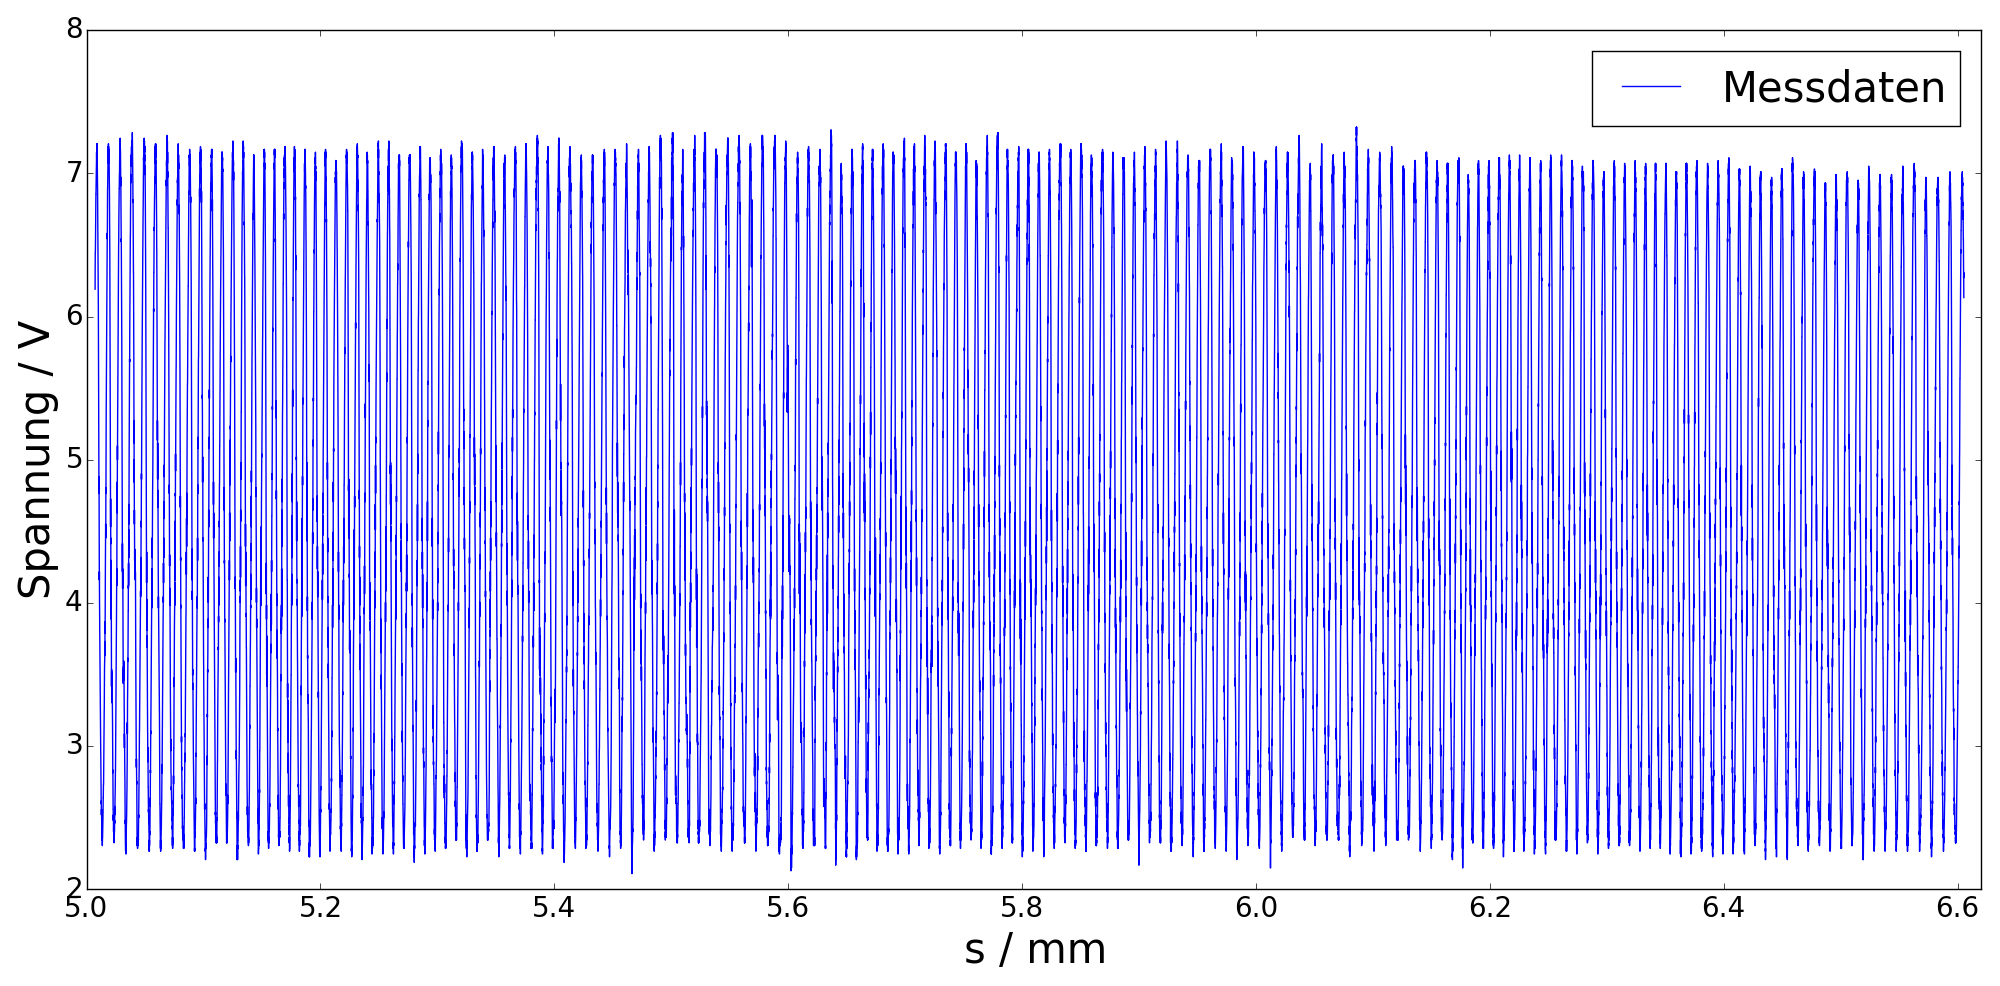
\includegraphics[scale = 0.33]{laser_interferogram.png}
\caption{Interferogramm des Lasers. Es wurden 173 Peaks aufgenommen}
\label{fig:laser}
\end{figure}

Mit der zuvor durchgef�hrten Kalibrierung wird der Gangunterschied der x-Position in eine reelle Wegdifferenz umgerechnet, der Fehler ergibt sich nach Fehlerfortpflanzung auf die Geradengleichung. Die Anzahl der Maxima wurde als Fehlerlos angenommen. Die Messdaten sind in Tabelle \ref{tab:wellenlaenge} eingetragen. Aus den bestimmten Wellenl�ngen ergibt sich ein Mittelwert von 3.732(9) $\mu$m. 

\begin{table}
\centering
\caption{Messergebnisse f�r die Bestimmung der Wellenl�nge}
\label{tab:wellenlaenge}
\begin{tabular}{|c|c|c|c|c|}
\hline n & s$_1$ / mm & s$_2$ / mm & $\Delta$s / mm & $\lambda$ / $\mu$m \\ 
\hline 173 & 5.0088(3) & 6.6040(3) & 1.5952(4) & 3.688(9) \\ 
\hline 172 & 5.0107(3) & 6.6040(3) & 1.5933(4) & 3.705(9) \\ 
\hline 171 & 5.0127(3) & 6.6040(3) & 1.5913(4) & 3.722(9) \\ 
\hline 170 & 5.0151(3) & 6.6040(3) & 1.5889(4) & 3.738(9) \\ 
\hline 169 & 5.0493(3) & 6.6040(3) & 1.5547(4) & 3.739(9) \\ 
\hline 168 & 5.0589(3) & 6.6040(3) & 1.5451(4) & 3.742(9) \\ 
\hline 167 & 5.0689(3) & 6.6040(3) & 1.5351(4) & 3.743(9) \\ 
\hline 166 & 5.0784(3) & 6.6040(3) & 1.5256(4) & 3.746(9) \\ 
\hline 165 & 5.0884(3) & 6.6040(3) & 1.5159(4) & 3.746(9) \\ 
\hline 164 & 5.0975(3) & 6.6040(3) & 1.5600(4) & 3.752(9) \\ 
\hline 
\end{tabular} 
\end{table}


Um ein besseres Ergebnis zu erhalten, wird das eigentliche �bersetzungsverh�ltnis $k_e$ mit Gleichung \ref{eqn:uebersetzungsverhaeltniss} bestimmt. Dabei wurde f�r $\lambda$ der Literaturwert von 3,39$\mu$m verwendet (vgl. \ref{eqn:uebersetzungsverhaeltniss}). Der korrigierte �bersetzungsfaktor ergibt sich mit 5.42(1). In den nachfolgenden Versuchsteilen wird das korrigierte �bersetzungsverh�ltnis verwendet.

\begin{align}
\label{eqn:uebersetzungsverhaeltniss}
k_e = \frac{2s}{n\lambda}
\end{align}
\subsection{Bestimmung der Wei�lichtpositon der polychromatischen Strahlung des Muffelofen}
Bei wei�em Licht gibt es nur an der Wei�lichtposition konstruktive Interferenz, da an dieser Positon der Gangunterschied gleich 0 ist. Die Wei�lichtposition des Muffelofen liegt also in Abh�ngigkeit der Spiegelpostion dort, wo die Intensit�t maximal wird. Neben der Wei�lichtposition kann von einer Gleichverteilung zwischen konstruktiver- und destruktiver Interferenz ausgegangen werden. Bei der Suche nach dem Wei�lichtpunkt wurden zwei Kandidaten gefunden. 

Der erste Wei�lichtpunkt wurde bei 4,7545(80) mm gefunden, siehe Abbildung \ref{fig:weisslichtpunkt_1}. Der zweite Wei�lichtpunkt wurde bei  5,770(3) mm gefunden, sieh Abbildung \ref{fig:weisslichtpunkt_2}. Die Herkunft des zweiten Wei�lichtpunktes ist nicht bekannt.

\begin{figure}[H]
\centering
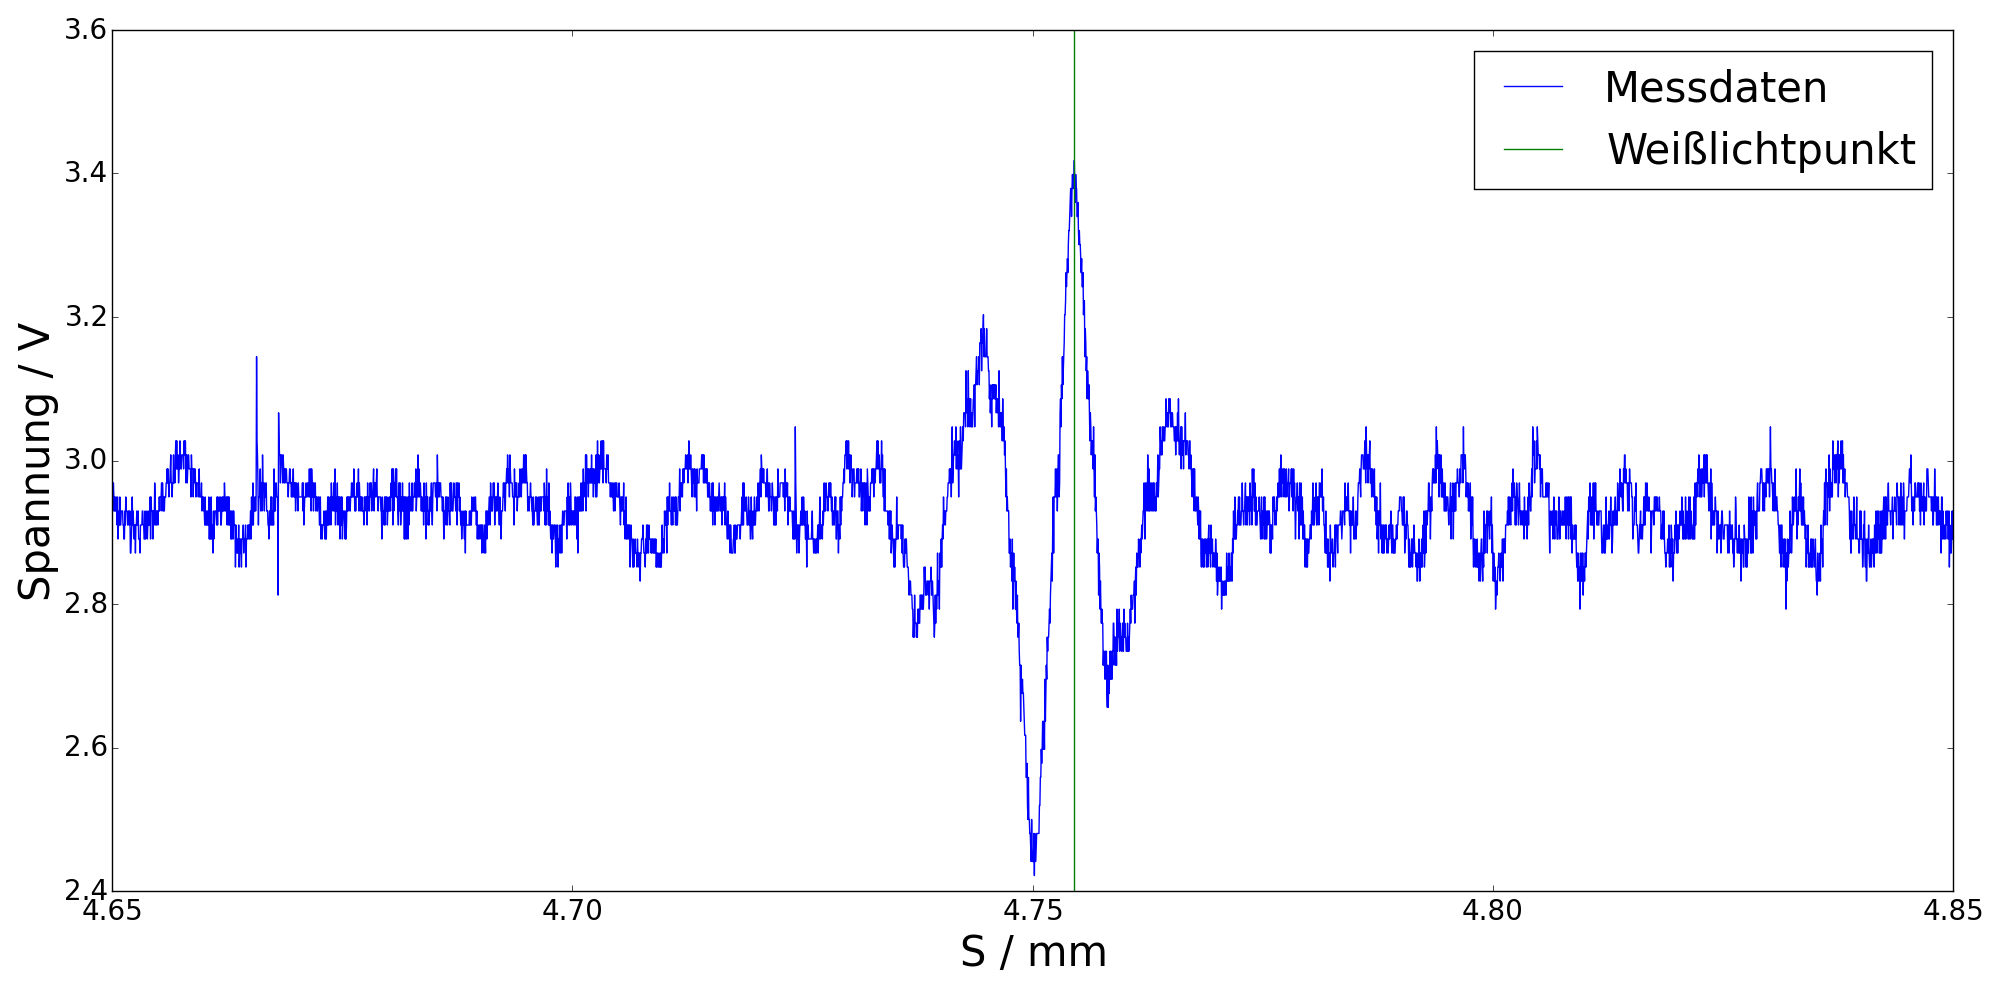
\includegraphics[scale = 0.33]{weisslichtpunkt_4,77.png}
\caption{Erster bestimmter Wei�punkt bei 4,755(8) mm}
\label{fig:weisslichtpunkt_1}
\end{figure}

\begin{figure}[H]
\centering
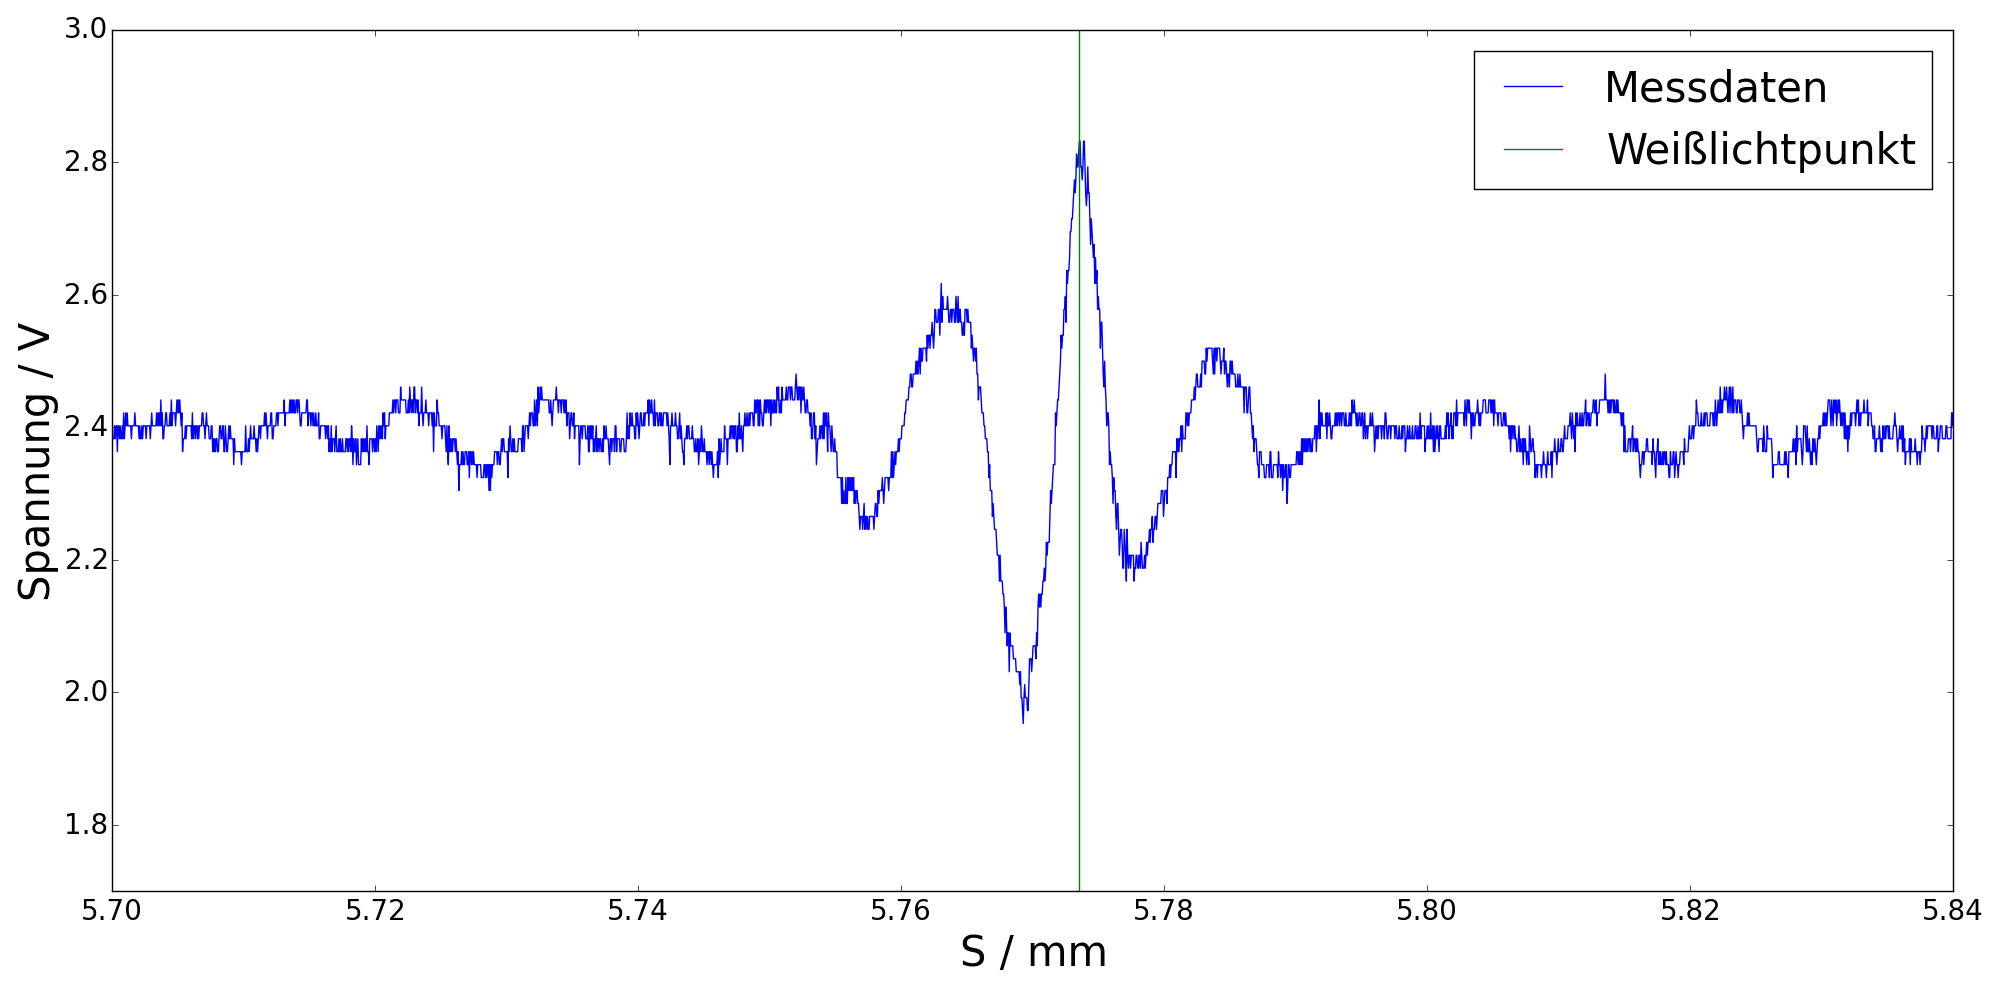
\includegraphics[scale = 0.33]{weisslichtpunkt_5,8.png}
\caption{Zweiter bestimmter Wei�punkt bei 5,770(3) mm}
\label{fig:weisslichtpunkt_2}
\end{figure}

Die beiden Plots, f�r die Eichung des Abstandes und die Tabellen mit den Parametern sind im Anhang in Abschnitt \ref{subsec:weisslicht} zu finden.
\section{Analyse des Schmalbandinterferogramms}
\label{sec:filter}
Der Wellenl�ngenbereich des Muffelofen wird mit einem Schmalbandfilter reduziert. Da durch die Filterung auch die Intensit�t verringert wird, muss die Verst�rkung des Log-In-Verst�rkers korrigiert werden. Aufgrund des Filters wird eine ged�mpfte Cosinus-Schwingung symmetrisch um den Wei�lichtpunkt des Muffelofen erwartet. Aus dem aufgenommen Interferogramm soll die Wellenl�nge der maximalen Transmission und die Breite des 1/e-Abfalls der Einh�llenden bestimmt werden. Mit diesen beiden Werten kann die Breite des Schmalbandfilters bestimmt werden.
Das Interferogramm ist in Abbildung \ref{fig:filter_weiss} zu sehen. 

\begin{figure}[H]
\centering
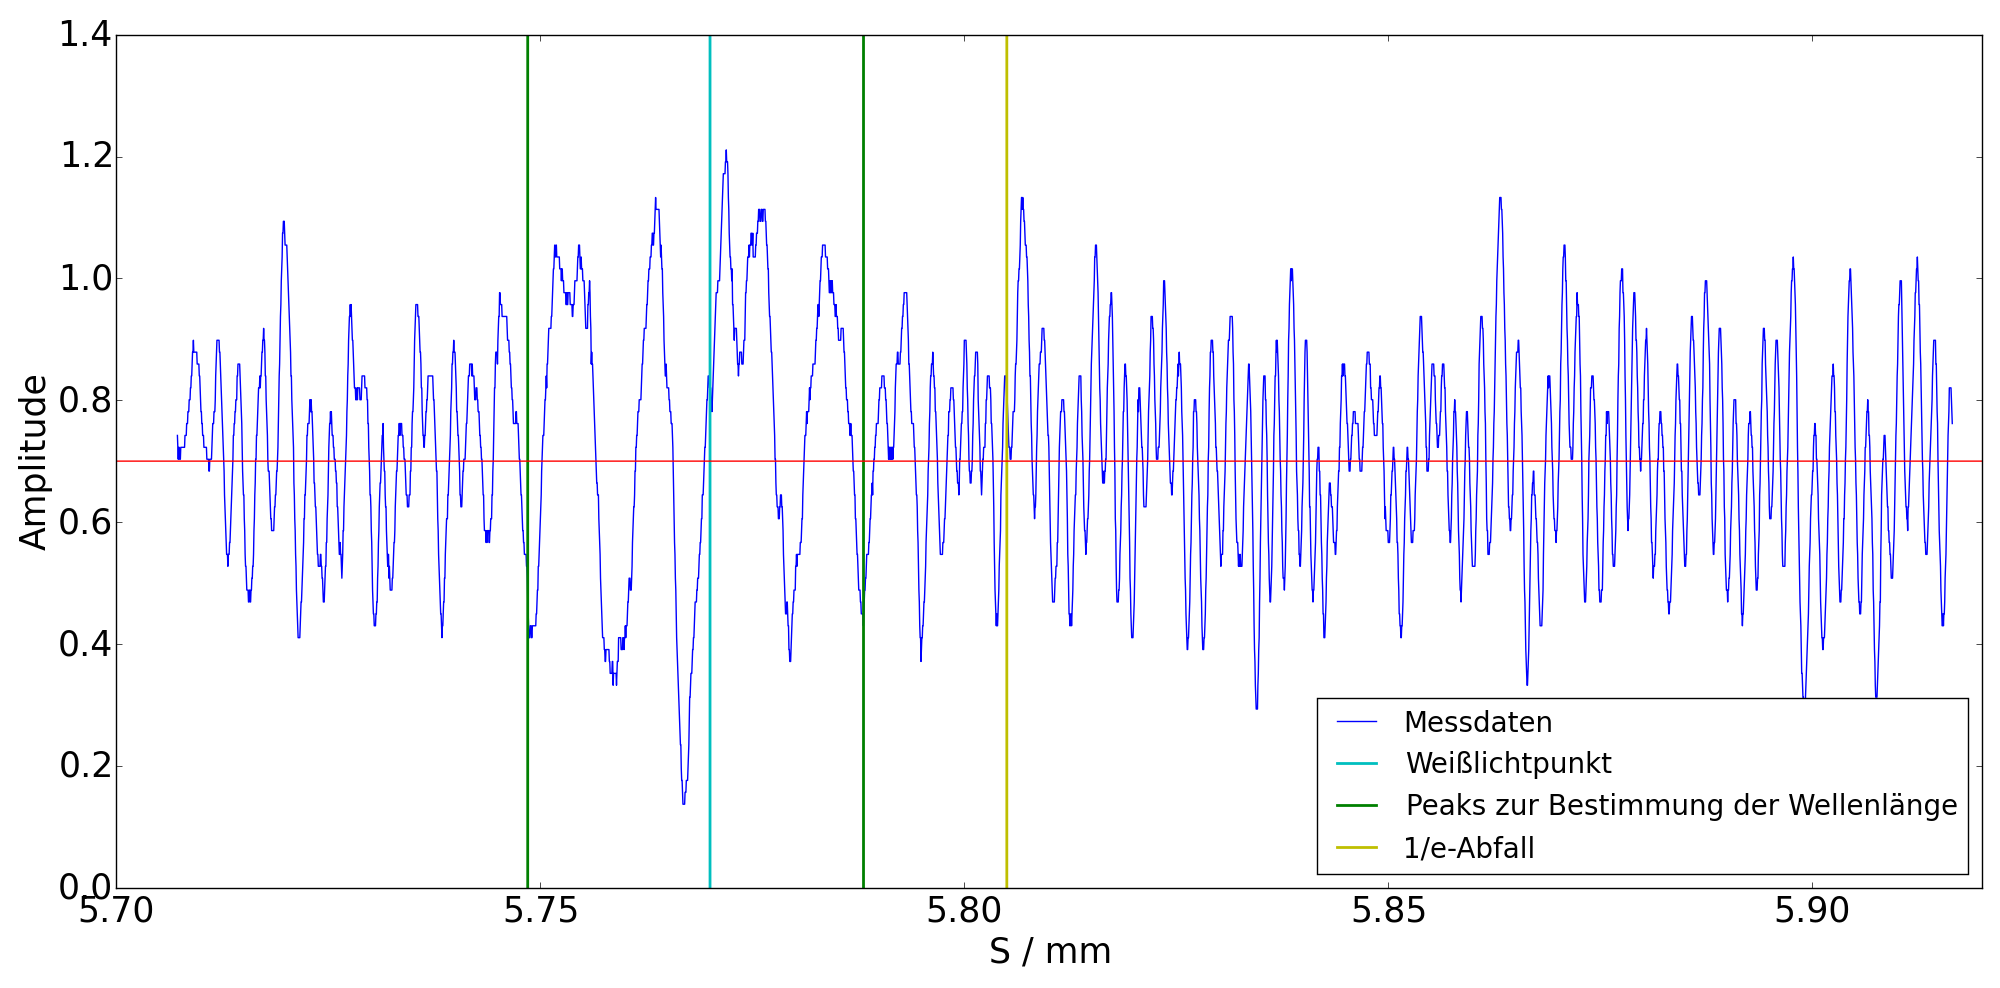
\includegraphics[scale = 0.32]{filter_weiss.png}
\caption{Interferogramm f�r den Muffelofen mit Schmalbandfilter. Die gr�nen Linien markieren den Bereich f�r die Bestimmung der Wellenl�nge, die rote Linie markiert die Nulllage}
\label{fig:filter_weiss}
\end{figure}

Aus den Interferrogramm ergeben sich die Werte in Tabelle \ref{tab:parameter_filter}. Es wurde ein kleines Intervall um den Wei�lichtpunkt gew�hlt, da in diesem Bereich die Abst�nde zwischen den Peaks regelm��ig sind. Aus den Werten ergibt sich eine Wellenl�nge von 2.91(5)$\mu$m, dieser Wert weicht um 39,82\% vom Literaturwert von 3,31$\mu$m ab (Quelle:\cite{Staatsex_Michels}). Mit diesem Wert l�sst sich der Parameter b aus Gleichung \ref{eqn:B_schmalband} bestimmten.

\begin{align}
b = \frac{2 \pi}{\lambda} = 1.988(3) \frac{1}{\mu m}
\end{align}

\begin{table}[H]
\centering
\caption{Messwerte f�r die Bestimmung der Wellenl�nge des Wei�lichtpunkts}
\label{tab:parameter_filter}
\begin{tabular}{|c|c|c|c|}
\hline x$_1$ / mm & x$_2$ / mm & s / mm & n \\ 
\hline 5,7485(3) & 5,7881(3) & 0,0396(4) & 5 \\ 
\hline 
\end{tabular} 
\end{table}

F�r die Bestimmung des 1/e-Abfalls wird die Position des Wei�lichtpunkts verwendet. Die Amplitude am Wei�lichtpunkt betr�gt ca. 0,57 V. Das Minimum des Interferogramms liegt bei ca. 0,4. Der 1/e-Abfall ergibt sich bei einer Position von 5.805(3) $\mu$m mit einer Amplitude von 0,208 V erreicht. Dadurch ergibt sich eine Breite des 1/e-Abfalls von 0,35(2) mm. Aus den Werten l�sst sich die spektrale Verteilung des Ofens bestimmen. Die Wellenzahlen ergeben sich mit: 

\begin{align}
\bar{\nu_1} = b - \frac{2}{a} = 1,93(4) \mu m^{-1}\\
\bar{\nu_2} = b - \frac{2}{a} = 2,04(4) \mu m^{-1}
\end{align}

Aus den beiden Werten l�sst sich nach \cite{Staatsex_Michels} die e$^{-1}$-Breite $\Delta \lambda$ des Schmalbandfilters bestimmen.

\begin{align}
\Delta \lambda = \frac{1}{\bar{\nu_1}} - \frac{1}{\bar{\nu_2}}= 0,289(8) \mu m
\end{align}

Erwartet wurde ein Wert von 0,060 $\mu$m \cite{Staatsex_Michels}. Der Bestimmte Wert liegt ca. eine Gr��enordnung �ber halb des theoretischen Wertes, dies kommt wahrscheinlich von dem ungenau bestimmten a. 

Aus den beiden Parametern a und b ergibt sich die spektrale Verteilung des Muffelofen in Abbildung \ref{fig:spektrum_filter}.

\begin{figure}[H]
\centering
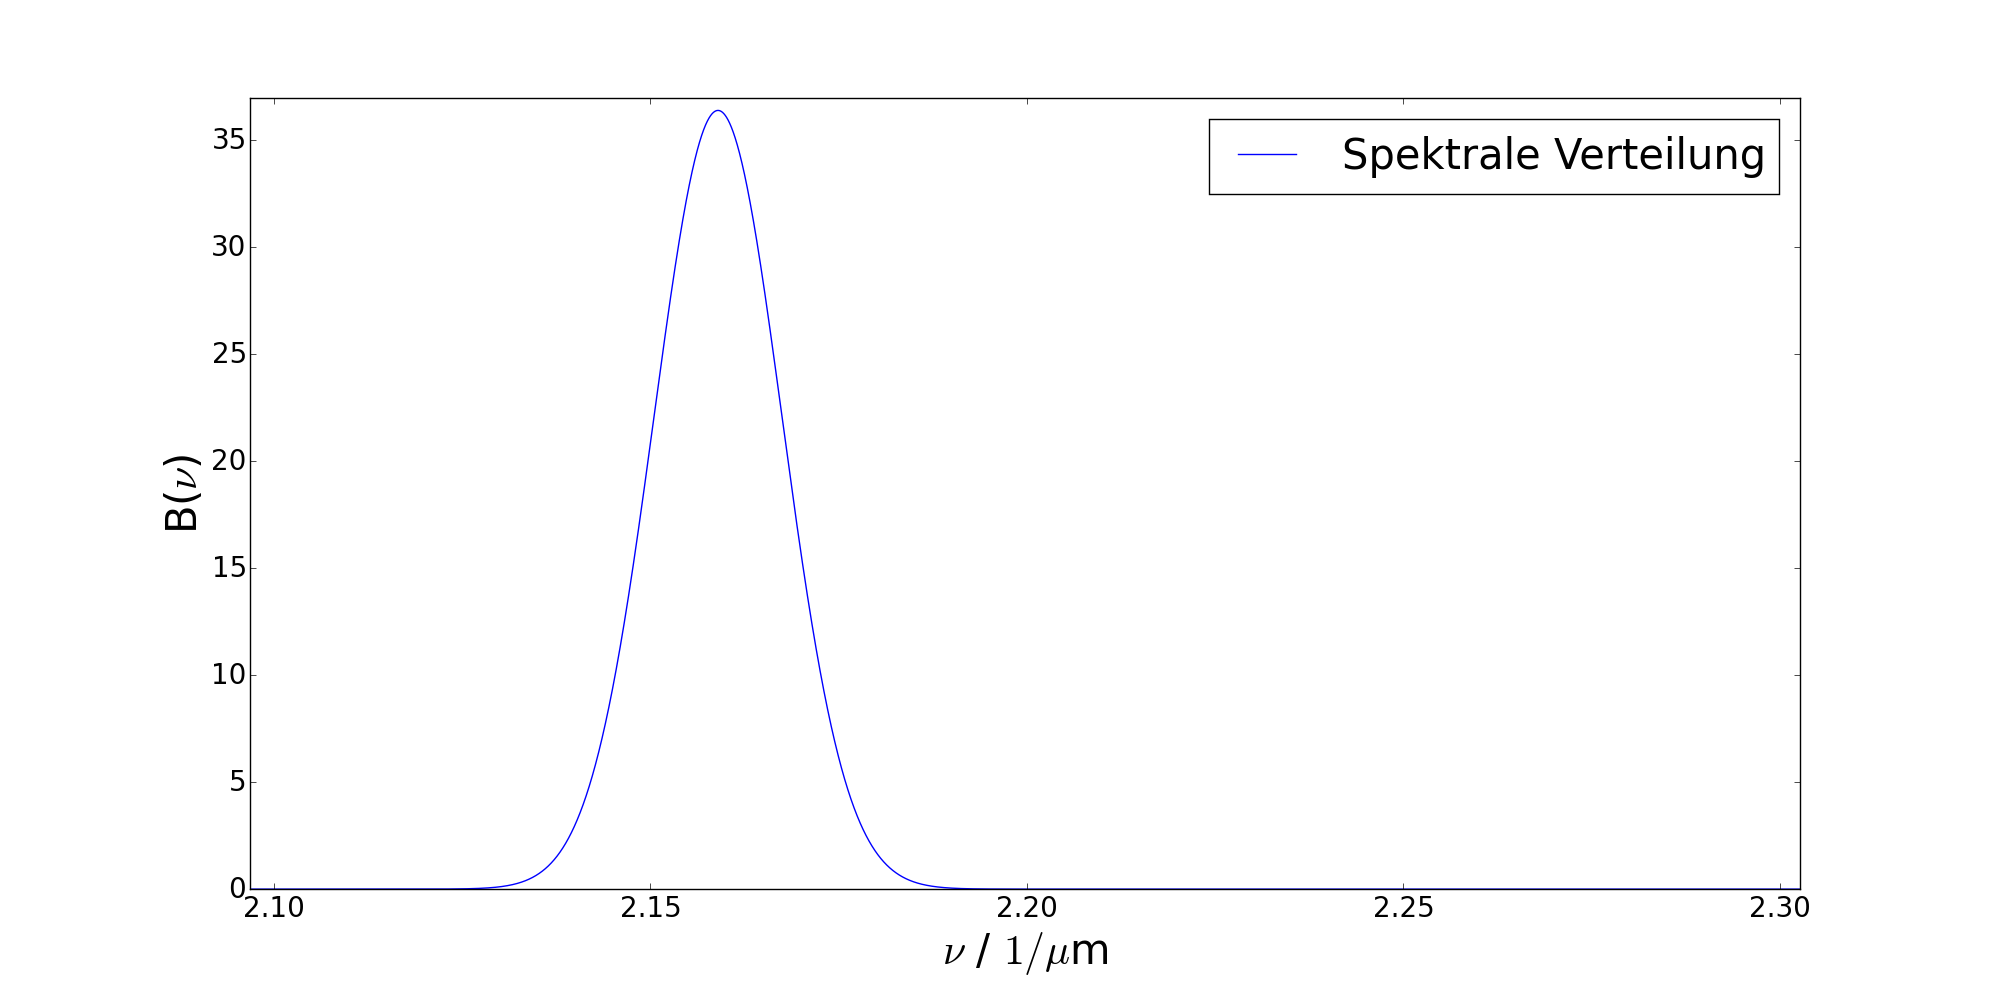
\includegraphics[scale = 0.33]{verteilung_filter.png}
\caption{Spektrale Verteilung des Schmalbandfilters}
\label{fig:spektrum_filter}
\end{figure}

Zum Schluss soll erw�hnt werden, dass bei Anwendung einer FFT, eines Algorithmusses f�r die diskrete Fouriertransformation, ein �hnliches Ergebnis zustande kommt. Da die FFT f�r periodische Signale geeignet ist, kann zur Rauschunterdr�ckung eine sogenannte Fensterfunktion verwendet werden, welche das Signal 'sanft' ein und ausblendet. Das FFT-Spektrum ohne Fensterfunktion ist in Abbildung \ref{fig:fftfilterinterferogramm_ohne_fenster} dargestellt.
\begin{figure}[H]
\centering
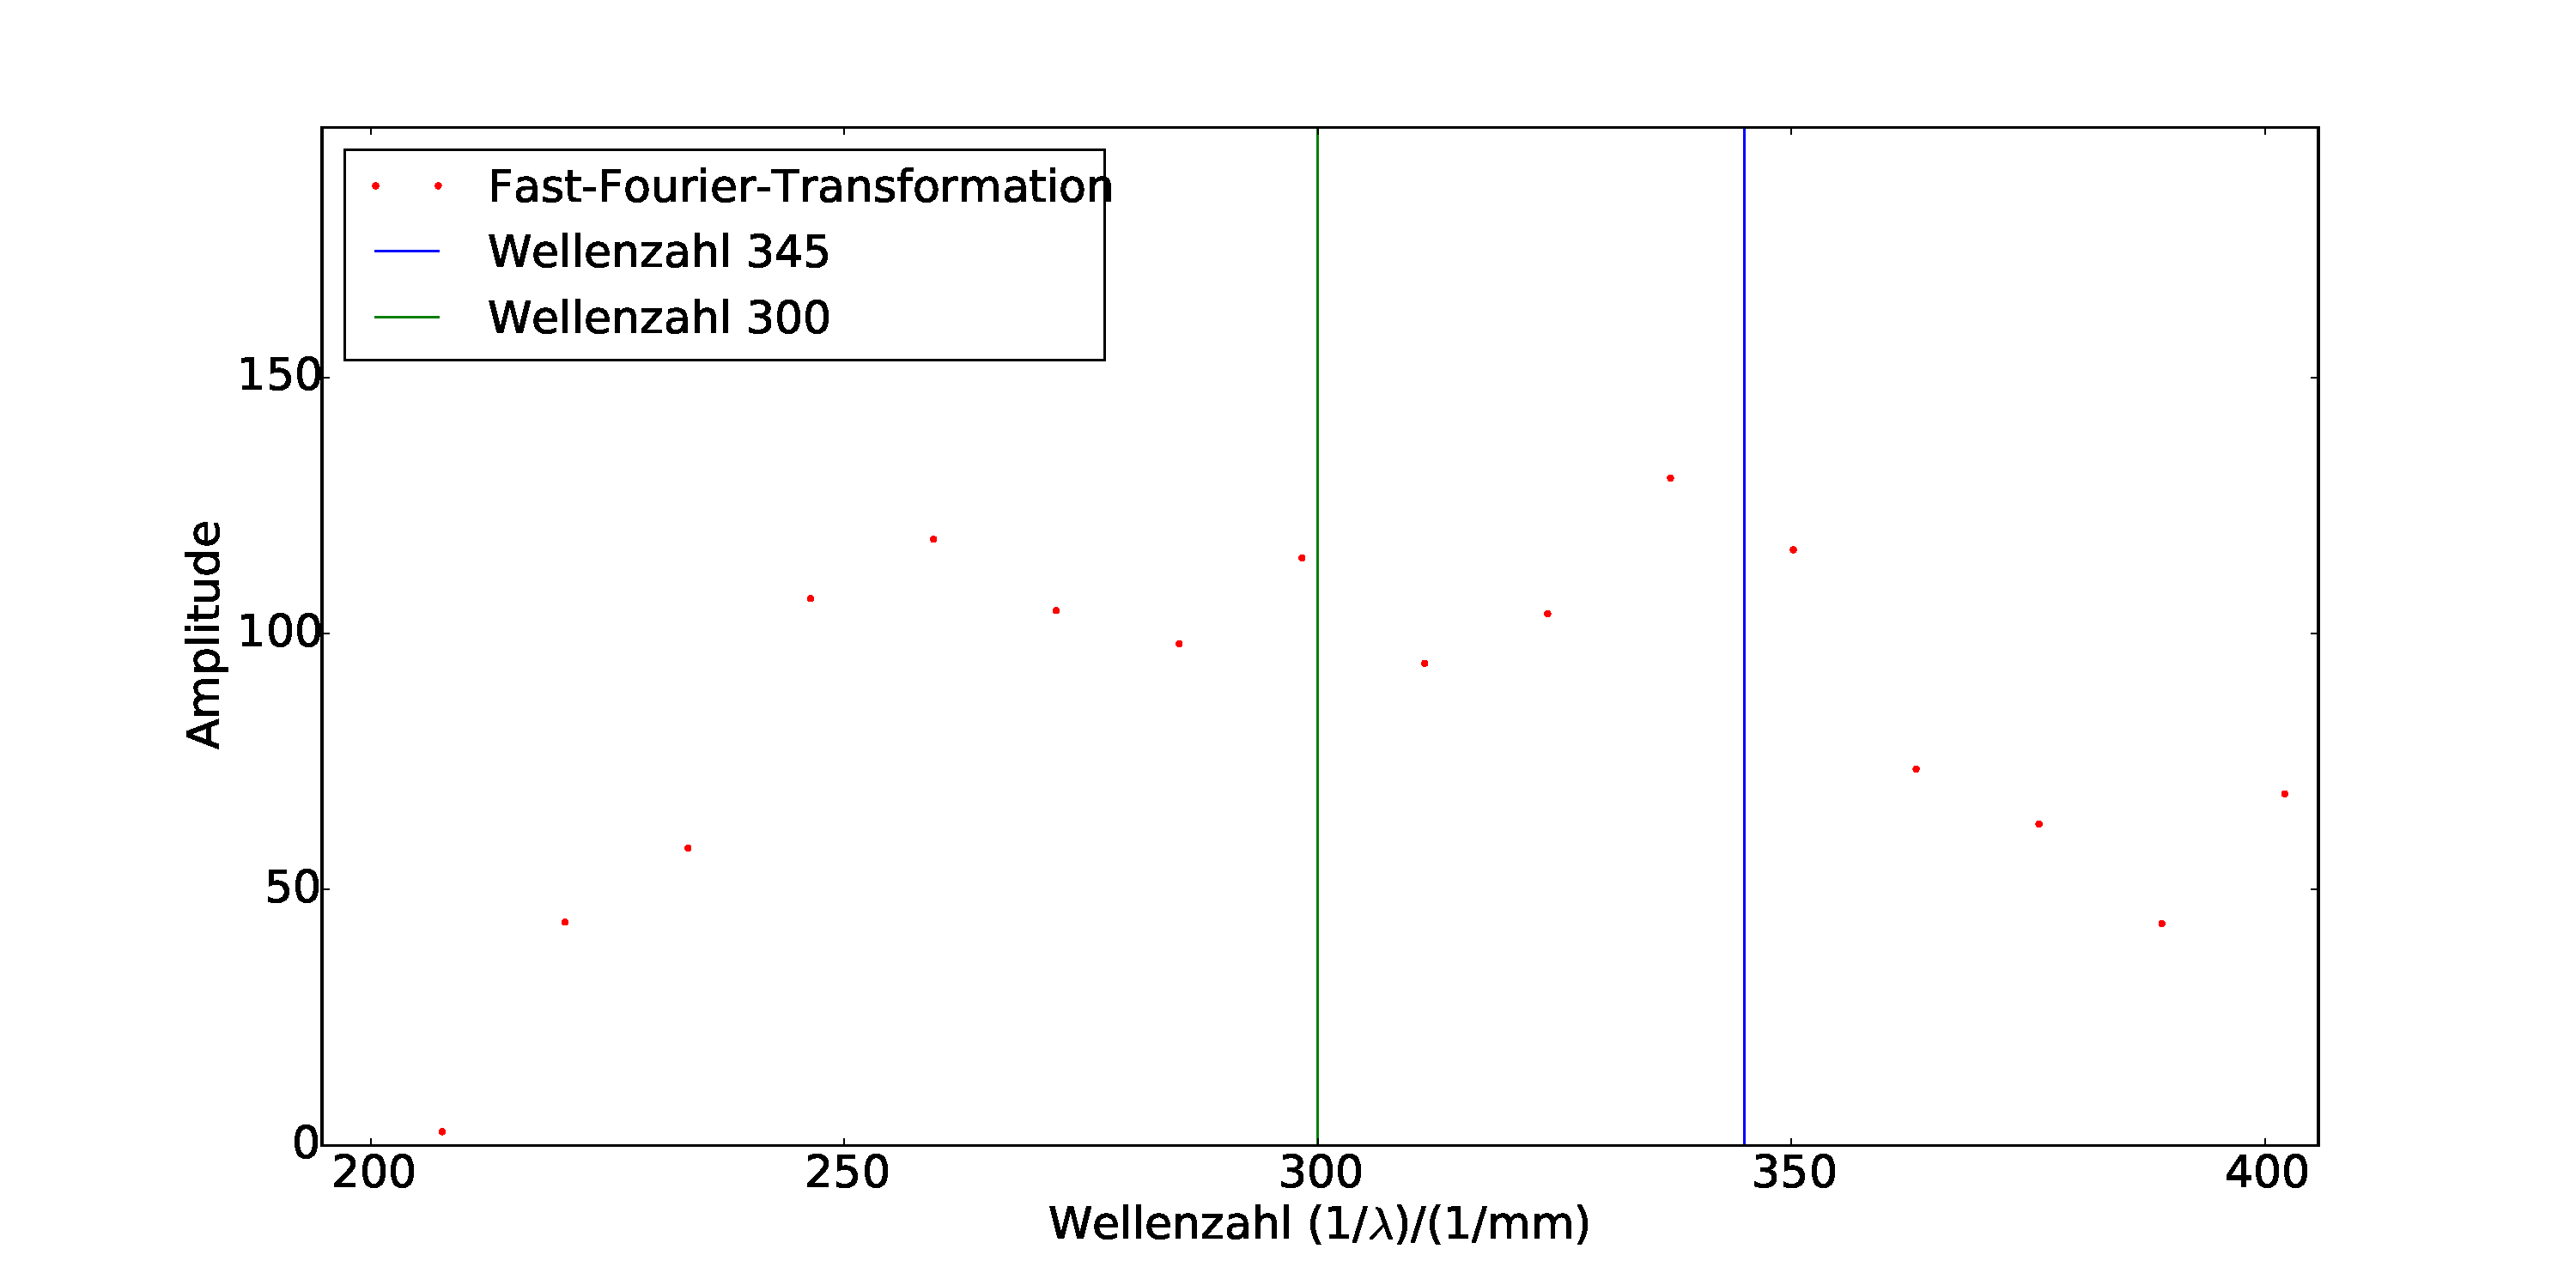
\includegraphics[scale = 0.38, clip = true, trim = 3cm 0cm 3cm 0cm]{Wellenzahlen200-400FilterohneFenster}
\caption{Diskrete Fouriertransformation des Filterinterferogramms f�r Wellenzahlen ($1/\lambda$) von \SI{200}{$\frac{1}{mm}$} bis \SI{400}{$\frac{1}{mm}$}  ohne Fensterfunktion (verrauscht)}
\label{fig:fftfilterinterferogramm_ohne_fenster}
\end{figure}
Man sieht, dass die Wellenzahl \SI{300(2)}{$\frac{1}{mm}$} im Spektrum vertreten ist, welche einer Wellenl�nge von \SI{3,33(2)}{$\mu$m} entspricht. Beim ein und Ausblenden des Signals mit den Funktionen $f(x)=(\frac{1-\cos(\frac{2 \pi x}{L})}{2})$ und $f(x)=(\frac{1-\cos(\frac{2 \pi x}{L})}{2})^4$, um das Rauschen durch die Nichtperiodizit�t zu unterdr�cken, wird diese Wellenzahl jedoch herausgefiltert. Die beiden Spektren, welche durch Anwendung der beiden Filterfunktionen entstehen, sind in den Abbildungen \ref{fig:fftfilterinterferogramm_k_1} und \ref{fig:fftfilterinterferogramm_k_4} dargestellt.
\begin{figure}[H]
\begin{subfigure}[t]{0.49\textwidth}
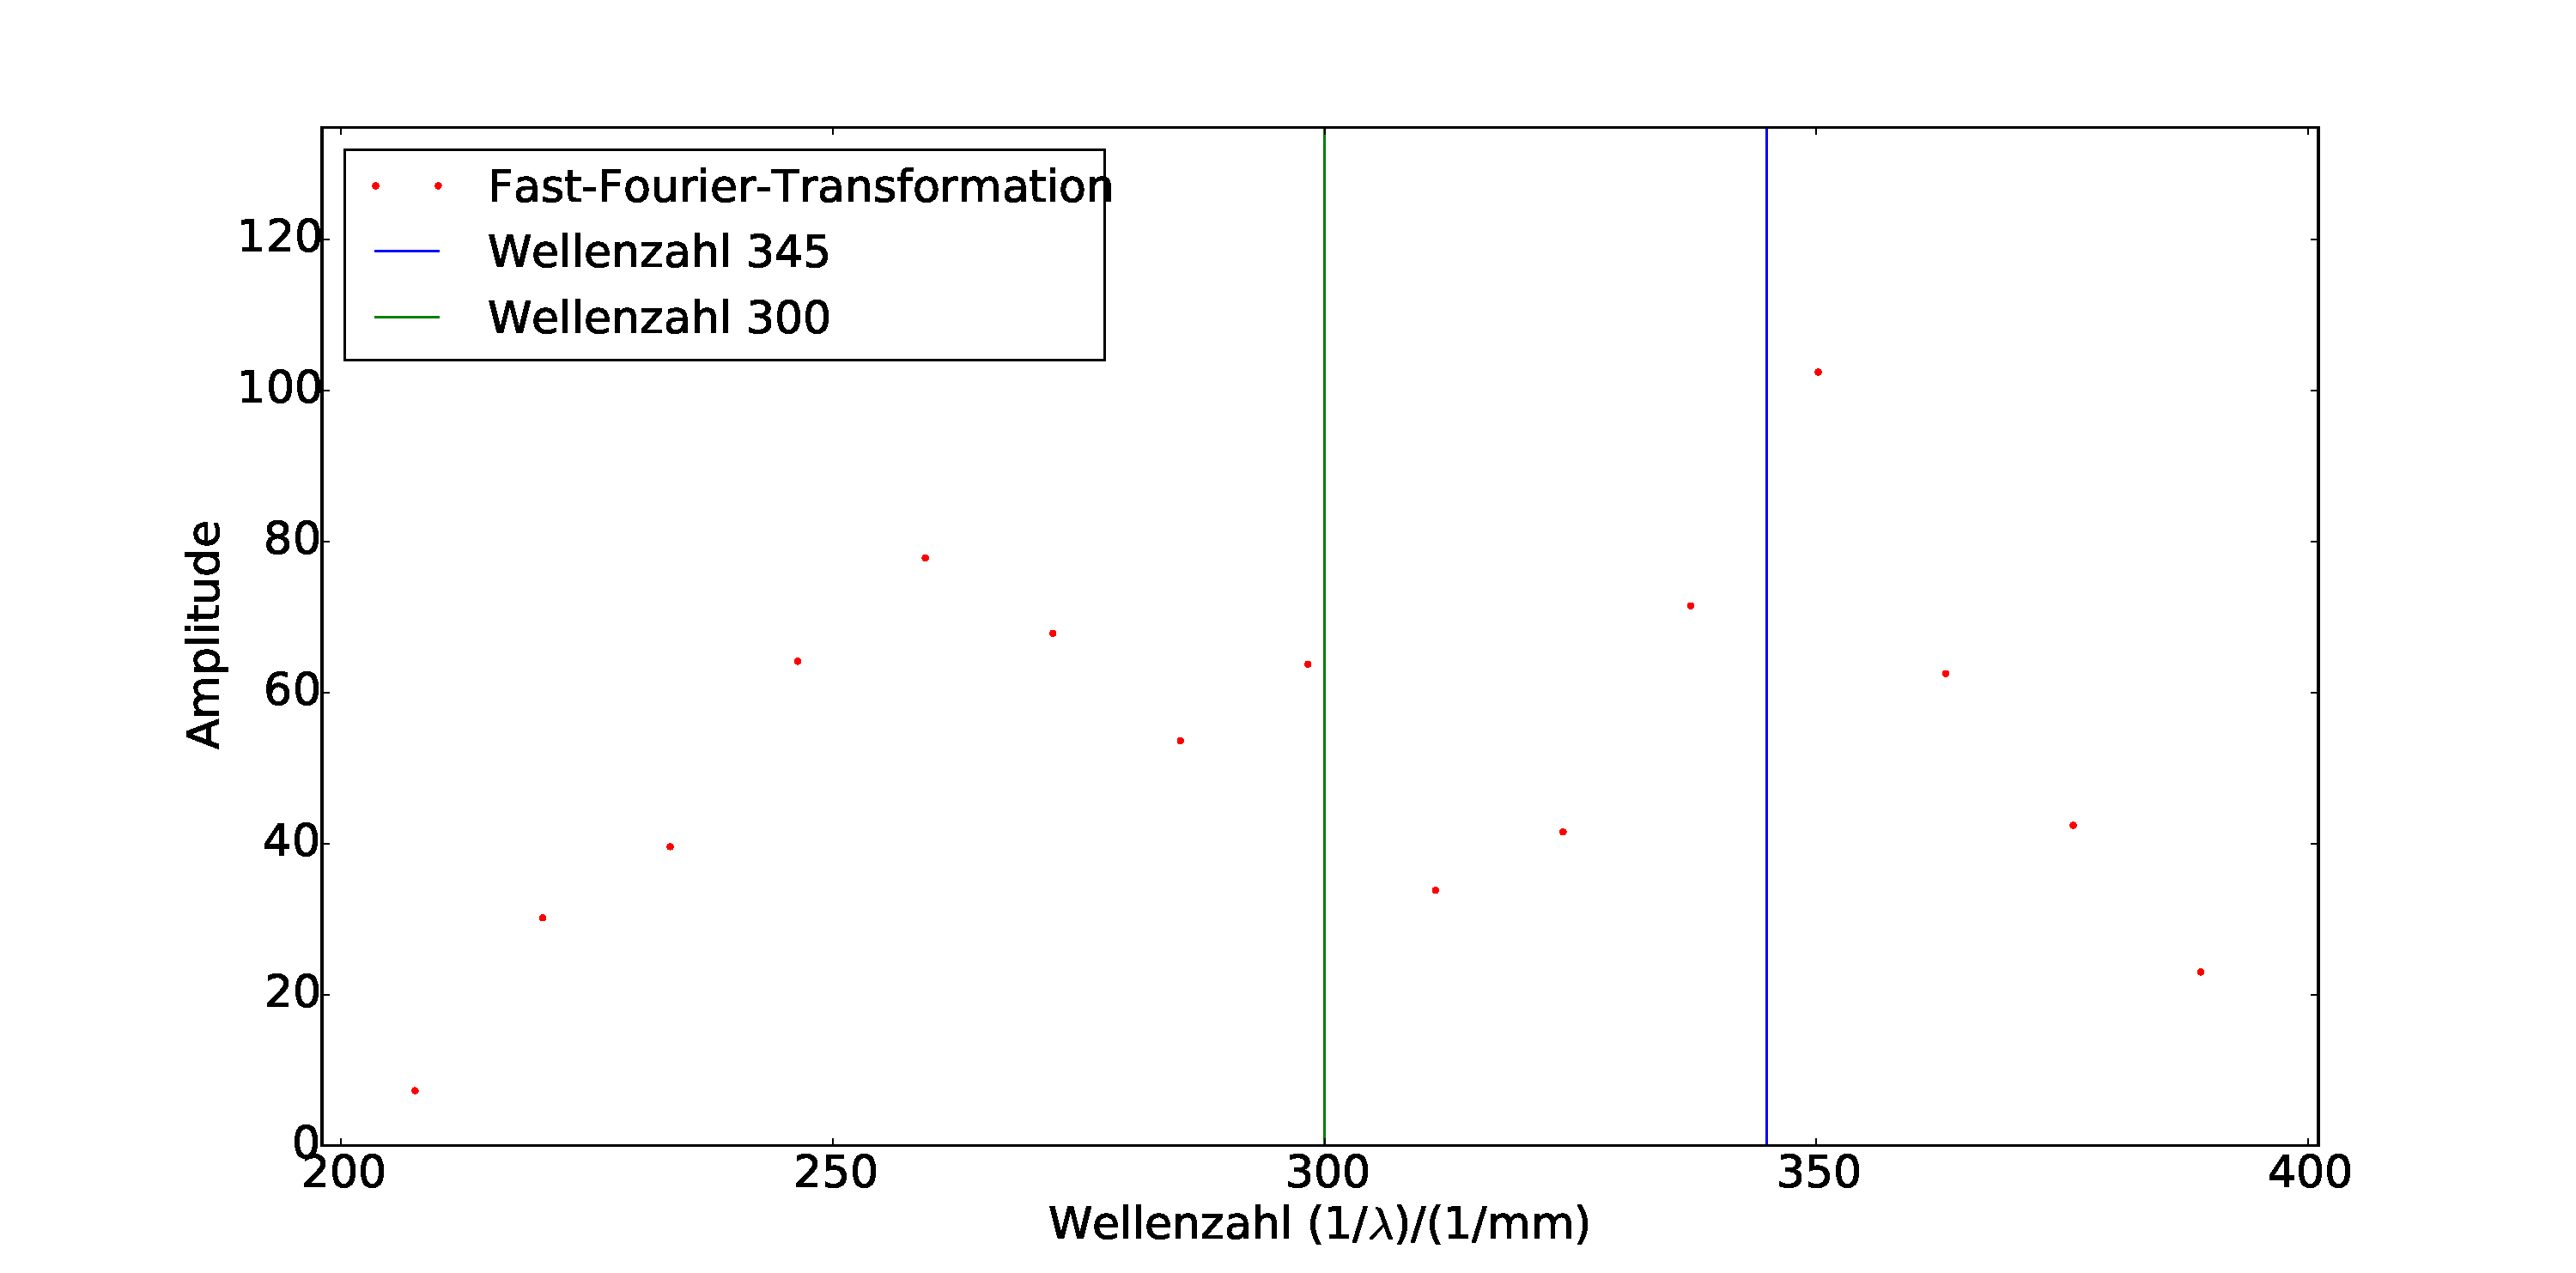
\includegraphics[scale = 0.19, clip = true, trim = 3cm 0cm 3cm 0cm]{Wellenzahlen200-400FiltermitFenster(0,5*(1-cos))}
\caption{Diskrete Fouriertransformation des Filterinterferogramms f�r Wellenzahlen ($1/\lambda$) von \SI{200}{$\frac{1}{mm}$} bis \SI{400}{$\frac{1}{mm}$} mit Fensterfunktion\\$f(x)=(\frac{1-\cos(\frac{2 \pi x}{L})}{2})$}
\label{fig:fftfilterinterferogramm_k_1}
\end{subfigure}
\hspace{0.02\textwidth}
\begin{subfigure}[t]{0.49\textwidth}
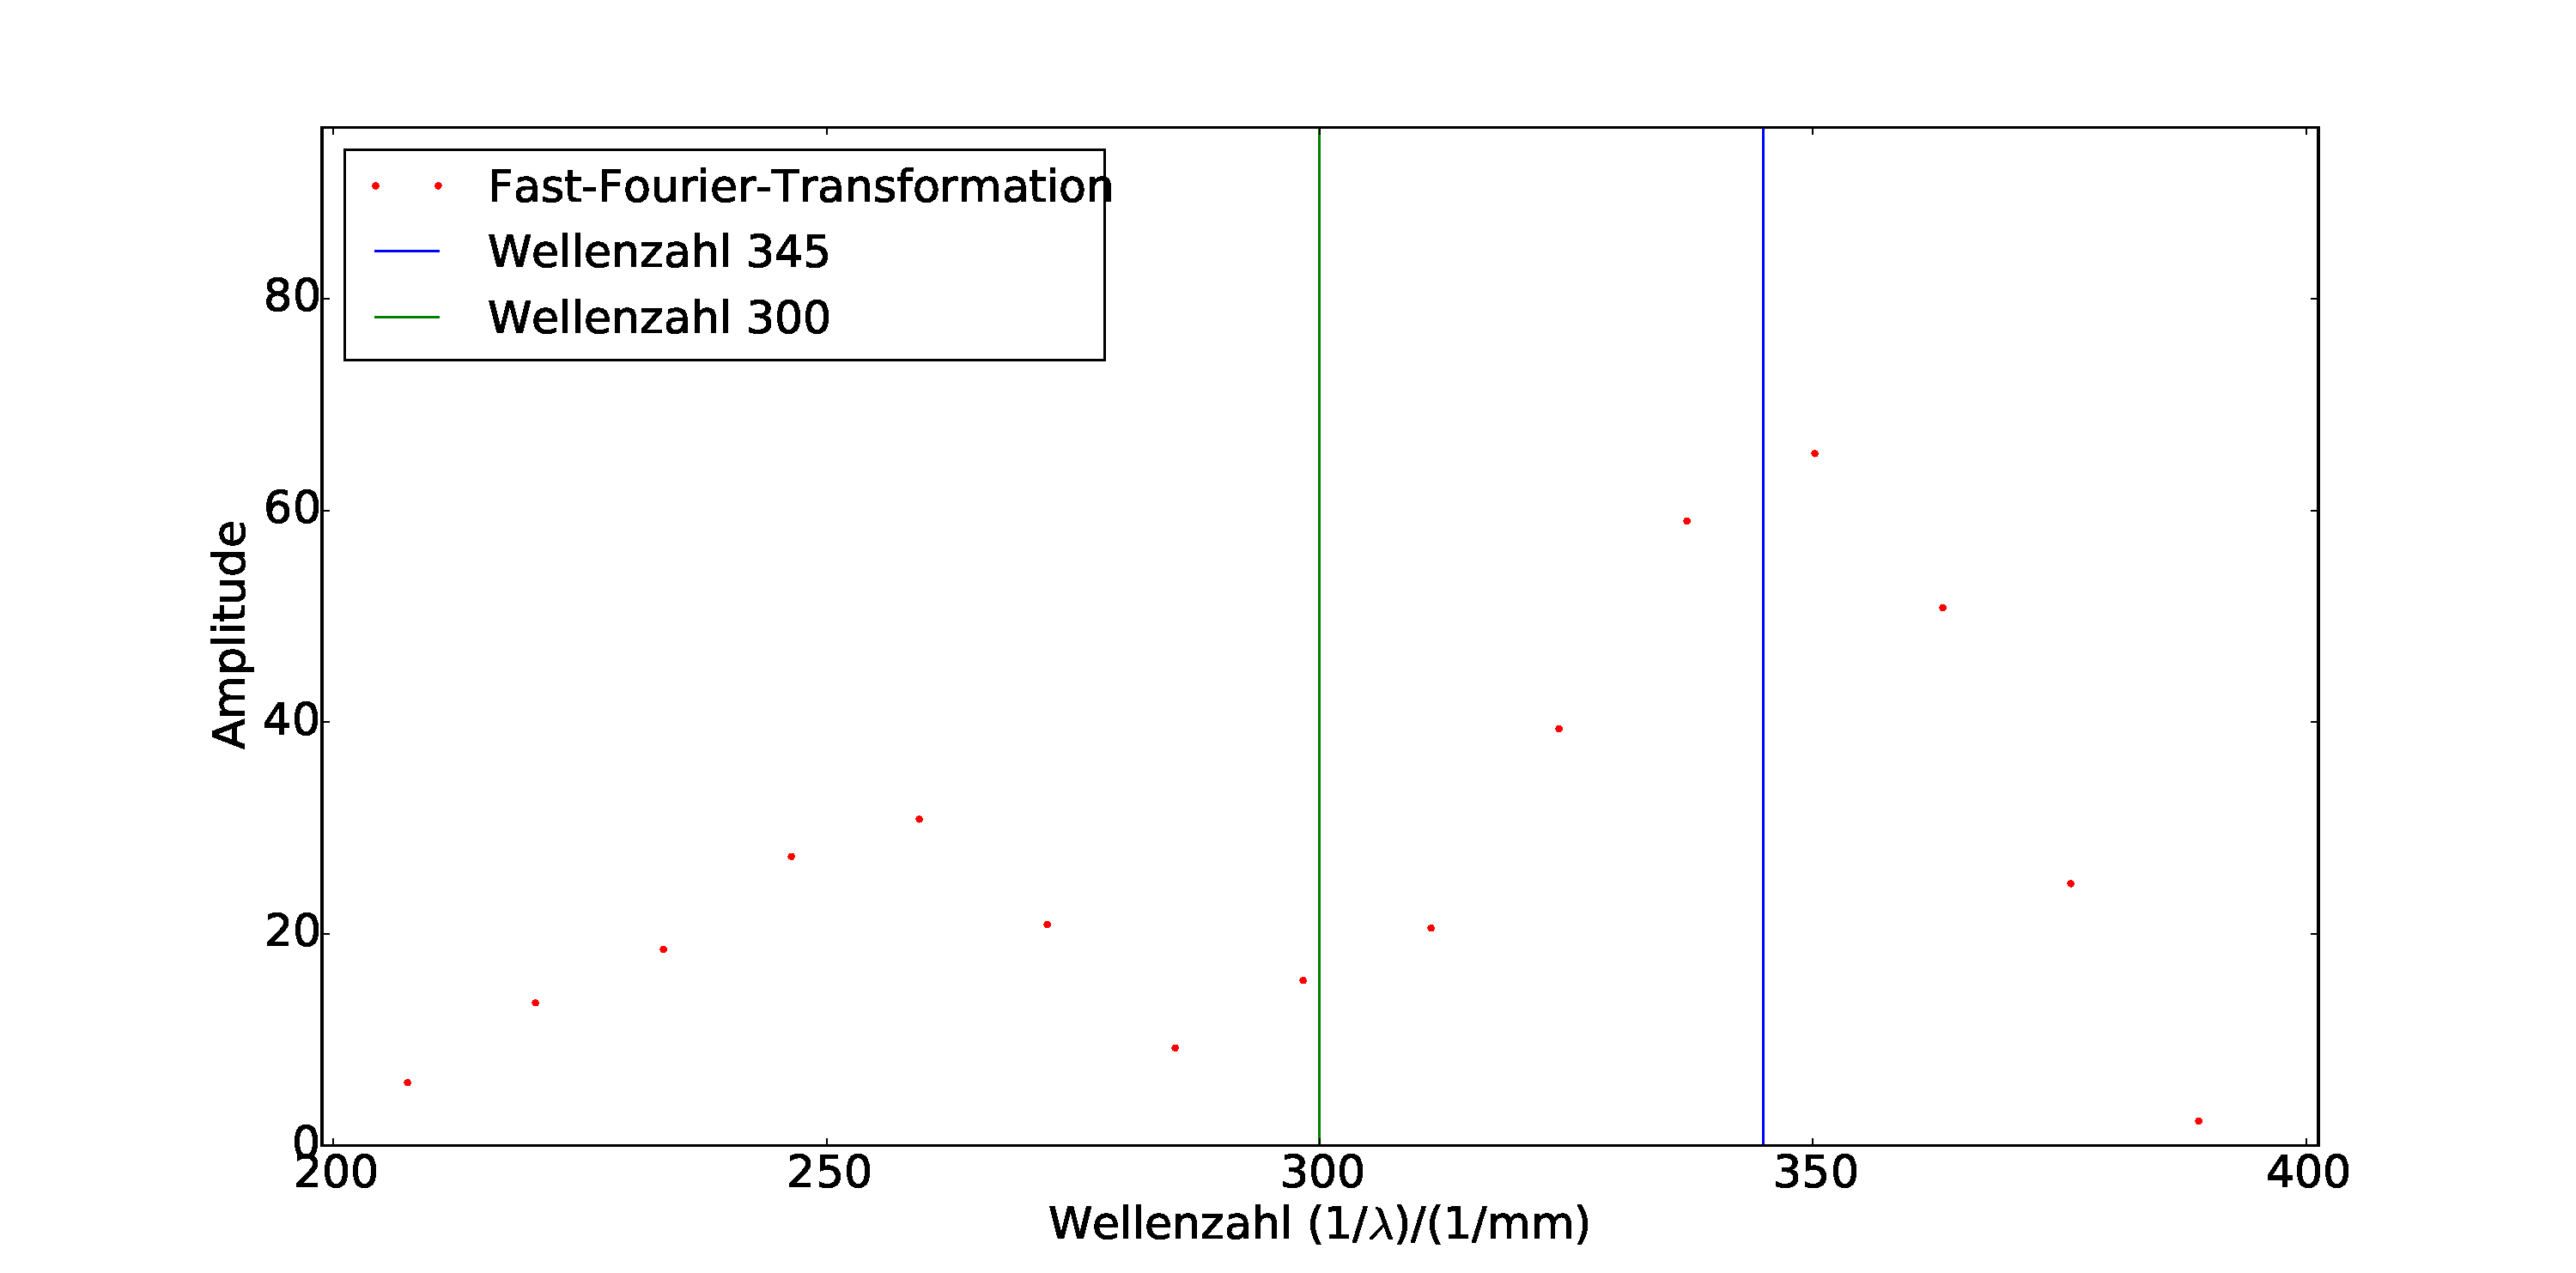
\includegraphics[scale = 0.19, clip = true, trim = 3cm 0cm 3cm 0cm]{Wellenzahlen200-400FiltermitFenster(0,5*(1-cos))**4}
\caption{Diskrete Fouriertransformation des Filterinterferogramms f�r Wellenzahlen ($1/\lambda$) von \SI{200}{$\frac{1}{mm}$} bis \SI{400}{$\frac{1}{mm}$} mit Fensterfunktion\\$f(x)=(\frac{1-\cos(\frac{2 \pi x}{L})}{2})^4$}
\label{fig:fftfilterinterferogramm_k_4}
\end{subfigure}
\end{figure}
Man sieht, dass der gr��te Peak, mit der Fensterfunktion $f(x)=(\frac{1-\cos(\frac{2 \pi x}{L})}{2})^k$ ($k=1,4$) bei einer Wellenzahl von \SI{345(2)}{$\frac{1}{mm}$} liegt, was einer Wellenl�nge von \SI{2,90(2)}{$\mu$m} entspricht. Diese stimmt mit der manuell bestimmten Wellenl�nge von \SI{2,91(5)}{$\mu$m} zu \SI{99,7}{\percent} �berein. Dieses Ergebnis spricht f�r die Konsistenz der manuellen Messung.
\subsection{Analyse des Schwebungsinterferogramms}
In diesem Versuchsteil soll die Schwebung zweier nahe beieinander liegender Signale untersucht werden. Die verwendeten Wellenl�ngen liegen bei \SI{3.31}{$\mu$m} (Muffelofen mit Filter) und \SI{3.39}{$\mu$m} (He-Ne-Laser). Um die Schwebung sichbar zu machen, musste die Amplitude des He-Ne-Lasers an die Amplitude des gefilterten Muffelofenspektrums angepasst werden. Dazu wurden Polyethylenfolien in den Strahlengang des Lasers montiert, welche zur Feinjustierung verkippt werden konnten. Die Eichung wurde f�r diese Messung wie in Abschnitt \ref{Eichung} durchgef�hrt. Der Plot f�r die Eichung und die Fitfunktion ist im Anhang Abschnitt \ref{Schwebung} zu finden. Das Interferogramm zur Analyse der Schwebung ist in Abbildung \ref{fig:schwebungsinterferogramm} zu sehen.
\begin{figure}[H]
\centering
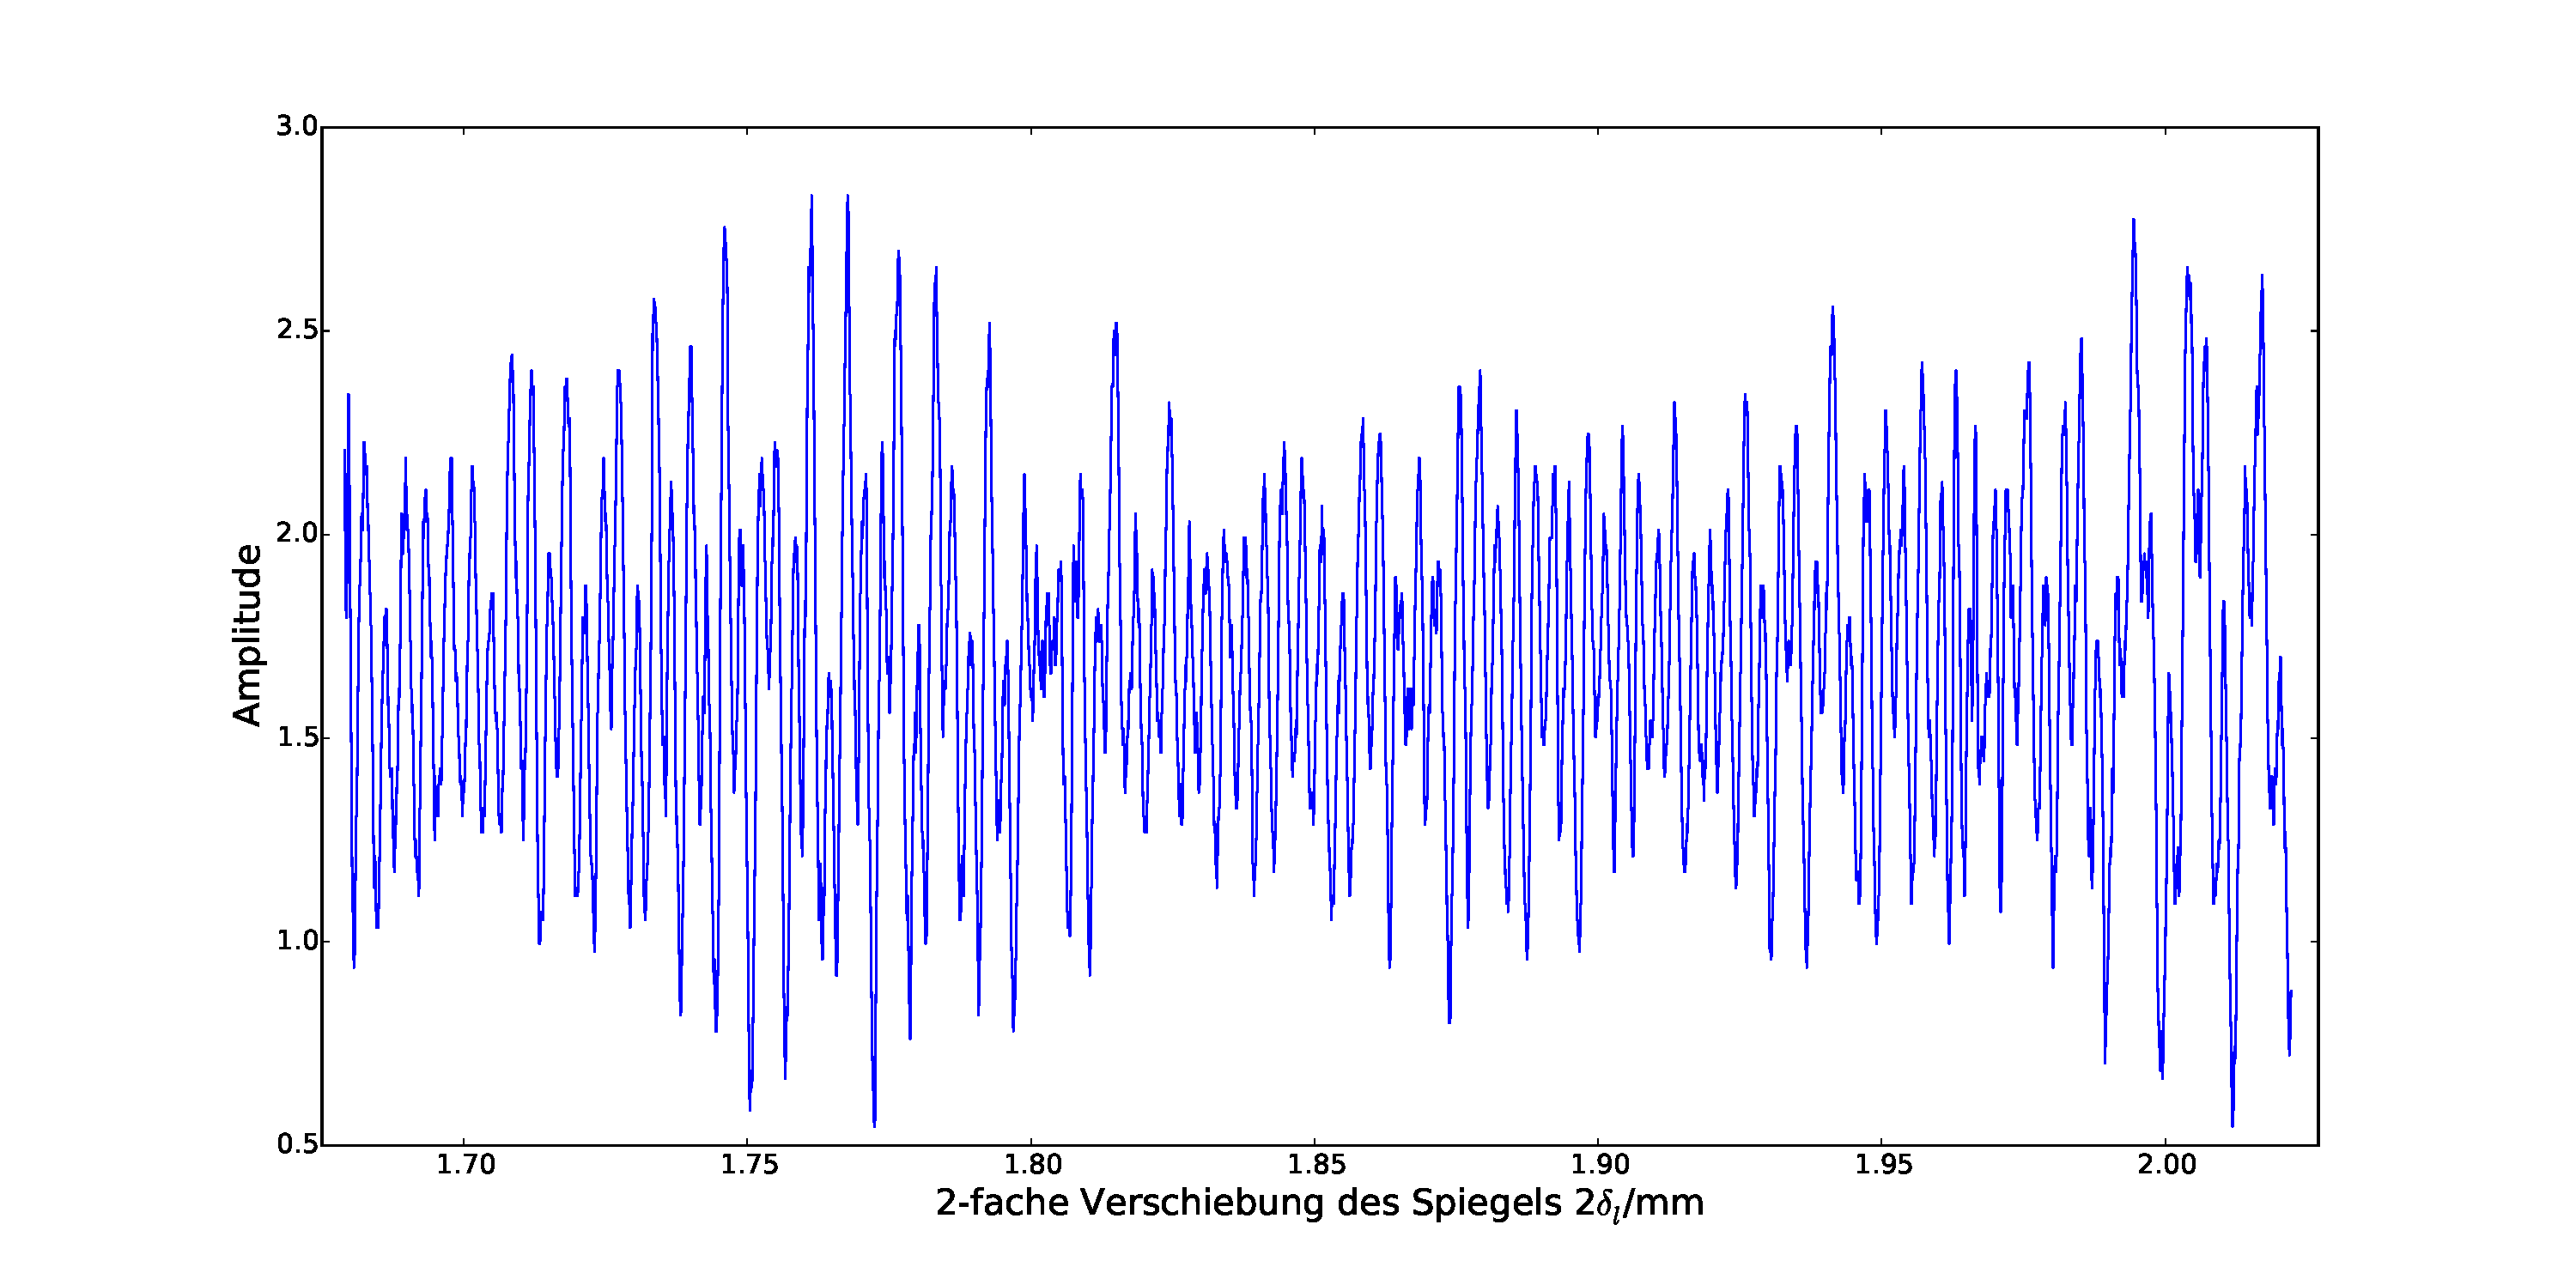
\includegraphics[scale = 0.38, clip = true, trim = 3cm 0cm 3cm 0cm]{Schwebung_Daten}
\caption{Schwebungsinterferogramm}
\label{fig:schwebungsinterferogramm}
\end{figure}
Da die Wellenl�nge der in dem Interferogramm erkennbaren Schwebung sehr stark von der erwarteten Schwebungswellenl�nge abweicht, wird es hier vorgezogen, einen FFT-Algorithmus (Fast-Fourier-Transform) f�r die diskrete Fouriertransformation zu verwenden, um herauszufinden, welche Wellenzahlen (1/$\lambda$) in dem Interferogramm vertreten sind. Auf eine Herleitung der DFT und deren Anwendung in der Analyse von Daten wird verzichtet, da dies lediglich einer Diskretisierung der Fouriertransformation entspricht, wodurch 'gesamplete' Messdaten und deren Frequenzen analysiert werden k�nnen. Die diskrete Fouriertransformation ist f�r die Analyse periodischer Signale geeignet, sodass bei der Analyse nichtperiodischer Signale hochfrequente Anteile in der Fouriertransformation hinzukommen, welche in den niedrigfrequenten Bereich gespiegelt werden, da $f(t)=e^{2\pi i nt/N}$ keine reelle Funktion ist. Dadurch sind die Daten nach der FFT stark verrauscht. Diese sind in Abbildung \ref{fig:fftschwebungsinterferogramm_ohne_fenster} dargestellt. Die FFT wurde auf das gesamte Interferogramm angewendet.
\begin{figure}[H]
\centering
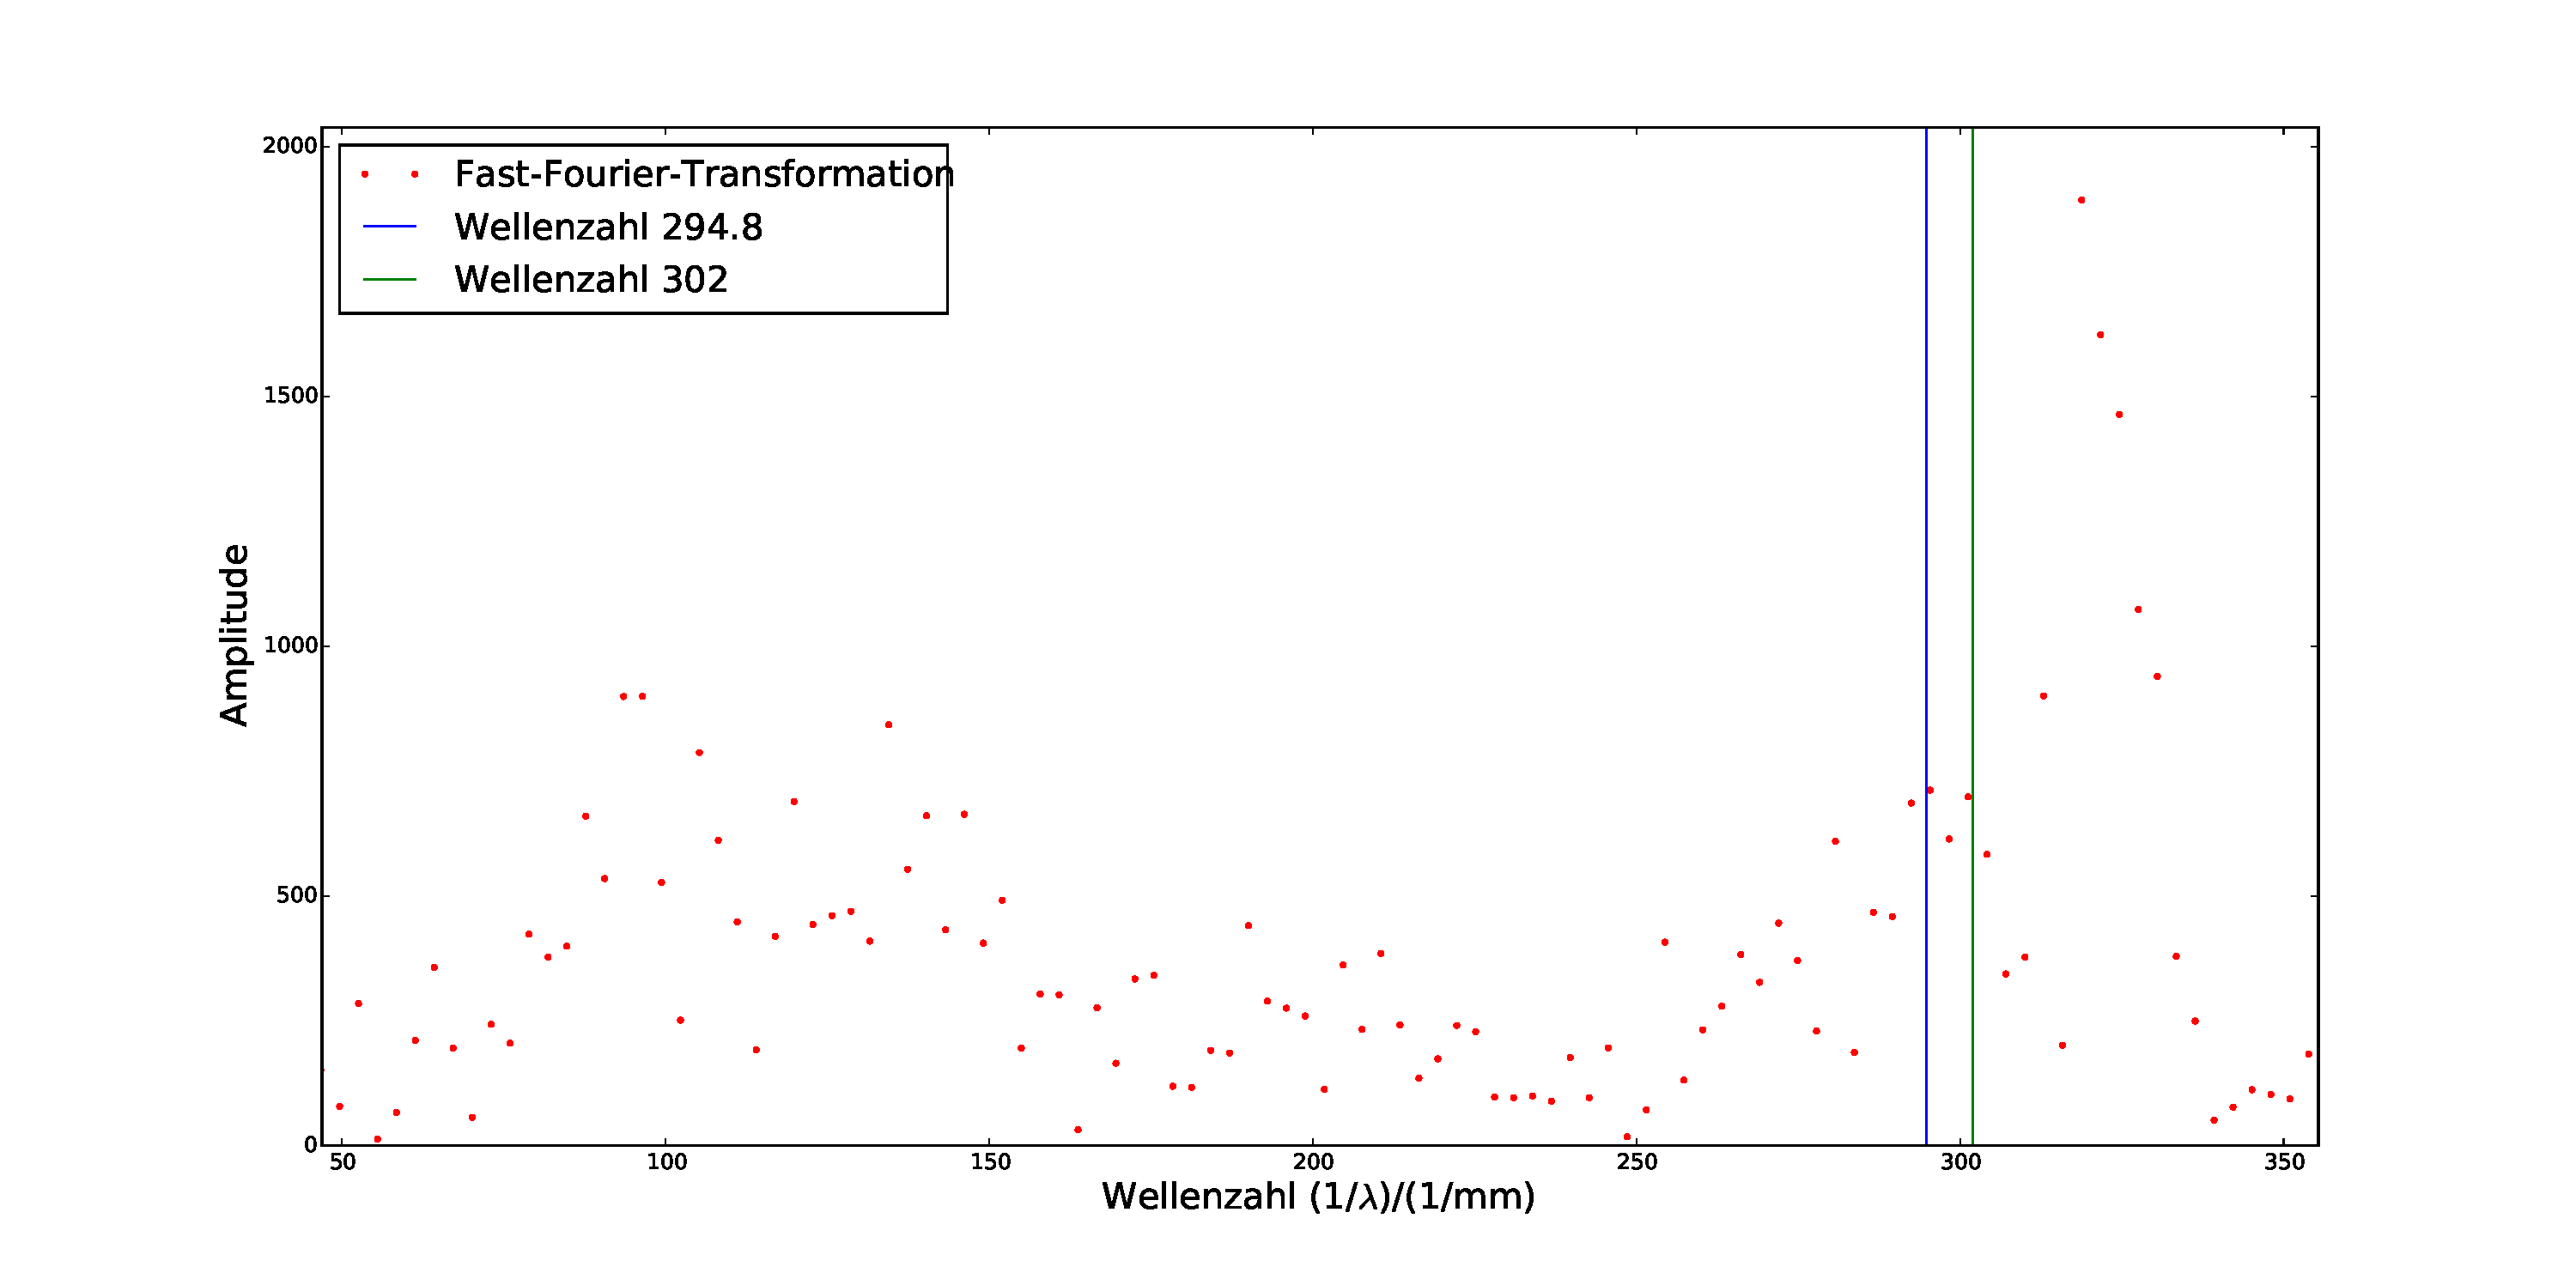
\includegraphics[scale = 0.38, clip = true, trim = 3cm 0cm 3cm 0cm]{Wellenzahlen50-350SchwebungohneFenster}
\caption{Diskrete Fouriertransformation des Schwebungsinterferogramms f�r Wellenzahlen ($1/\lambda$) von \SI{50}{$\frac{1}{mm}$} bis \SI{350}{$\frac{1}{mm}$}  ohne Fensterfunktion (verrauscht)}
\label{fig:fftschwebungsinterferogramm_ohne_fenster}
\end{figure}
Um die vertretenen Wellenzahlen aus dem Interferogramm abzulesen, wurde der Bereich \SI{260}{$\frac{1}{mm}$} bis \SI{315}{$\frac{1}{mm}$} n�her untersucht. Dieser ist in Abbildung \ref{fig:fftschwebungsinterferogramm} zu sehen.
\begin{figure}[H]
\centering
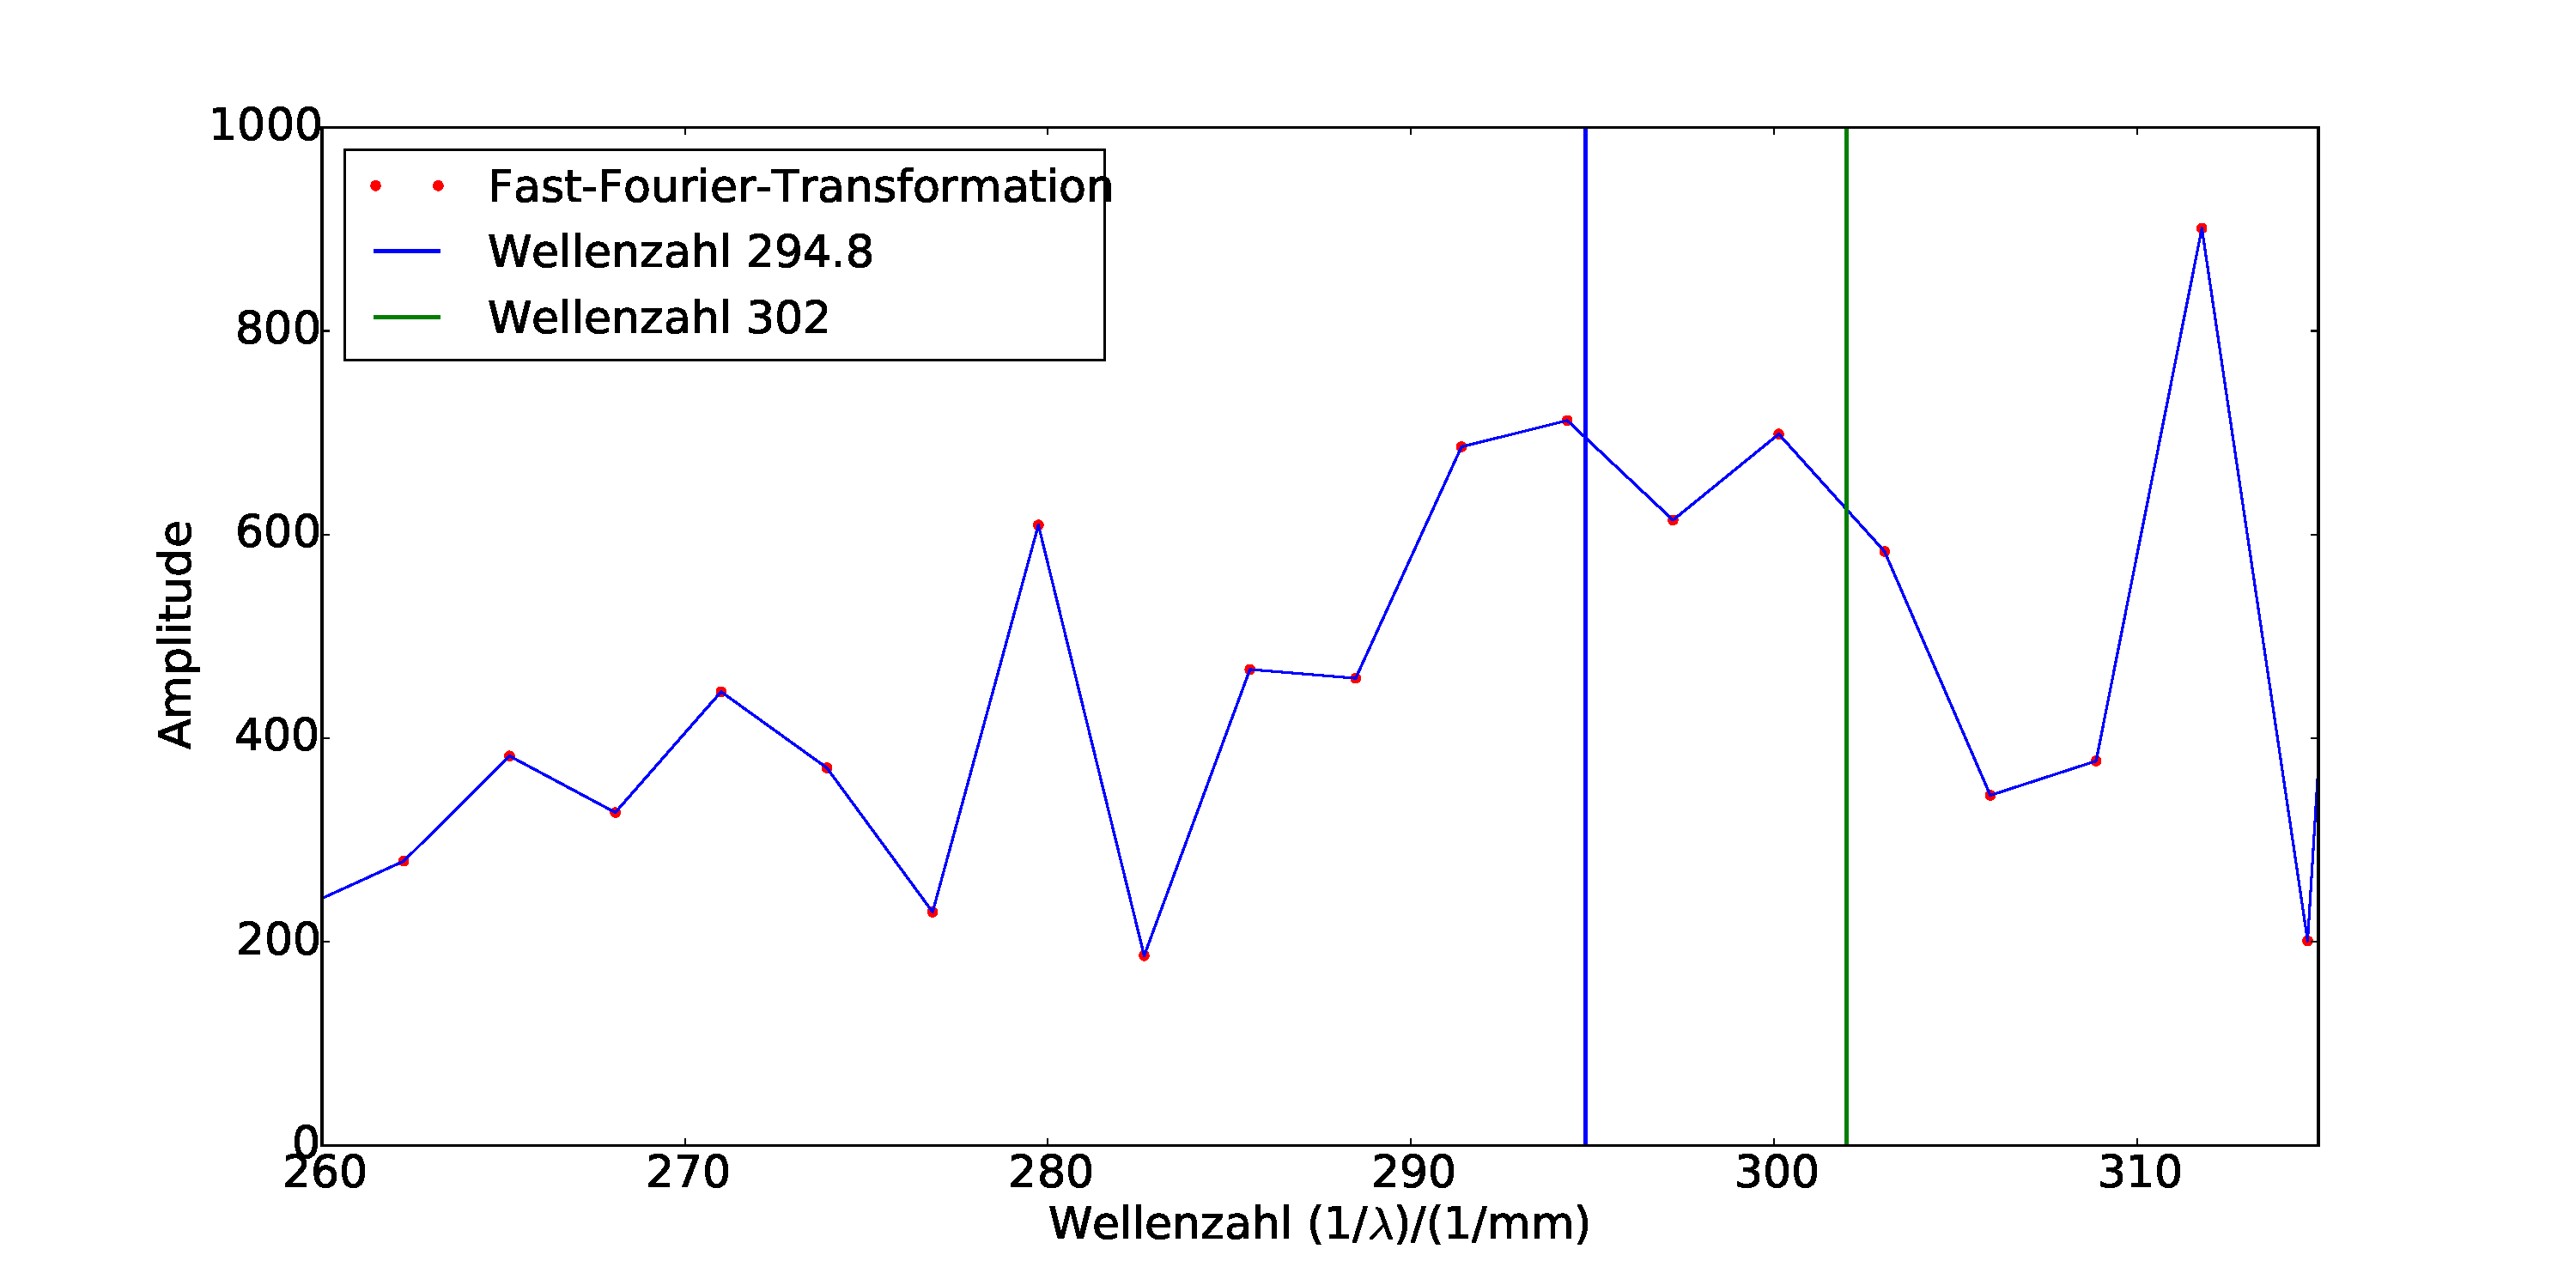
\includegraphics[scale = 0.38, clip = true, trim = 3cm 0cm 3cm 0cm]{Wellenzahlen260-340SchwebungohneFenster}
\caption{Diskrete Fouriertransformation des Schwebungsinterferogramms f�r Wellenzahlen ($1/\lambda$) von \SI{260}{$\frac{1}{mm}$} bis \SI{315}{$\frac{1}{mm}$}  ohne Fensterfunktion (verrauscht)}
\label{fig:fftschwebungsinterferogramm}
\end{figure}
Man sieht, dass die Wellenzahlen \SI{294,8(10)}{$\frac{1}{mm}$} und \SI{302(2)}{$\frac{1}{mm}$}, welche den Wellenl�ngen \SI{3,392(12)}{$\mu$m} und \SI{3,31(2)}{$\mu$m} entsprechen, in dem Interferogramm vertreten sind. Diese weichen von den erwarteten Wellenl�ngen \SI{3,31}{$\mu$m} und \SI{3,39}{$\mu$m} um \SI{0}{\percent} bzw. \SI{0,05}{\percent} ab. Daneben sind andere Frequenzen st�rker in dem Interferogramm vertreten.
Um herauszufinden, ob diese durch die Nichtperiodizit�t zustandekommen, multipliziert man sogenannte Fensterfunktionen mit dem Interferogramm, welche das Signal 'sanft' ein und ausblenden. In diesem Fall wurde die Funktion $f(x)=(\frac{1-\cos(\frac{2 \pi x}{L})}{2})^k$, wobei L die L�nge des Interferogramms ist und $k$ eine nat�rliche Zahl, als Fensterfunktion gew�hlt. Dadurch wird das Signal periodisch und das Rauschen durch Randeffekte kleiner. Abh�ngig von der Gr��e $k$, wirde der mittlere Teil des Interferogramms unterschiedlich stark gewichtet. Deshalb wurden f�r $k$ die Werte 1, 4 und 10 eingesetzt. Die Spektren f�r den Wellenzahlbereich von \SI{50}{$\frac{1}{mm}$} bis \SI{350}{$\frac{1}{mm}$} sind in Abbildung \ref{fig:fftschwebungsinterferogramm_k_1} ($k=1$), \ref{fig:fftschwebungsinterferogramm_k_4} ($k=4$) und \ref{fig:fftschwebungsinterferogramm_k_10} ($k=10$) dargestellt.
\begin{figure}[H]
\centering
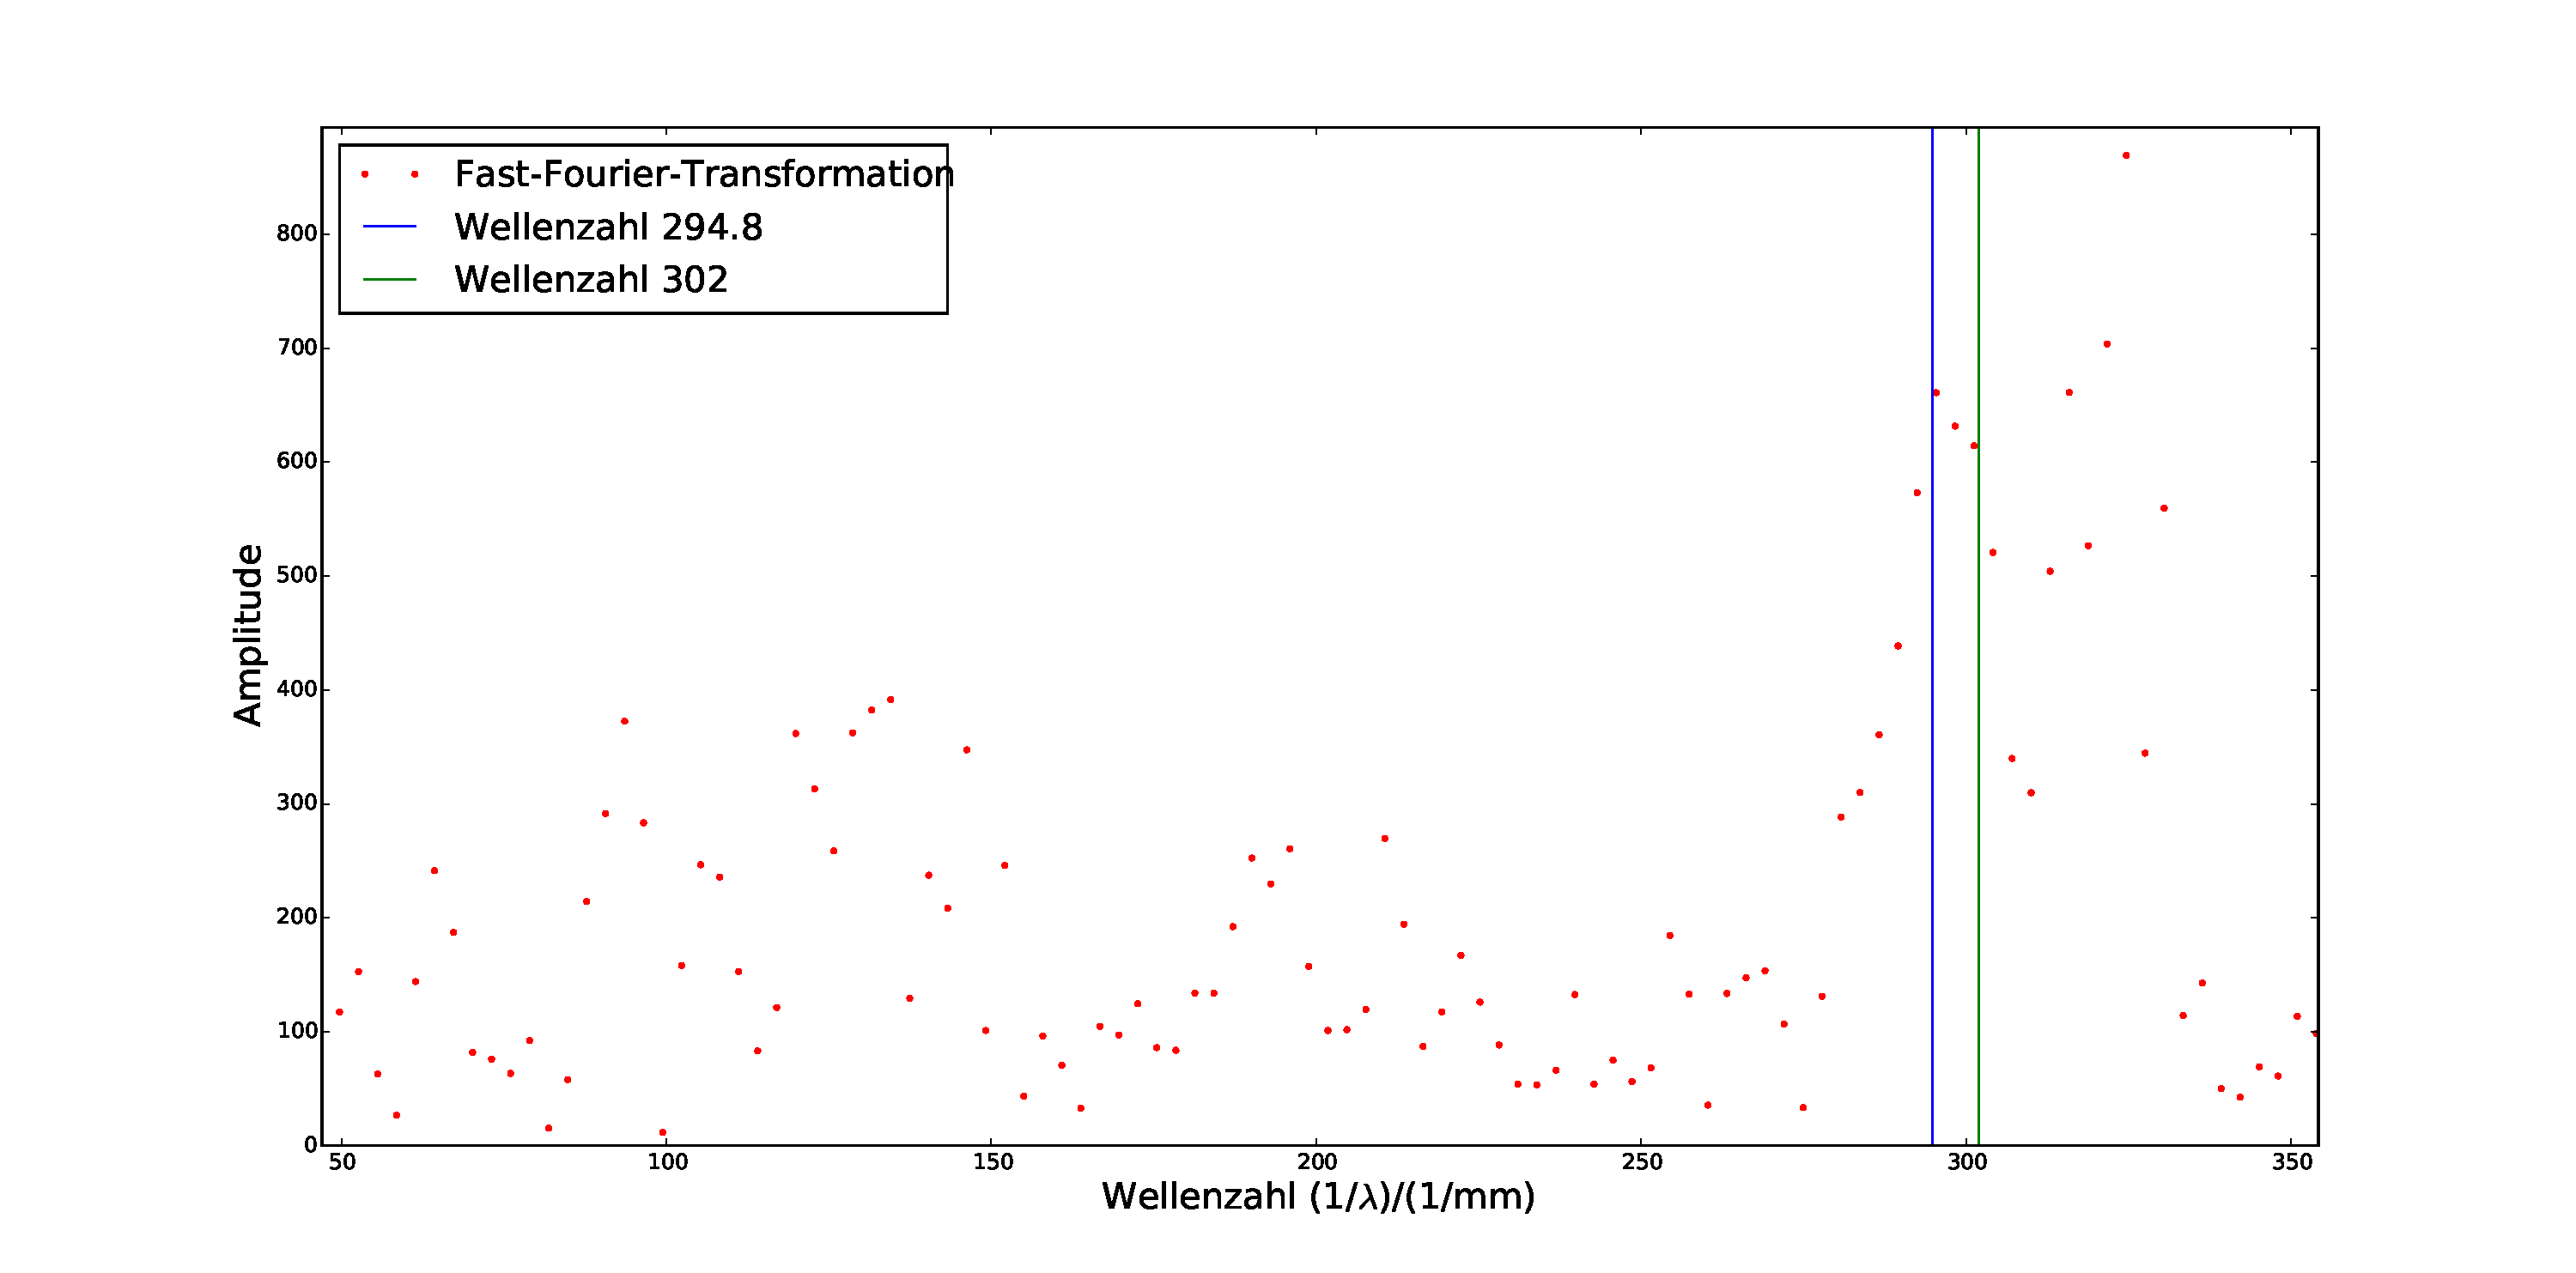
\includegraphics[scale = 0.38, clip = true, trim = 3cm 0cm 3cm 0cm]{Wellenzahlen50-350SchwebungmitFenster(0,5*(1-cos))}
\caption{Diskrete Fouriertransformation des Schwebungsinterferogramms f�r Wellenzahlen ($1/\lambda$) von \SI{50}{$\frac{1}{mm}$} bis \SI{360}{$\frac{1}{mm}$} mit Fensterfunktion $f(x)=(\frac{1-\cos(\frac{2 \pi x}{L})}{2})$}
\label{fig:fftschwebungsinterferogramm_k_1}
\end{figure}
\begin{figure}[H]
\begin{subfigure}[t]{0.49\textwidth}
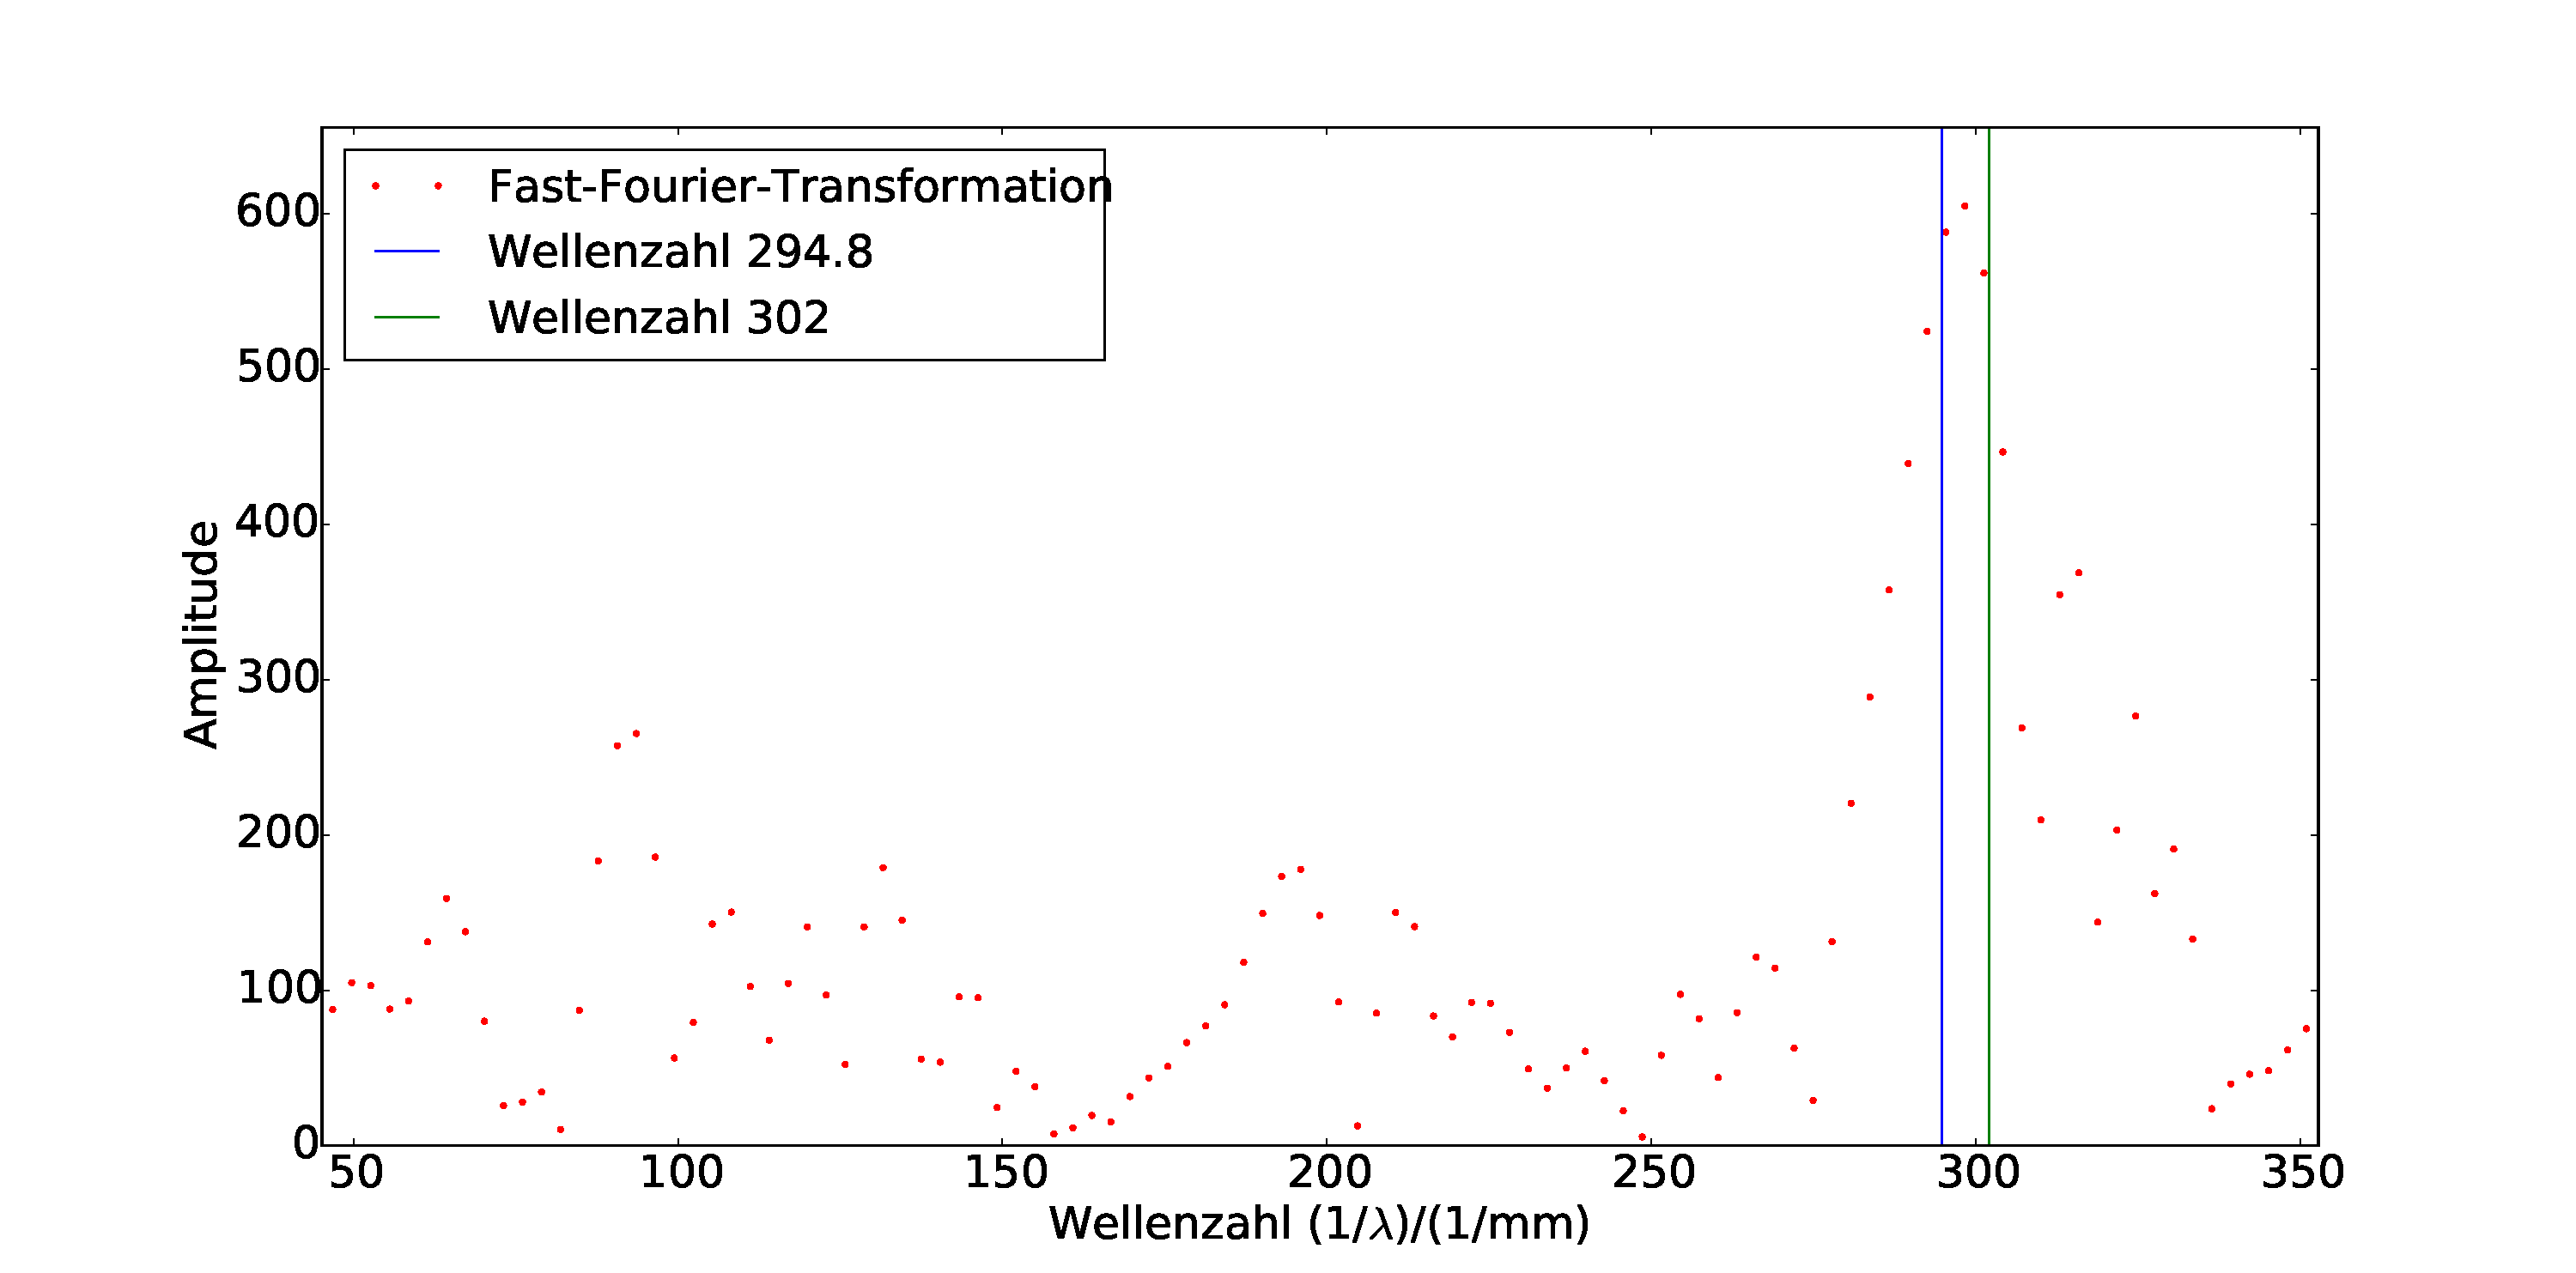
\includegraphics[scale = 0.19, clip = true, trim = 3cm 0cm 3cm 0cm]{Wellenzahlen50-350SchwebungmitFenster(0,5*(1-cos))**4}
\caption{Diskrete Fouriertransformation des Schwebungsinterferogramms f�r Wellenzahlen ($1/\lambda$) von \SI{50}{$\frac{1}{mm}$} bis \SI{360}{$\frac{1}{mm}$} mit Fensterfunktion\\$f(x)=(\frac{1-\cos(\frac{2 \pi x}{L})}{2})^4$}
\label{fig:fftschwebungsinterferogramm_k_4}
\end{subfigure}
\hspace{0.02\textwidth}
\begin{subfigure}[t]{0.49\textwidth}
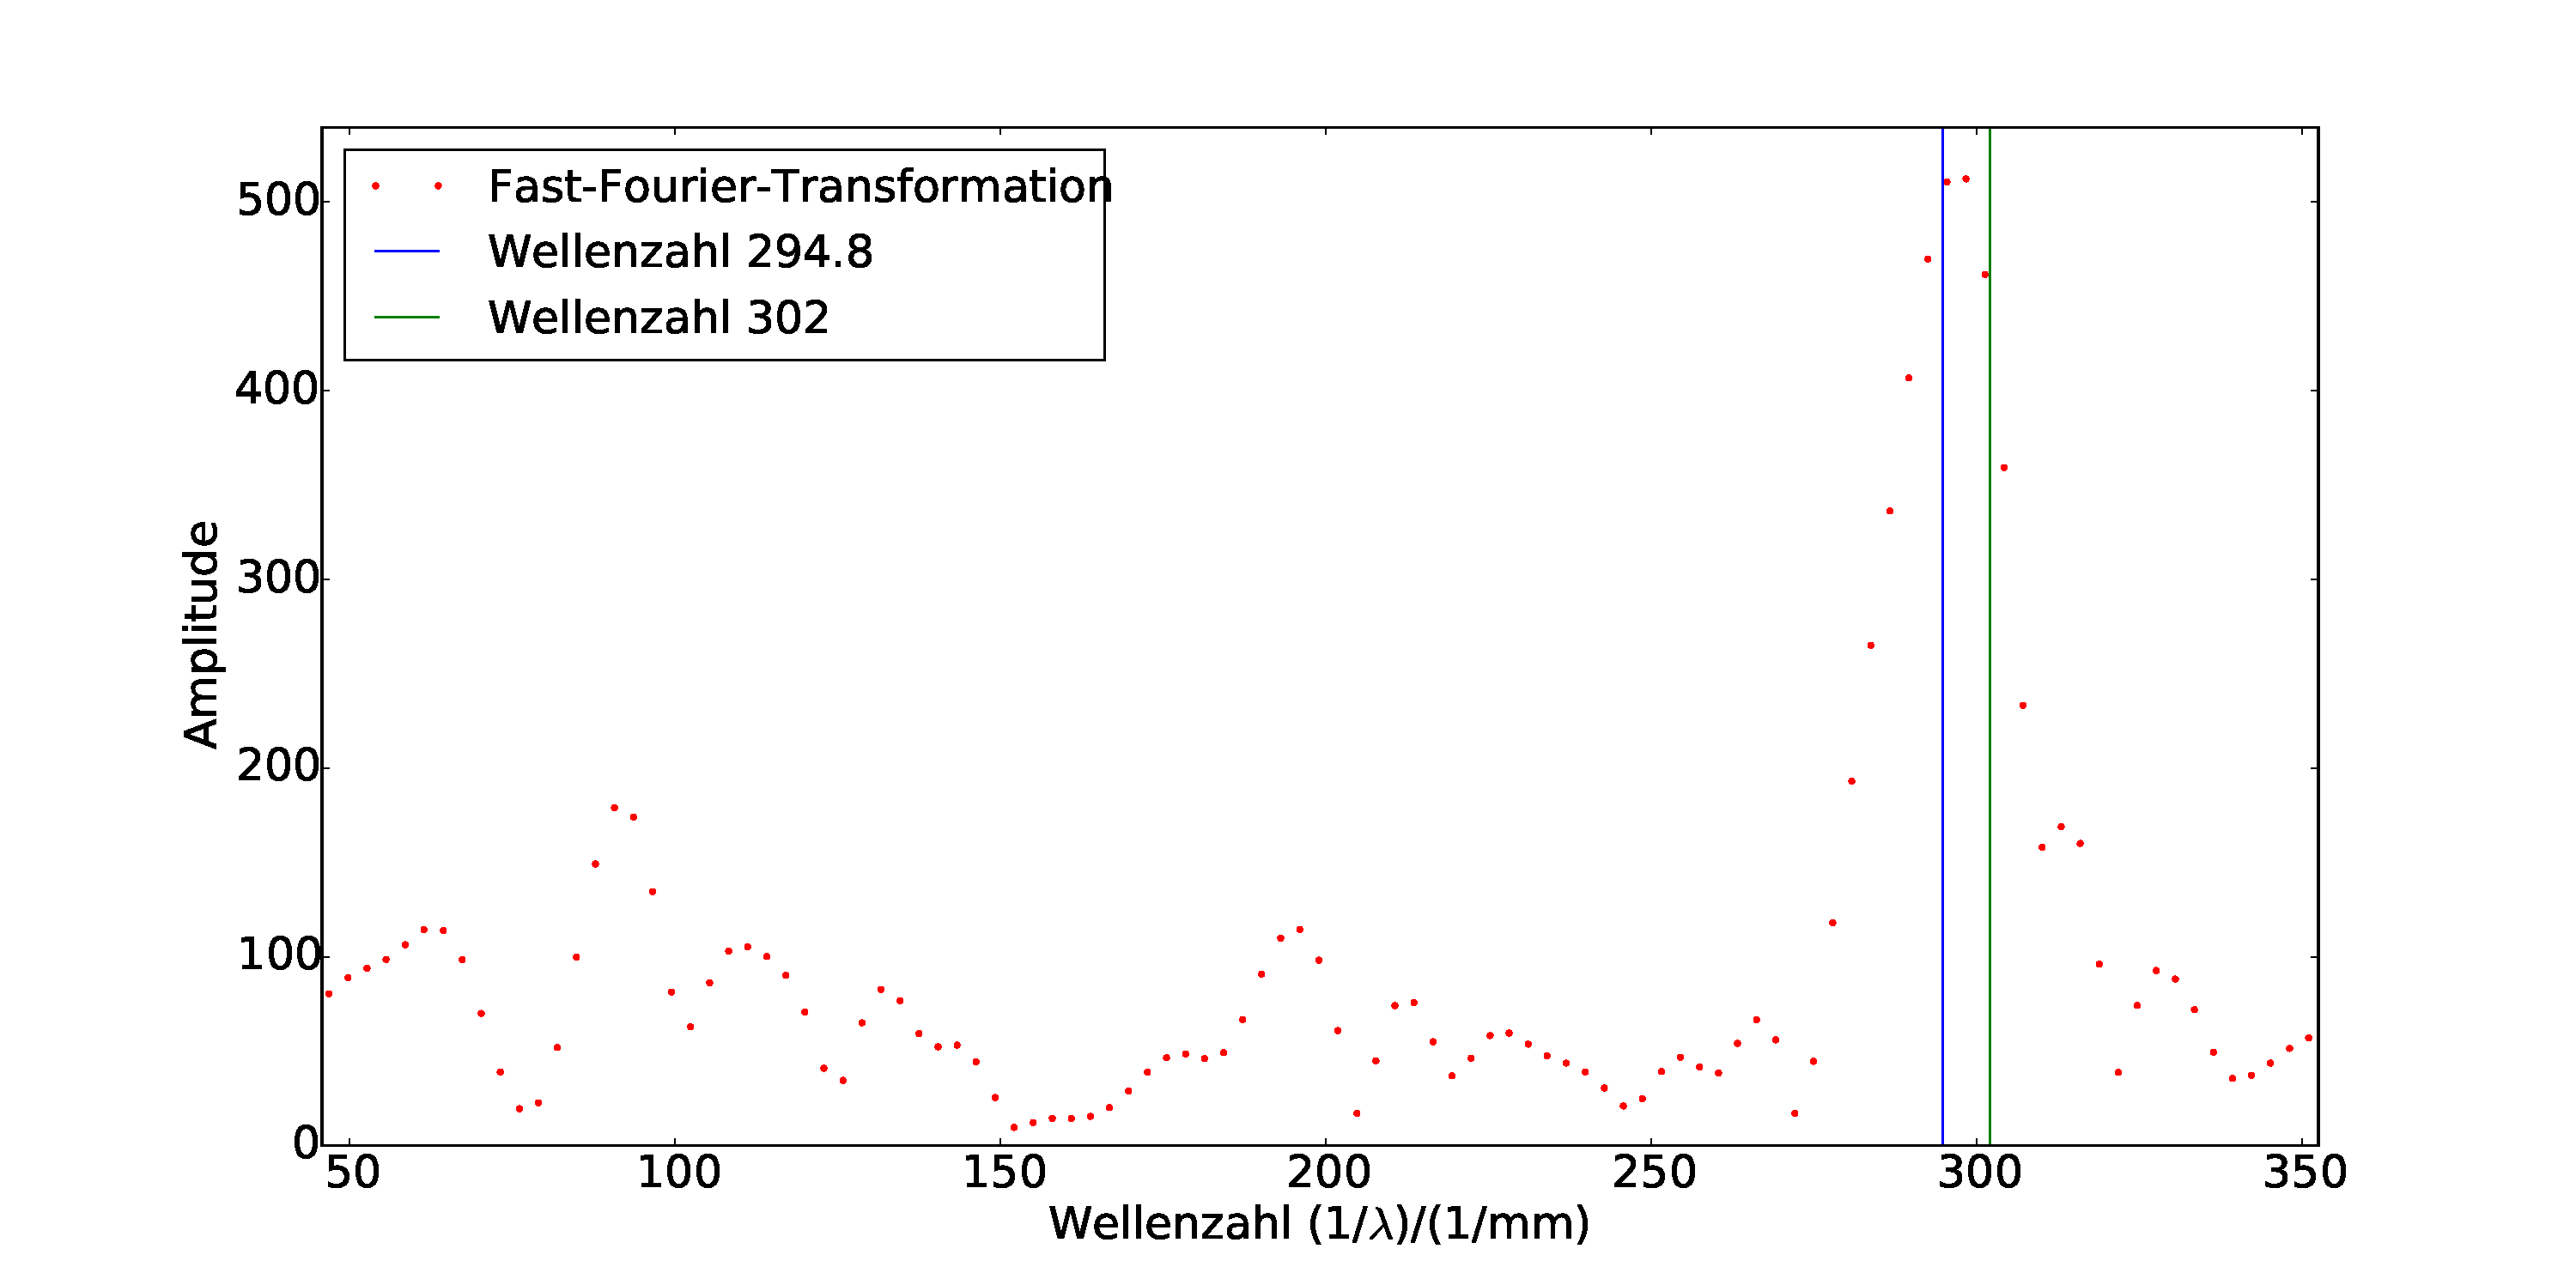
\includegraphics[scale = 0.19, clip = true, trim = 3cm 0cm 3cm 0cm]{Wellenzahlen50-350SchwebungmitFenster(0,5*(1-cos))**10}
\caption{Diskrete Fouriertransformation des Schwebungsinterferogramms f�r Wellenzahlen ($1/\lambda$) von \SI{50}{$\frac{1}{mm}$} bis \SI{360}{$\frac{1}{mm}$} mit Fensterfunktion\\$f(x)=(\frac{1-\cos(\frac{2 \pi x}{L})}{2})^{10}$}
\label{fig:fftschwebungsinterferogramm_k_10}
\end{subfigure}
\end{figure}
Man sieht, dass das Rauschen mit h�herem $k$ geringer wird, sodass die erwarteten Wellenzahlen bereits bei $k = 4$ die gr��te Amplitude im gesamten Interferogramm besitzen. Die beiden Peaks bei \SI{294,8(10)}{$\frac{1}{mm}$} und \SI{302(2)}{$\frac{1}{mm}$} verschmieren mit gr��er werdendem k zu einem Peak, sodass bei $k=10$ die Peaks nichtmehr voneinander unterschieden werden k�nnen. Trotzdem sieht man, dass das Rauschen bei $k=10$ am besten unterdr�ckt wird, sodass andere Wellenzahlen eine sehr geringe Amplitude besitzen. Daneben kann man Infrarotwellenzahlen von Plankstrahlern bei Raumtemperatur bei ca. \SI{100}{$\frac{1}{mm}$} in den letzten beiden Plots gut erkennen, welche ebenfalls nicht als Rauschen herausgefiltert werden. Diese Tatsache unterst�tzt die Konsistenz dieses Resultates. Zusammenfassend konnten die gefundenen Wellenl�ngen bei \SI{3,392(12)}{$\mu$m} und \SI{3,31(2)}{$\mu$m} per FFT mit relativ gro�er Genauigkeit durch die Benutzung von Fensterfunktionen bestimmt werden, wobei der Peak bei der Wellenl�nge \SI{3,31(2)}{$\mu$m} abh�ngig von der Fensterfunktion nicht mehr zu erkennen ist.

\subsubsection{Manuelle Auswertung der Schwebung}
Eine Manuelle Auswertung des Schwebungsinterferogramms wird trotz Schwierigkeiten so weit wie m�glich durchgef�hrt.
Die beiden Wellenl�ngen $\lambda_-$ und $\lambda_+$ werden wie zuvor bestimmt (vgl. \ref{sec:chopper}). F�r $\lambda_+$ ein Werte von 275,6(3) $\mu$m bestimmt, indem �ber eine 1/4-Periode gez�hlt wurde. F�r $\lambda_-$ wurde ein Wert von 3,15(3) $\mu$m bestimmt. Mit den zuvor bestimmten Wellenl�ngen des Muffelofen und des Lasers ergeben sich die Werte in Tabelle \ref{tab:wellenlaengen}.

\begin{table}[H]
\centering
\caption{Bestimmte Wellenl�ngen $\lambda_{Laser,Muffelofen,+,-}$}
\label{tab:wellenlaengen}
\begin{tabular}{|c|c|}
\hline $\lambda_{Laser}$ & \SI{3,372(9)}{$\mu$m} \\ 
\hline $\lambda_{Ofen}$ & \SI{2,91(5)}{$\mu$m} \\ 
\hline $\lambda_{+}$ & \SI{275,6(3)}{$\mu$m} \\ 
\hline $\lambda_{-}$ & \SI{3,15(3)}{$\mu$m} \\ 
\hline 
\end{tabular} 
\end{table}
Die Parameter $2\pi b_{Laser}$ und $2\pi b_{Ofen}$ werden wie in Abschnitt \ref{sec:filter} bestimmt, der Parameter $a$ wird �bernommen. Es ergeben sich die Werte in Tabelle \ref{tab:parameter_2}.

\begin{table}[H]
\centering
\caption{Parameter f�r die spektrale Verteilung}
\label{tab:parameter_2}
\begin{tabular}{|c|c|}
\hline $a$ & 0,0129(1) mm \\ 
\hline $2\pi b_{Laser}$ & \SI{1,863(5)}{$\mu$m} \\
\hline $2\pi b_{Ofen}$ & \SI{2,159(37)}{$\mu$m} \\
\hline 
\end{tabular} 
\end{table}

Mit den Werten aus Tabelle \ref{tab:parameter_2} ergibt sich die spektrale Verteilung in Abbildung \ref{fig:spektrum_schwebung}.

\begin{figure}[H]
\centering
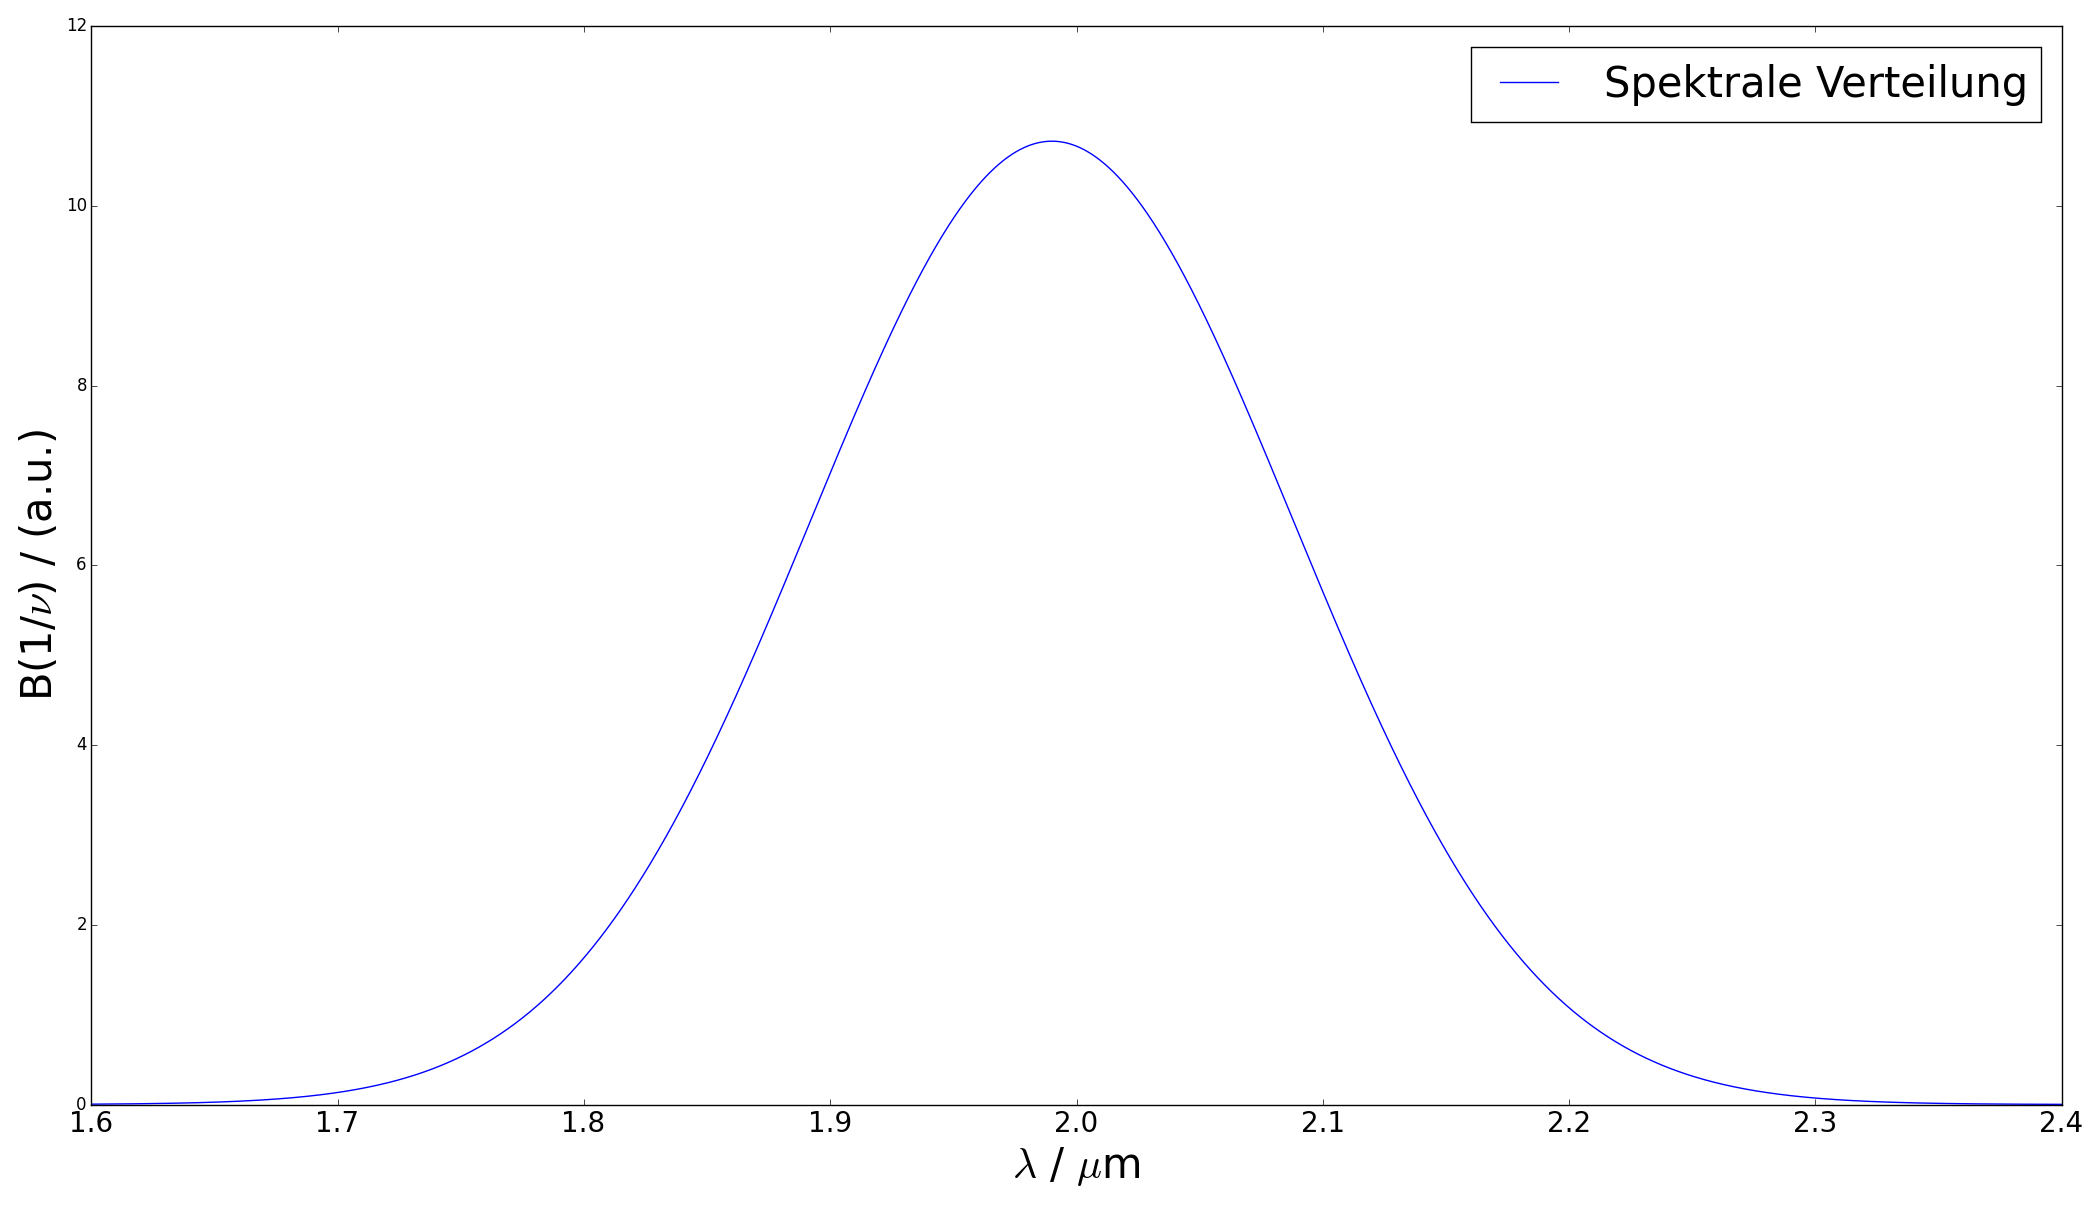
\includegraphics[scale = 0.33]{verteilung_schwebung.png}
\caption{Spektrale Verteilung der Schwebung}
\label{fig:spektrum_schwebung}
\end{figure}
\section{Conclusion}
%im fazit nochmal alles zusammenfassen und den verlauf der messung absch�tzen
%gravierende sytematische probleme bei den messungen nochmal betonen und die wertigkeit unserer ergebnisse einordnen

In the first part of the experiment the 39 peaks of the nH$_3$ spectrum where measured and there relative absorption coefficients where calculated. In the second part the quadrupole moment where determined with a value of 5.02(9), with a deviation of 17.53\%. In the last part the broadening of the peaks according to the pressure was determined with 28 witch is a good measurement. 
\newpage
\appendix
\section{Kalibrierung}
\label{sec:kalib_anhang}

\begin{figure}[H]
\centering
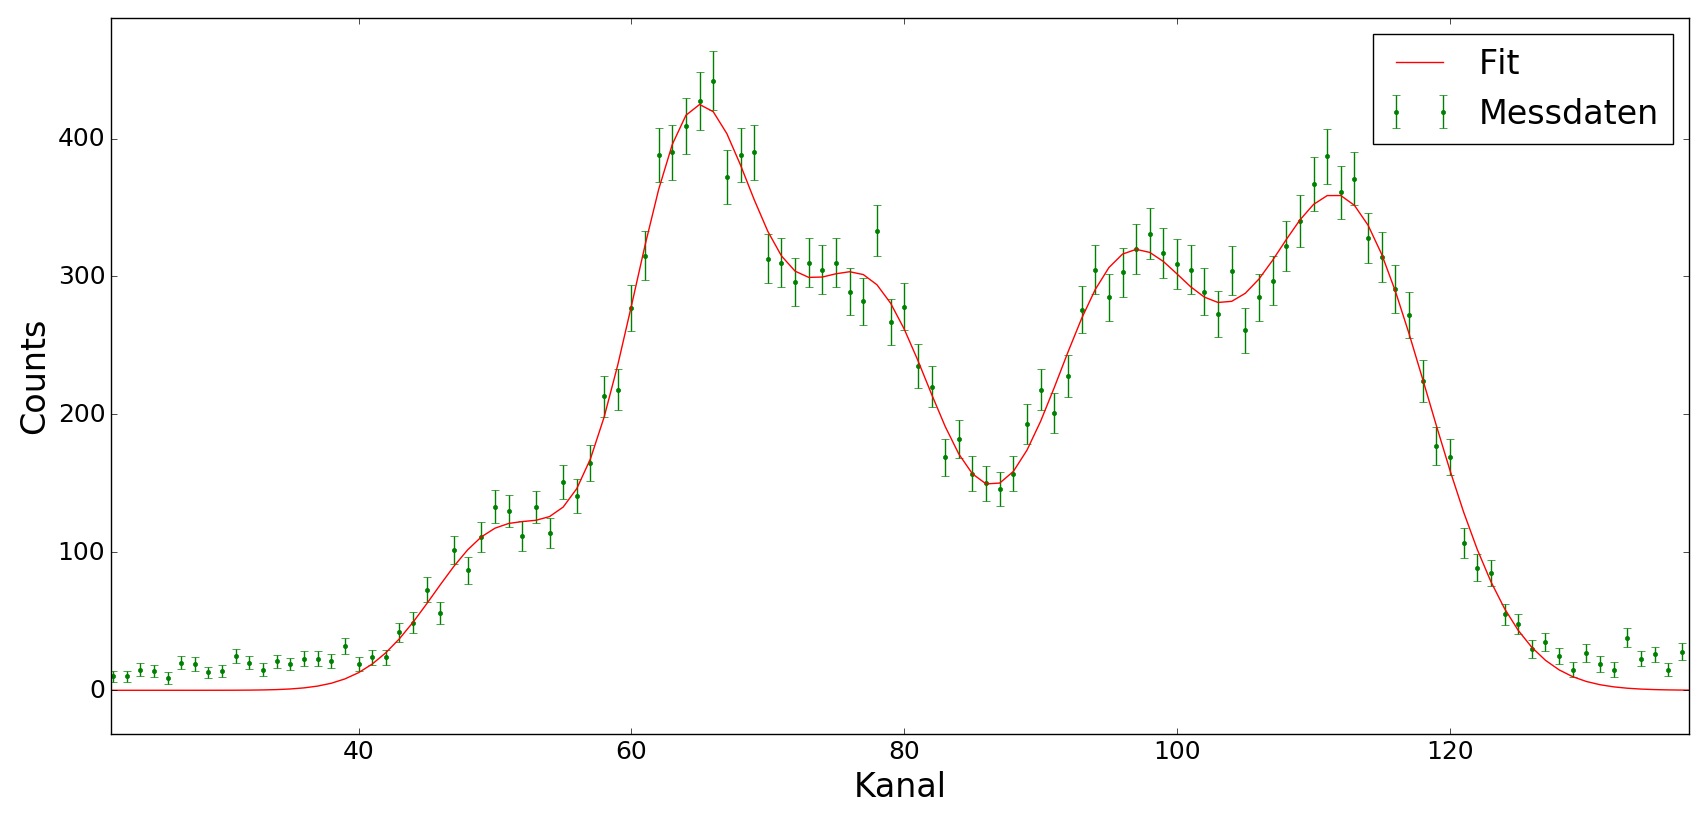
\includegraphics[scale = 0.39]{kalib_fit_1.png}
\caption{Fit der vorderen Peaks f�r $^{241}$Am. Die Fitparameter sind in Tabelle \ref{tab:kalib_fit_1} eingetragen.}
\label{fig:kilb_fit_1}
\end{figure}

\begin{table}[H]
\centering
\caption{Fitparameter f�r die vorderen Peaks der $^{241}$Am Quelle. Das $\chi^2_{red}$ ergab sich mit 1,15}
\label{tab:kalib_fit_1}
\begin{tabular}{|c|c|c|}
\hline Gau�peak & Parameter & Wert \\ 
\hline 1 & Amplitude & 1422(173) \\ 
\hline  & Center & 50,5(7) \\ 
\hline  & Sigma & 5,0(4) \\ 
\hline 2 & Amplitude & 4871(649) \\ 
\hline  & Center & 64,5(5) \\ 
\hline  & Sigma & 4,8(4) \\ 
\hline 3 & Amplitude & 3939(652) \\ 
\hline  & Center & 77,3(7) \\ 
\hline  & Sigma & 5,5(7) \\ 
\hline 4 & Amplitude & 4451(427) \\ 
\hline  & Center & 96,2(4) \\ 
\hline  & Sigma & 5,9(5) \\ 
\hline 5 & Amplitude & 5577(315) \\ 
\hline  & Center & 112,0(4) \\ 
\hline  & Sigma & 6,3(2) \\ 
\hline 
\end{tabular} 
\end{table}


\begin{figure}[H]
\centering
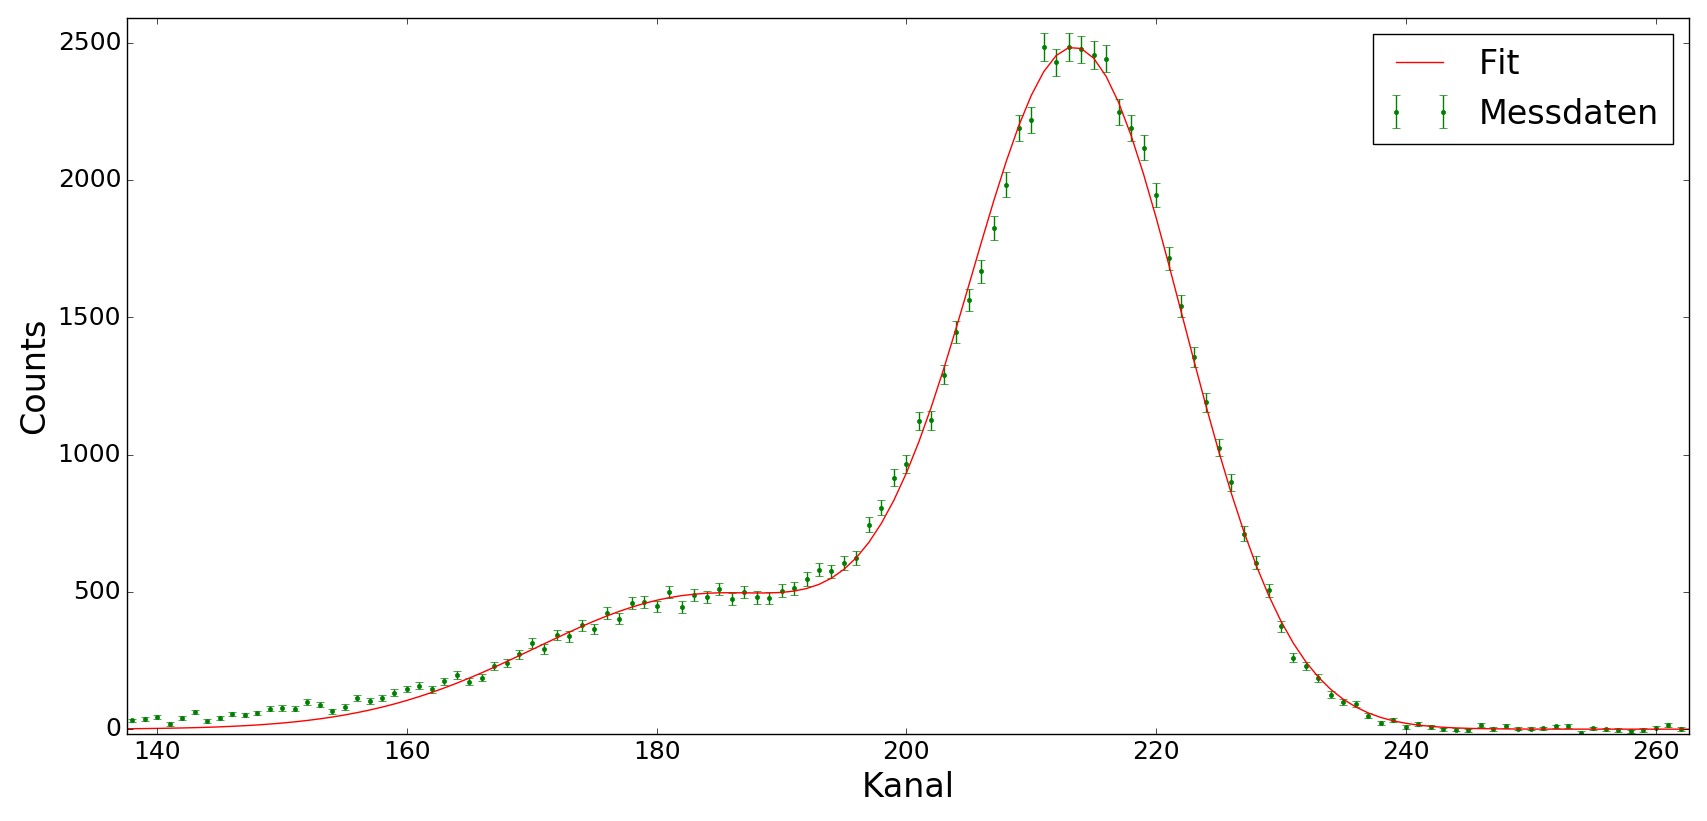
\includegraphics[scale = 0.39]{kalib_fit_2.png}
\caption{Fit des Hauptpeaks f�r $^{241}$Am. Die Fitparameter sind in Tabelle \ref{tab:kalib_fit_2} eingetragen. Das $\chi^2_{red}$ ergab sich mit 1,67}
\label{fig:kalib_fit_2}
\end{figure}

\begin{table}[H]
\centering
\caption{Fitparameter f�r die vorderen Peaks der $^{241}$Am Quelle.}
\label{tab:kalib_fit_2}
\begin{tabular}{|c|c|c|}
\hline Gau�peak & Parameter & Wert \\ 
\hline 1 & Amplitude & 16761(654) \\ 
\hline  & Center & 184(6) \\ 
\hline  & Sigma & 13.7(6) \\ 
\hline 2 & Amplitude & 52316(604) \\ 
\hline  & Center & 213.6(1) \\ 
\hline  & Sigma & 8.56(7) \\ 
\hline 
\end{tabular} 
\end{table}


\begin{figure}[H]
\centering
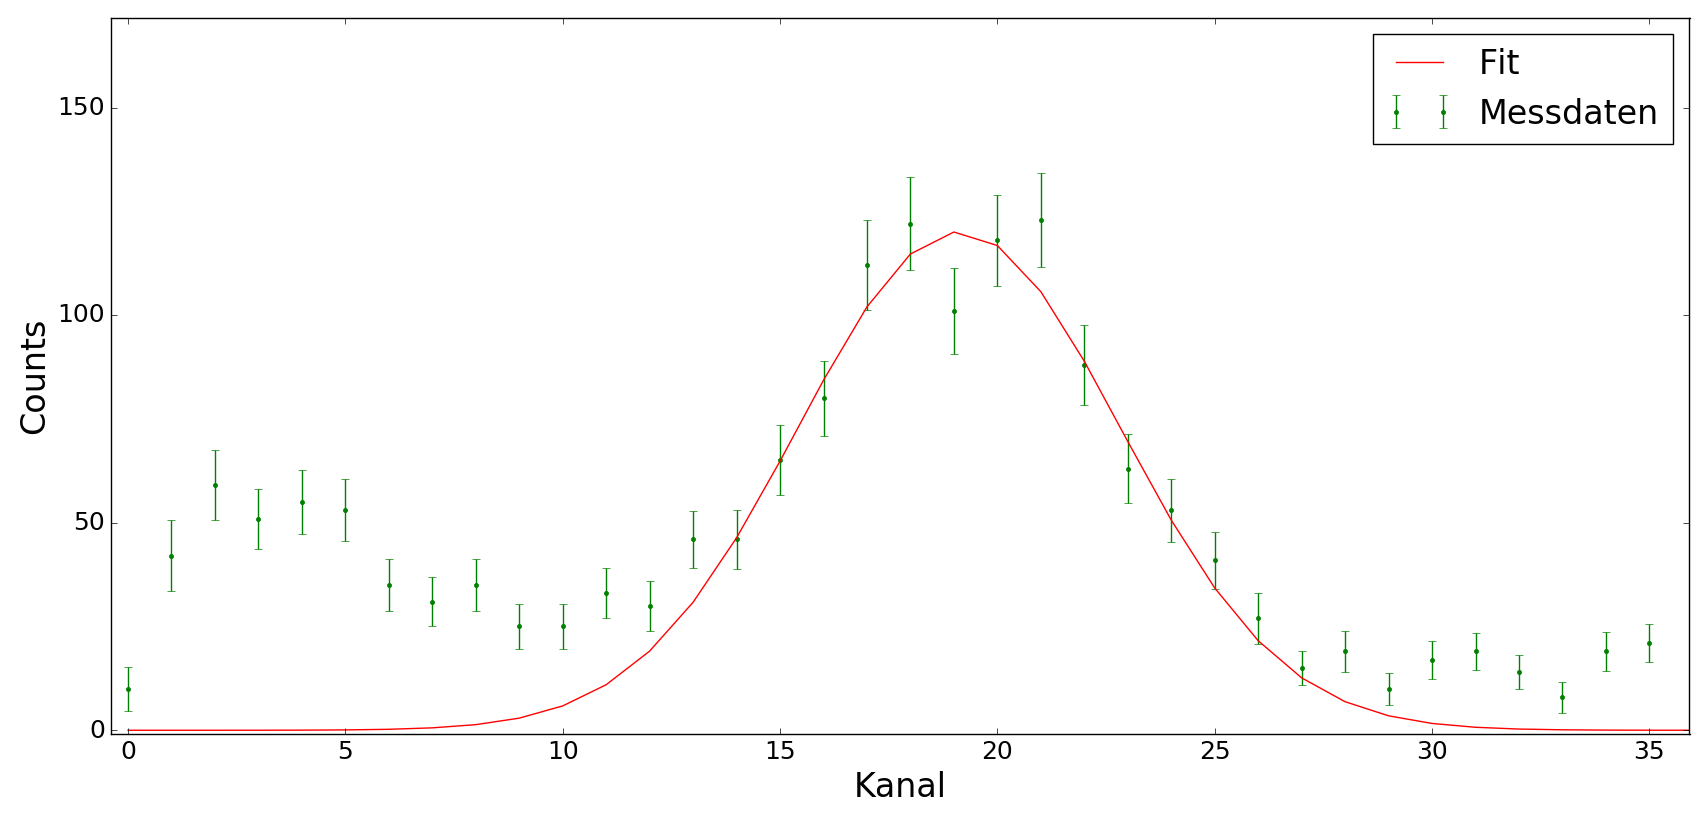
\includegraphics[scale = 0.39]{kalib_fit_3.png}
\caption{Fit des ersten Peaks f�r $^{133}$Ba. Die Fitparameter sind in Tabelle \ref{tab:kalib_fit_3} eingetragen.}
\label{fig:kilb_fit_3}
\end{figure}

\begin{table}[H]
\centering
\caption{Fitparameter f�r die vorderen Peaks der $^{133}$Ba Quelle. Das $\chi^2_{red}$ ergab sich mit 1,14}
\label{tab:kalib_fit_3}
\begin{tabular}{|c|c|c|}
\hline Gau�peak & Parameter & Wert \\ 
\hline 1 & Amplitude & 1118(61) \\ 
\hline  & Center & 19.1(2) \\ 
\hline  & Sigma & 3.7(3) \\ 
\hline 
\end{tabular} 
\end{table}


\begin{figure}[H]
\centering
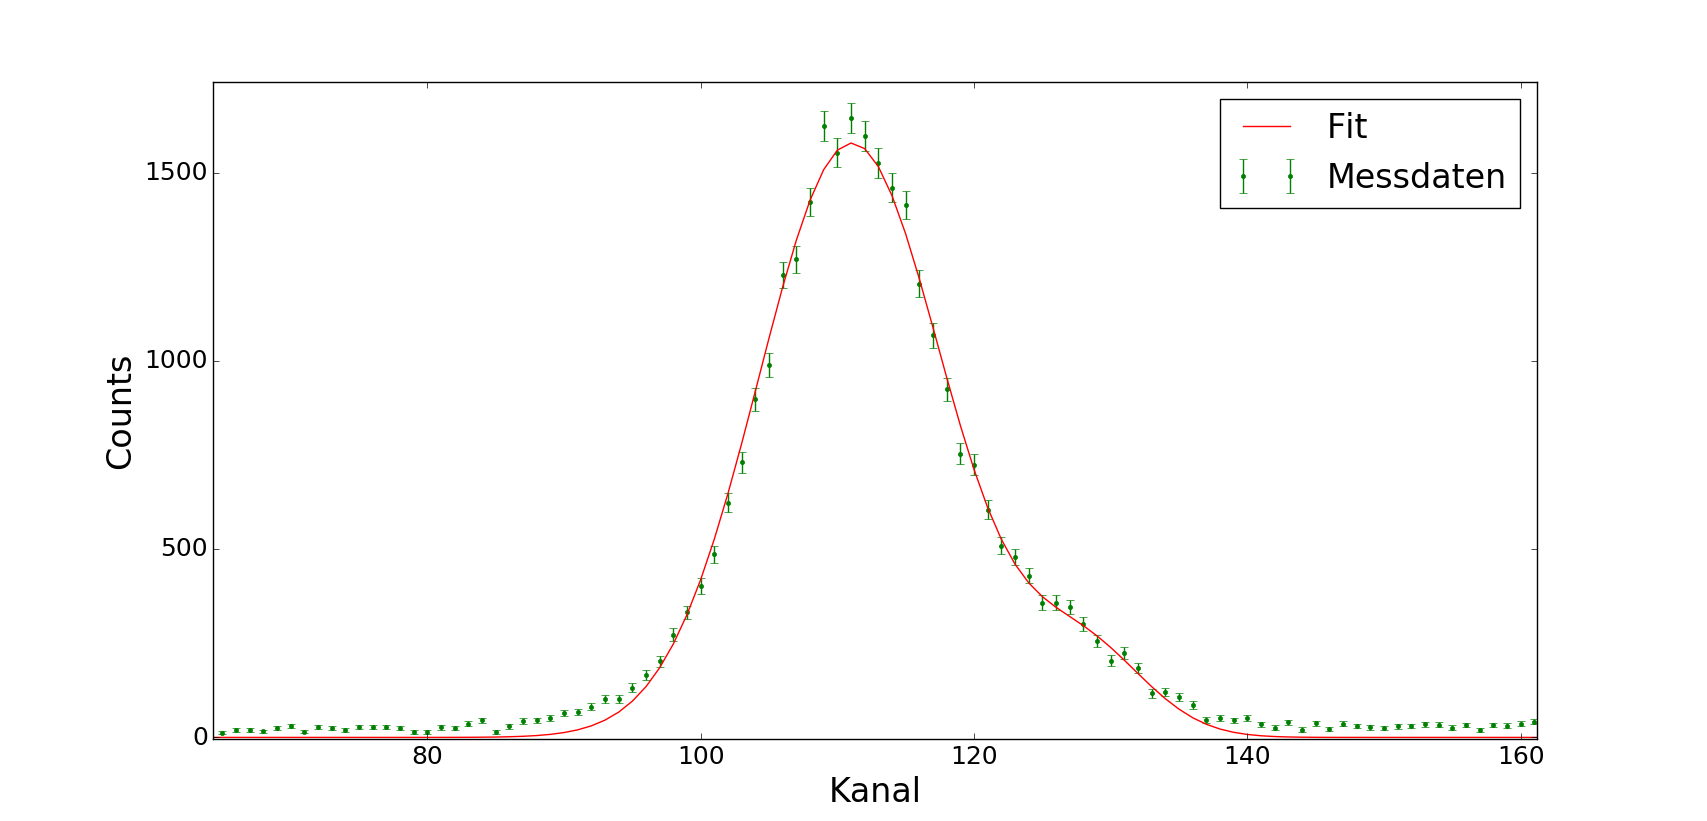
\includegraphics[scale = 0.39]{kalib_fit_4.png}
\caption{Fit des zweiten Peaks f�r $^{133}$Ba. Die Fitparameter sind in Tabelle \ref{tab:kalib_fit_4} eingetragen.}
\label{fig:kilb_fit_4}
\end{figure}

\begin{table}[H]
\centering
\caption{Fitparameter f�r den zweiten Peak der $^{133}$Ba Quelle. Das $\chi^2_{red}$ ergab sich mit 2.31}
\label{tab:kalib_fit_4}
\begin{tabular}{|c|c|c|}
\hline Gau�peak & Parameter & Wert \\ 
\hline 1 & Amplitude & 26864(382) \\ 
\hline  & Center & 111.1(1) \\ 
\hline  & Sigma & 6.8(1) \\ 
\hline 2 & Amplitude & 2615(323) \\ 
\hline  & Center & 128(5) \\ 
\hline  & Sigma & 4.5(5) \\ 
\hline 
\end{tabular} 
\end{table}



\begin{figure}[H]
\centering
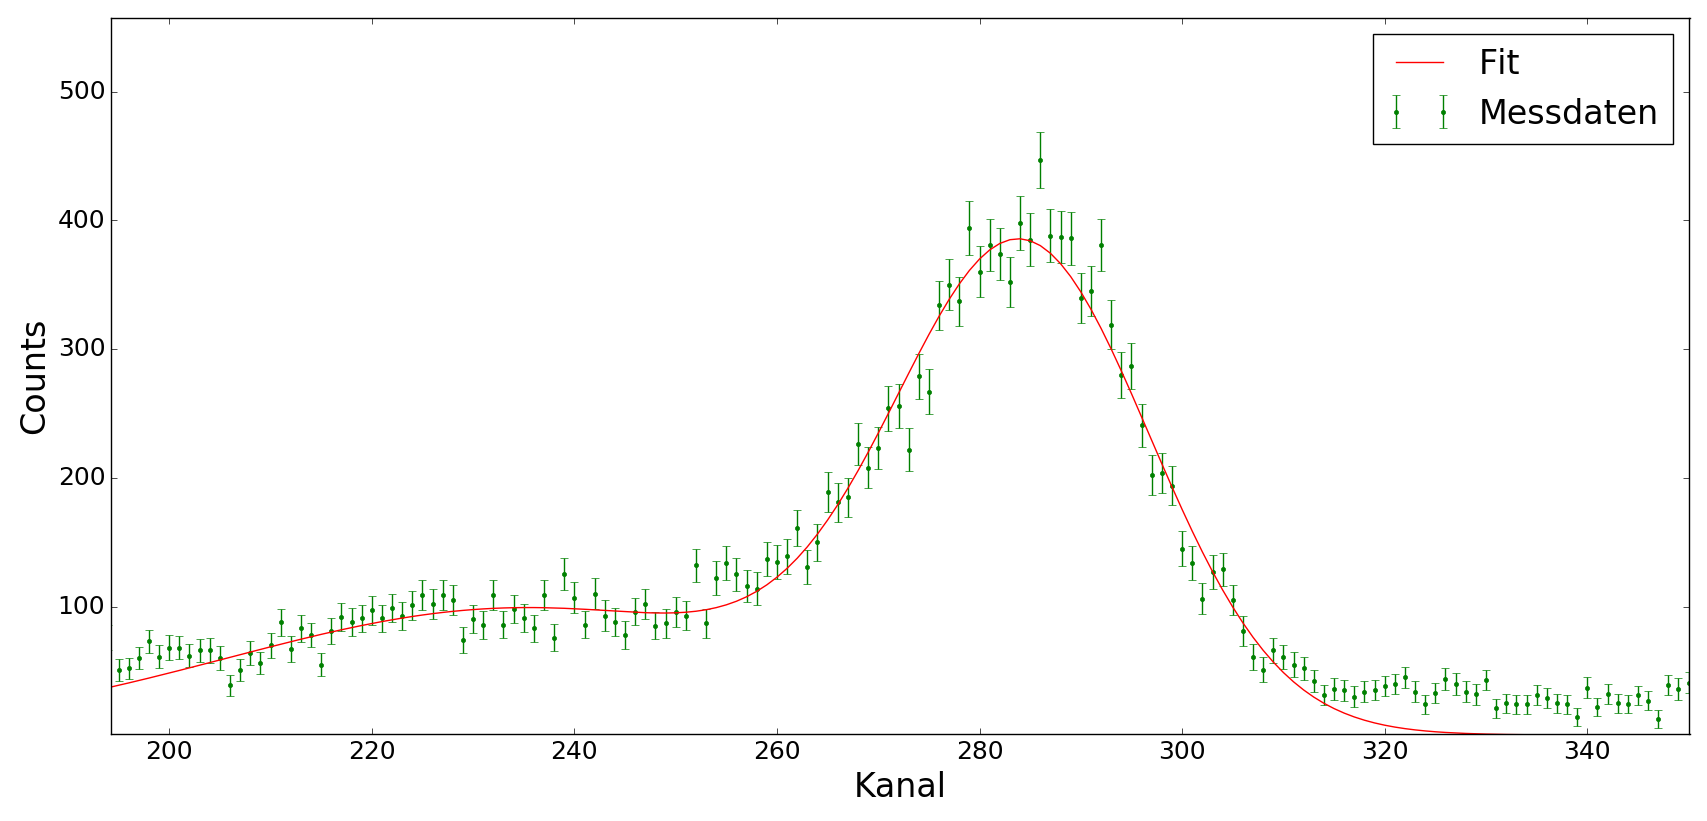
\includegraphics[scale = 0.39]{kalib_fit_5.png}
\caption{Fit des dritten Peaks f�r $^{133}$Ba. Die Fitparameter sind in Tabelle \ref{tab:kalib_fit_5} eingetragen.}
\label{fig:kilb_fit_5}
\end{figure}

\begin{table}[H]
\centering
\caption{Fitparameter f�r die dritten Peaks der $^{133}$Ba Quelle. Das $\chi^2_{red}$ ergab sich mit 1.77}
\label{tab:kalib_fit_5}
\begin{tabular}{|c|c|c|}
\hline Gau�peak & Parameter & Wert \\ 
\hline 1 & Amplitude & 7263(781) \\ 
\hline  & Center & 235(5) \\ 
\hline  & Sigma & 29(4) \\ 
\hline 2 & Amplitude & 11357(560) \\ 
\hline  & Center & 284.4(3) \\ 
\hline  & Sigma & 12.5(3) \\ 
\hline 
\end{tabular} 
\end{table}



\begin{figure}[H]
\centering
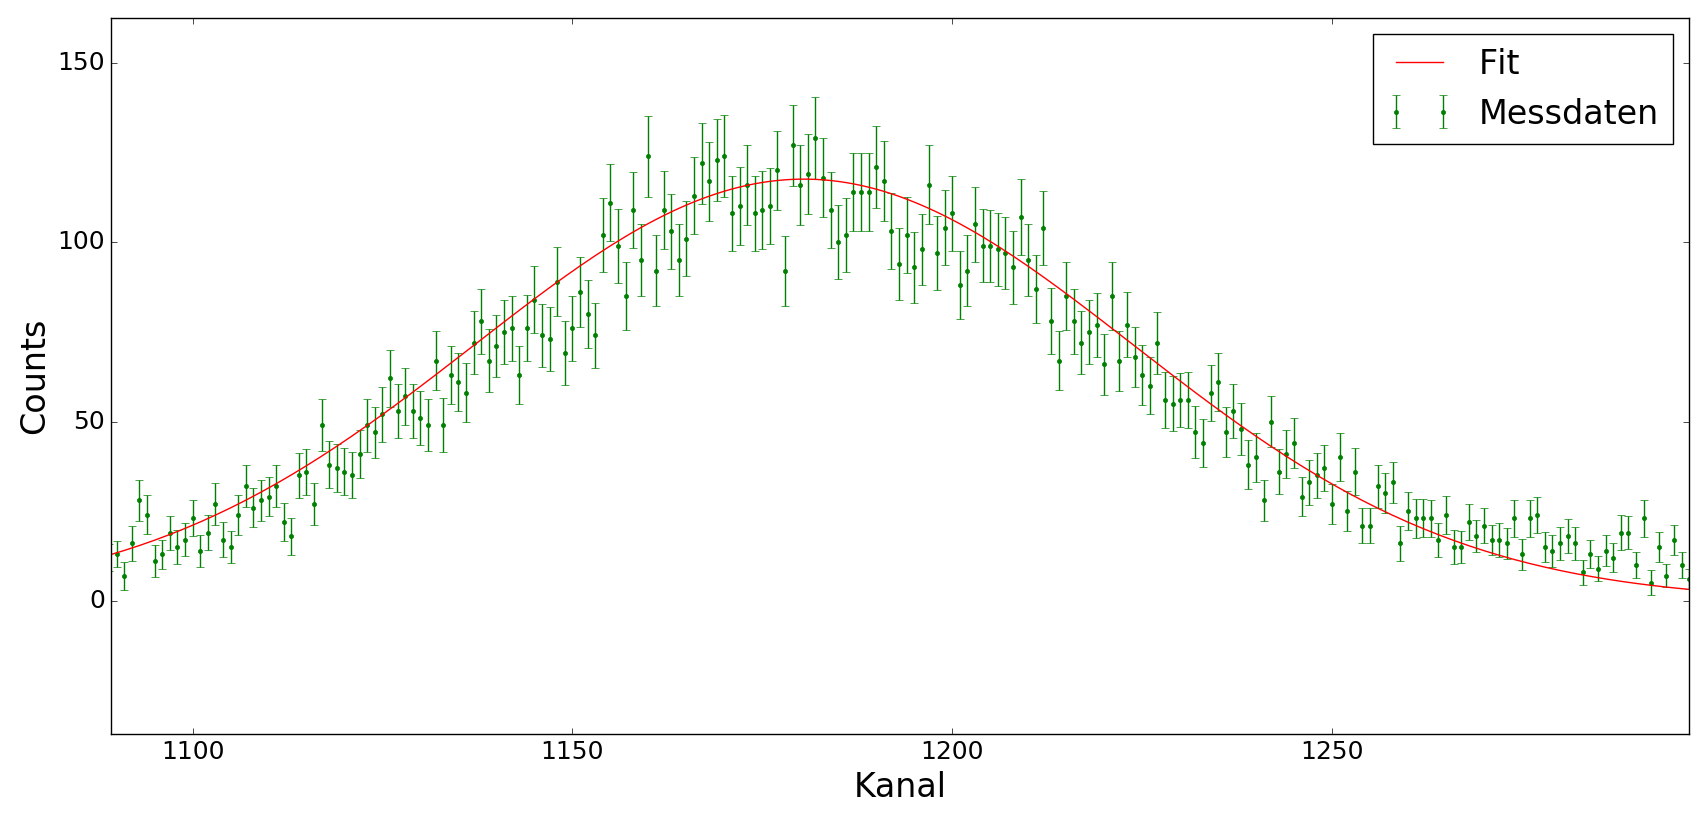
\includegraphics[scale = 0.39]{kalib_fit_6.png}
\caption{Fit des vierten Peaks f�r $^{133}$Ba. Die Fitparameter sind in Tabelle \ref{tab:kalib_fit_6} eingetragen.}
\label{fig:kilb_fit_6}
\end{figure}

\begin{table}[H]
\centering
\caption{Fitparameter des vierten Peaks der $^{133}$Ba Quelle. Das $\chi^2_{red}$ ergab sich mit 0,80}
\label{tab:kalib_fit_6}
\begin{tabular}{|c|c|c|}
\hline Gau�peak & Parameter & Wert \\ 
\hline 1 & Amplitude & 12789(117) \\ 
\hline  & Center & 1180,5(5) \\ 
\hline  & Sigma & 43,4(5) \\ 
\hline 
\end{tabular} 
\end{table}


\begin{figure}[H]
\centering
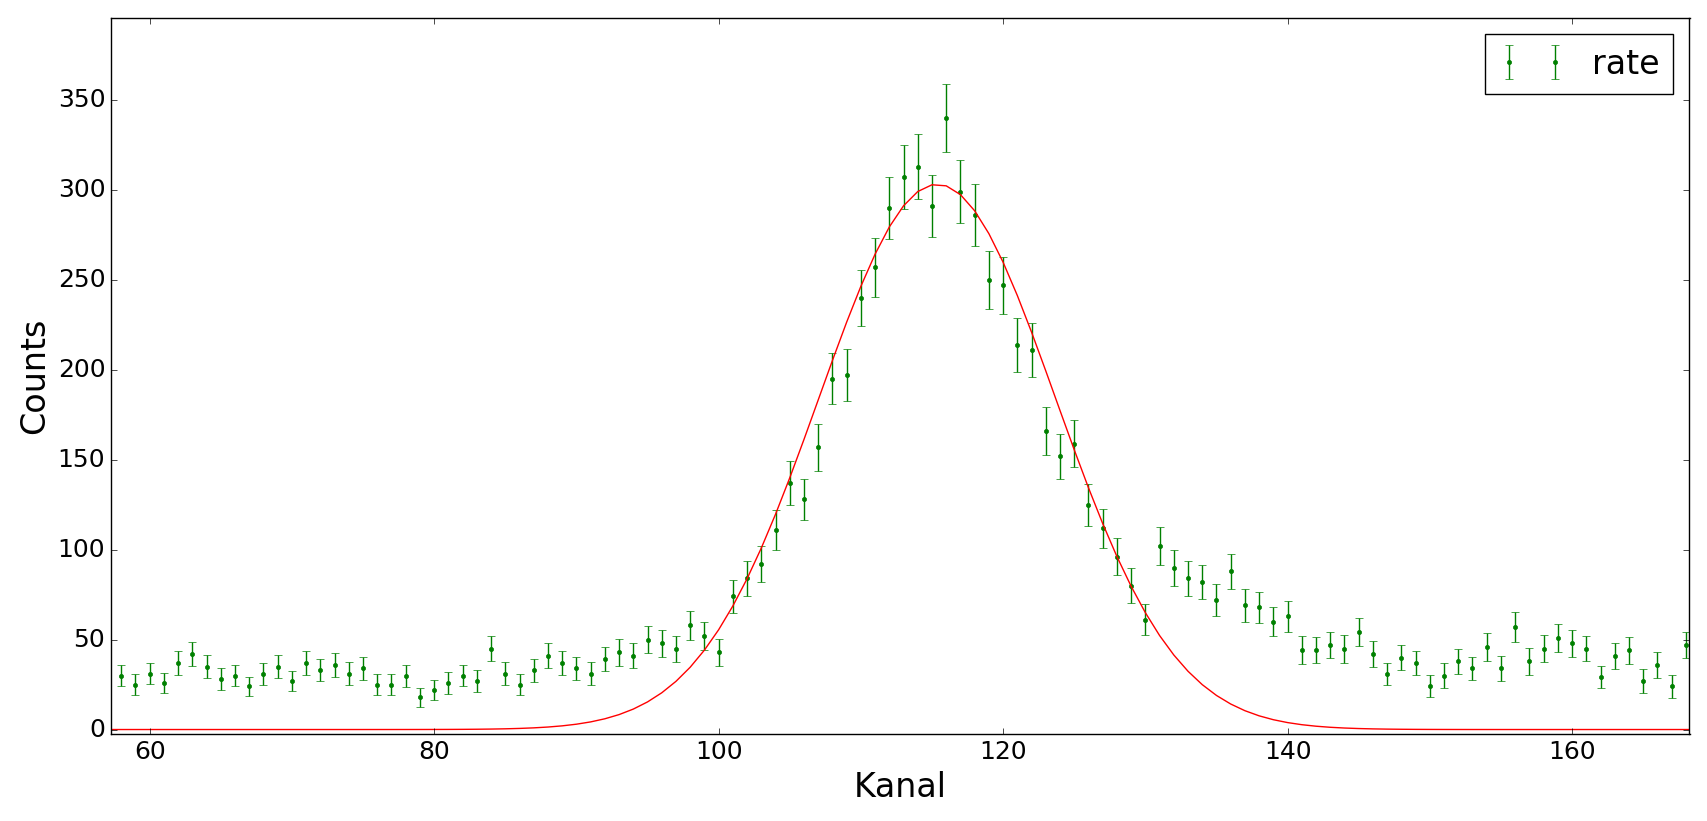
\includegraphics[scale = 0.39]{kalib_fit_7.png}
\caption{Fit des ersten Peaks f�r $^{137}$Cs. Die Fitparameter sind in Tabelle \ref{tab:kalib_fit_7} eingetragen.}
\label{fig:kilb_fit_7}
\end{figure}

\begin{table}[H]
\centering
\caption{Fitparameter des ersten Peaks der $^{137}$Cs Quelle. Das $\chi^2_{red}$ ergab sich mit 1,34}
\label{tab:kalib_fit_7}
\begin{tabular}{|c|c|c|}
\hline Gau�peak & Parameter & Wert \\ 
\hline 1 & Amplitude & 6336(103) \\ 
\hline  & Center & 115,5(2) \\ 
\hline  & Sigma & 8,3(2) \\ 
\hline 
\end{tabular} 
\end{table}

\section{Absorption}
\label{sec:absorption_anhang}

\subsection{Blei}


\begin{figure}[H]
\centering
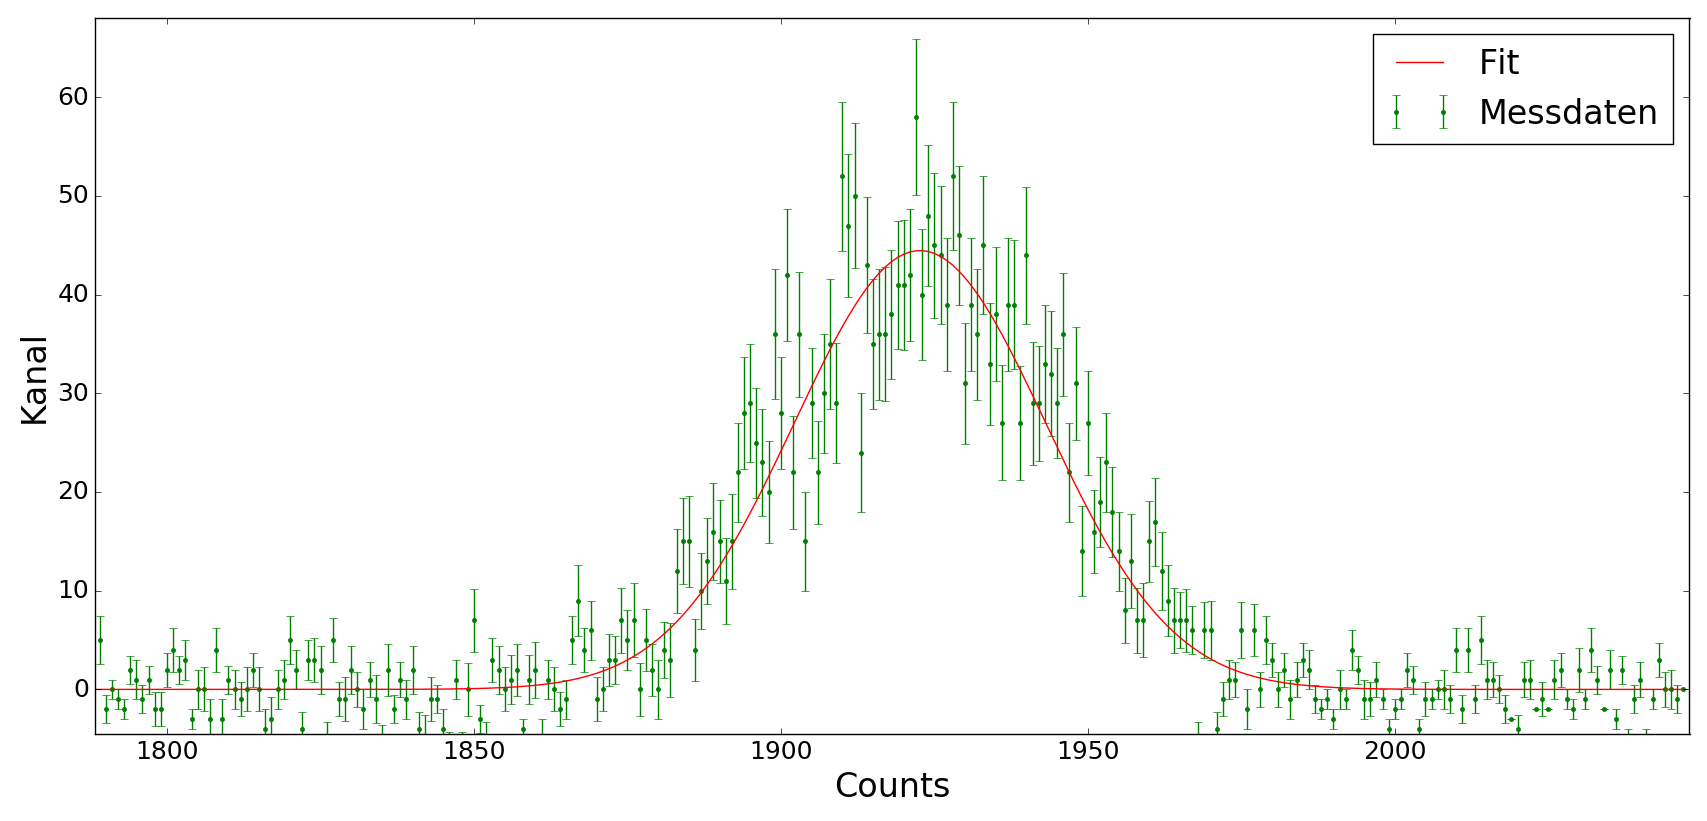
\includegraphics[scale = 0.39]{absrop_fit_blei_1.png}
\caption{Fit des Peaks mit 7,06cm Blei. Die Fitparameter sind in Tabelle \ref{tab:absorp_fit_1} eingetragen.}
\label{fig:absorp_fit_1}
\end{figure}

\begin{table}[H]
\centering
\caption{Fitparameter des Peaks mit 7,06cm Blei. Das $\chi^2_{red}$ ergab sich mit 2,03}
\label{tab:absorp_fit_1}
\begin{tabular}{|c|c|c|}
\hline Gau�peak & Parameter & Wert \\ 
\hline 1 & Amplitude & 2284(77) \\ 
\hline  & Center & 1922,7(7) \\ 
\hline  & Sigma & 20,5(6) \\ 
\hline 
\end{tabular} 
\end{table}


\begin{figure}[H]
\centering
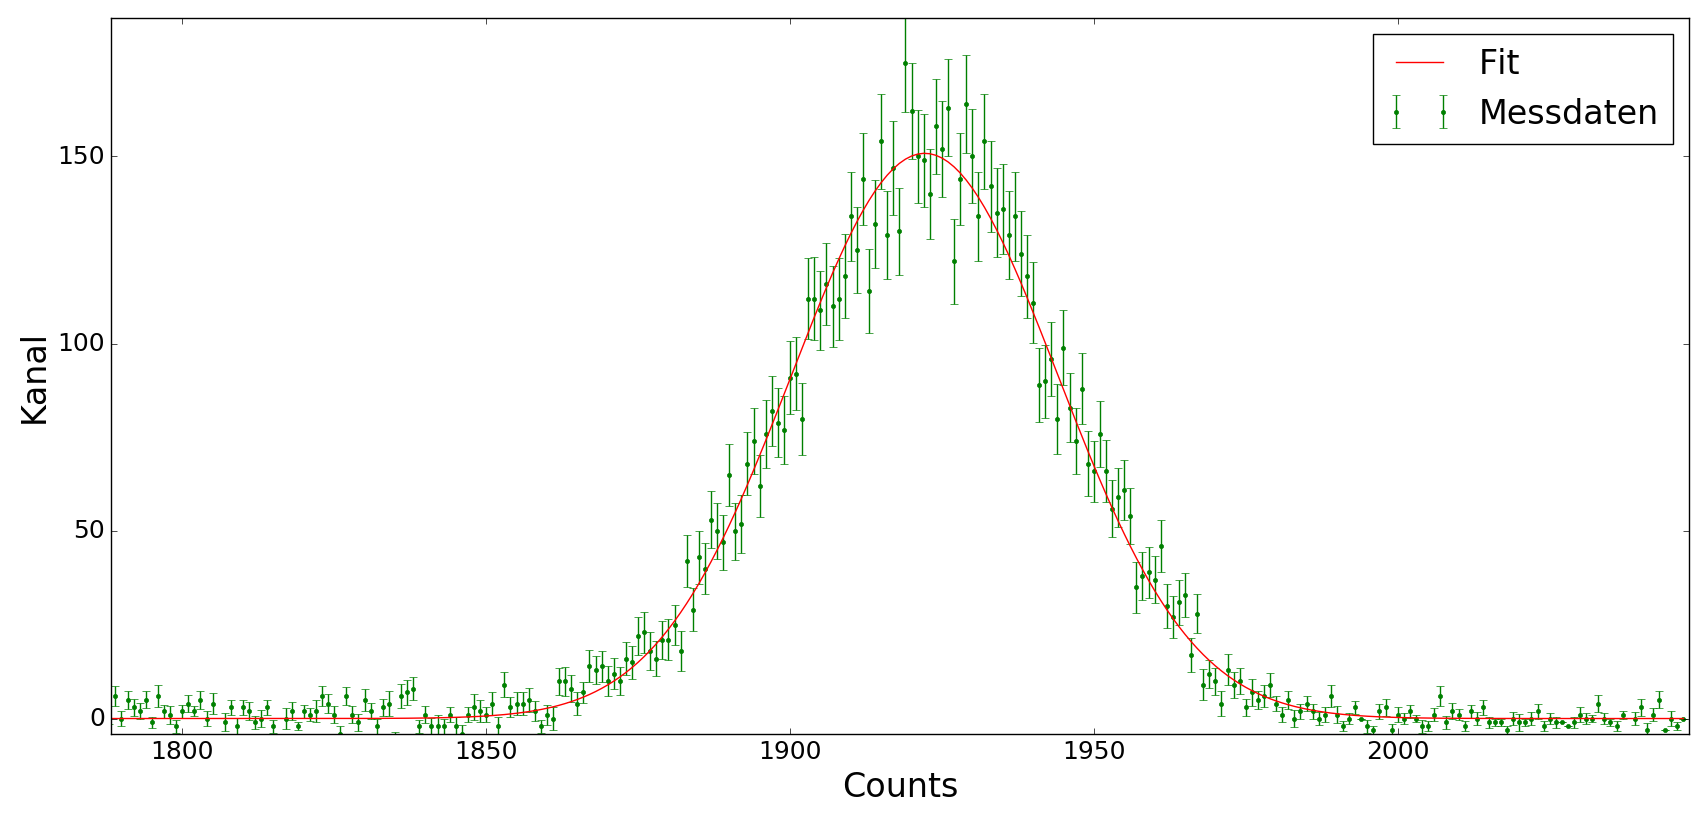
\includegraphics[scale = 0.39]{absrop_fit_blei_2.png}
\caption{Fit des Peaks mit 6,03cm Blei. Die Fitparameter sind in Tabelle \ref{tab:absorp_fit_2} eingetragen.}
\label{fig:absorp_fit_2}
\end{figure}

\begin{table}[H]
\centering
\caption{Fitparameter des Peaks mit 6,03cm Blei. Das $\chi^2_{red}$ ergab sich mit 1,15}
\label{tab:absorp_fit_2}
\begin{tabular}{|c|c|c|}
\hline Gau�peak & Parameter & Wert \\ 
\hline 1 & Amplitude & 8299(101) \\ 
\hline  & Center & 1922,2(3) \\ 
\hline  & Sigma & 22,0(2) \\ 
\hline 
\end{tabular} 
\end{table}



\begin{figure}[H]
\centering
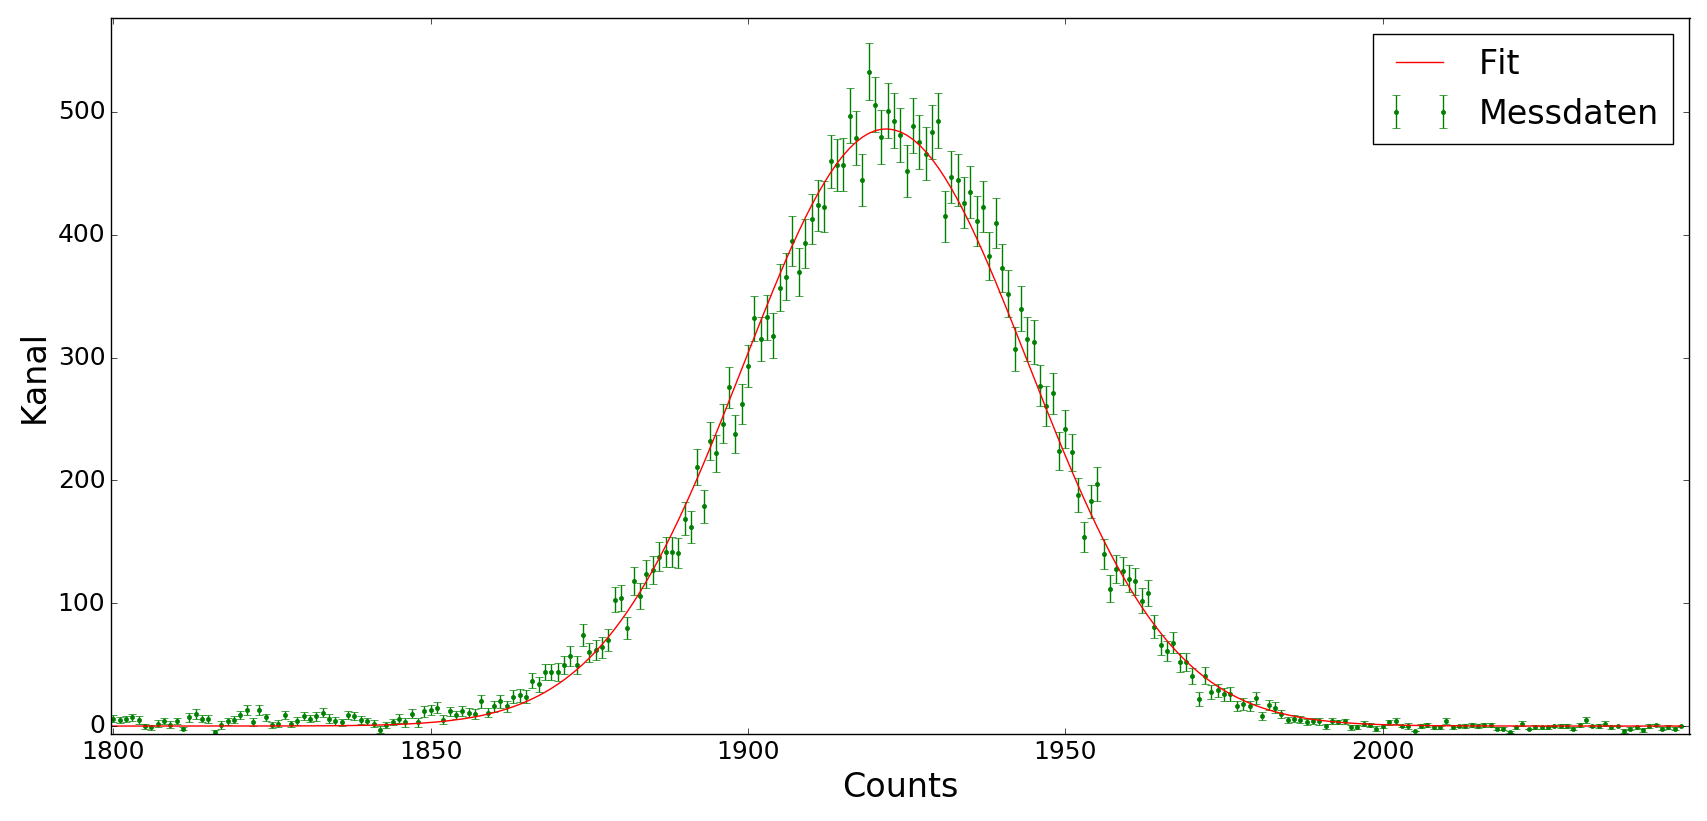
\includegraphics[scale = 0.39]{absrop_fit_blei_3.png}
\caption{Fit des Peaks mit 5,03cm Blei. Die Fitparameter sind in Tabelle \ref{tab:absorp_fit_3} eingetragen.}
\label{fig:absorp_fit_3}
\end{figure}

\begin{table}[H]
\centering
\caption{Fitparameter des Peaks mit 5,03cm Blei. Das $\chi^2_{red}$ ergab sich mit 1,71}
\label{tab:absorp_fit_3}
\begin{tabular}{|c|c|c|}
\hline Gau�peak & Parameter & Wert \\ 
\hline 1 & Amplitude & 27339(220) \\ 
\hline  & Center & 1921,7(2) \\ 
\hline  & Sigma & 22,4(1) \\ 
\hline 
\end{tabular} 
\end{table}



\begin{figure}[H]
\centering
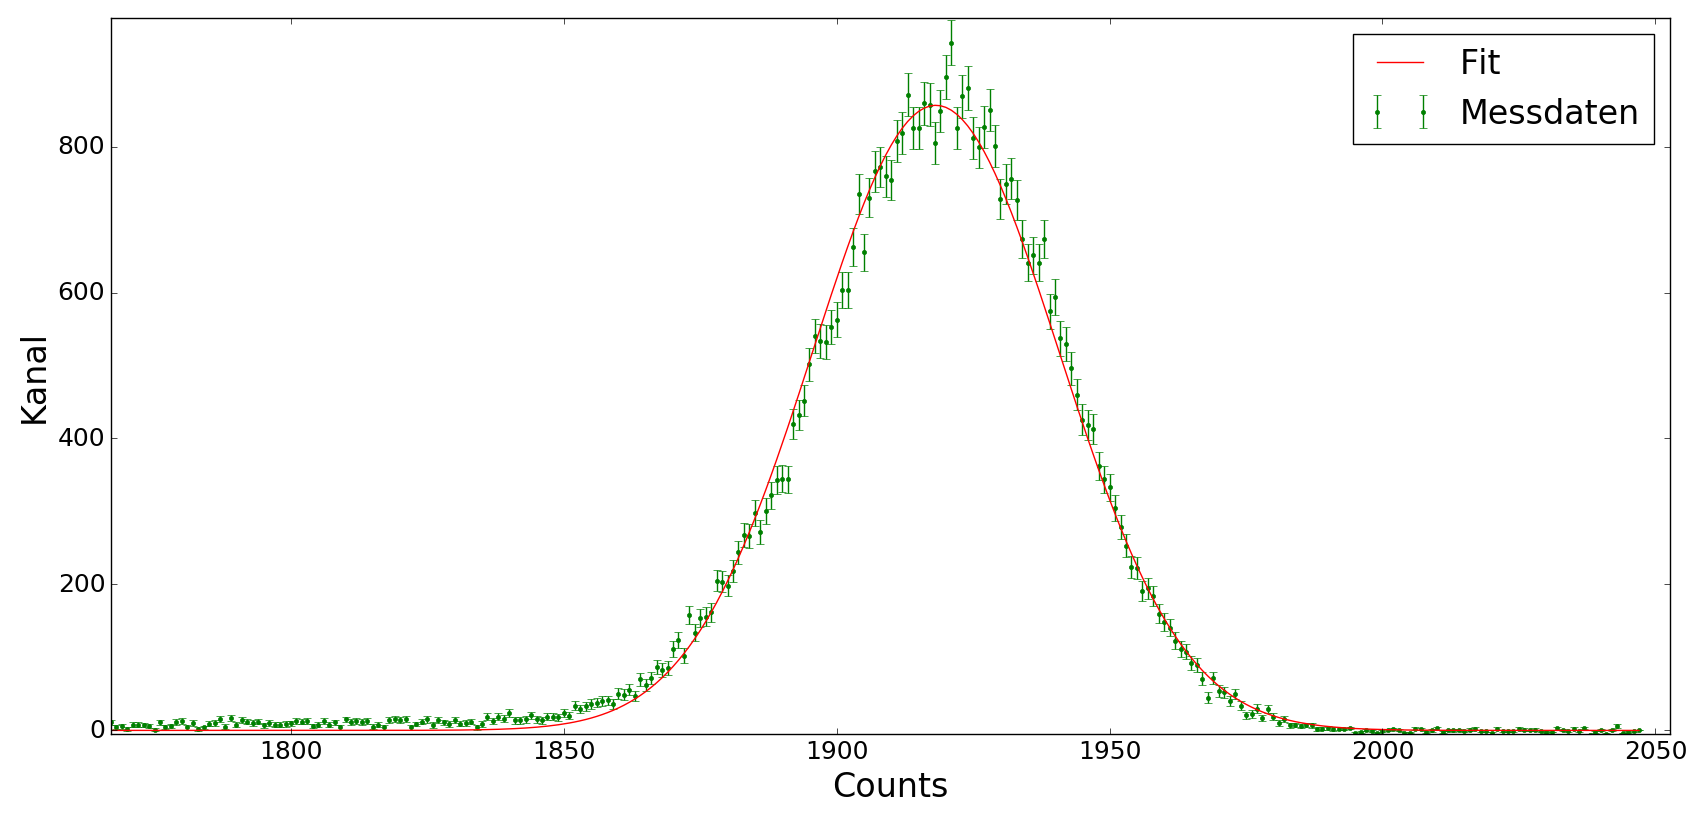
\includegraphics[scale = 0.39]{absrop_fit_blei_4.png}
\caption{Fit des Peaks mit 4,52cm Blei. Die Fitparameter sind in Tabelle \ref{tab:absorp_fit_4} eingetragen.}
\label{fig:absorp_fit_4}
\end{figure}

\begin{table}[H]
\centering
\caption{Fitparameter des Peaks mit 4,52cm Blei. Das $\chi^2_{red}$ ergab sich mit 2,52}
\label{tab:absorp_fit_4}
\begin{tabular}{|c|c|c|}
\hline Gau�peak & Parameter & Wert \\ 
\hline 1 & Amplitude & 48414(352) \\ 
\hline  & Center & 1918,2(2) \\ 
\hline  & Sigma & 22,6(1) \\ 
\hline 
\end{tabular} 
\end{table}



\begin{figure}[H]
\centering
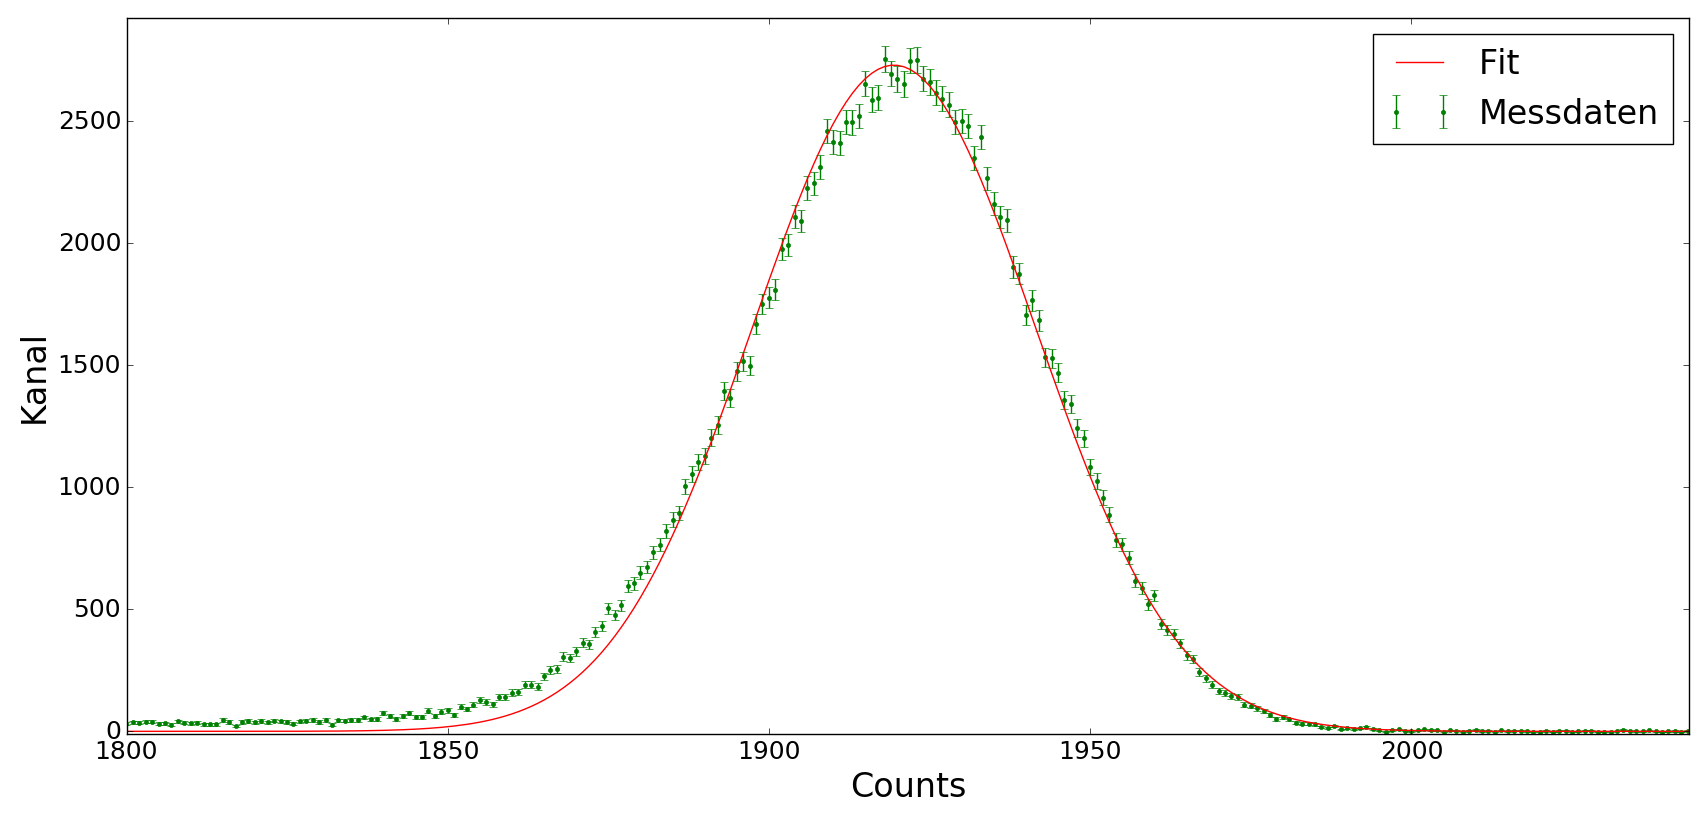
\includegraphics[scale = 0.39]{absrop_fit_blei_5.png}
\caption{Fit des Peaks mit 3,51cm Blei. Die Fitparameter sind in Tabelle \ref{tab:absorp_fit_5} eingetragen.}
\label{fig:absorp_fit_5}
\end{figure}

\begin{table}[H]
\centering
\caption{Fitparameter des Peaks mit 3,51cm Blei. Das $\chi^2_{red}$ ergab sich mit 2,72}
\label{tab:absorp_fit_5}
\begin{tabular}{|c|c|c|}
\hline Gau�peak & Parameter & Wert \\ 
\hline 1 & Amplitude & 150770(666) \\ 
\hline  & Center & 1919,5(1) \\ 
\hline  & Sigma & 22,02(9) \\ 
\hline 
\end{tabular} 
\end{table}





\begin{figure}[H]
\centering
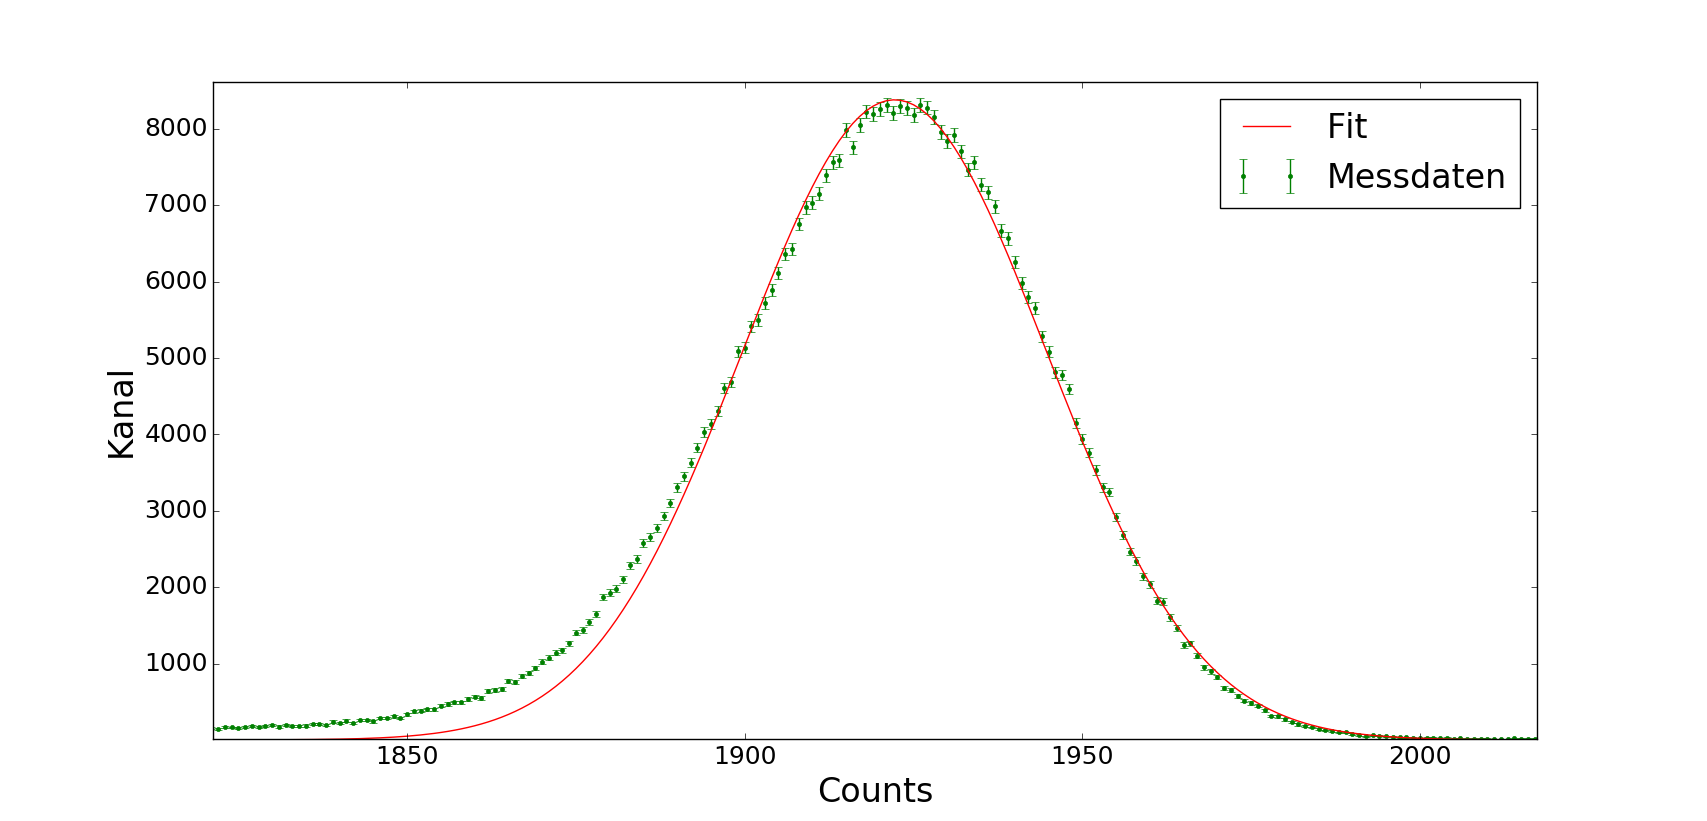
\includegraphics[scale = 0.39]{absrop_fit_blei_6.png}
\caption{Fit des Peaks mit 2,50cm Blei. Die Fitparameter sind in Tabelle \ref{tab:absorp_fit_6} eingetragen.}
\label{fig:absorp_fit_6}
\end{figure}

\begin{table}[H]
\centering
\caption{Fitparameter des Peaks mit 2,50cm Blei. Das $\chi^2_{red}$ ergab sich mit 4,18}
\label{tab:absorp_fit_6}
\begin{tabular}{|c|c|c|}
\hline Gau�peak & Parameter & Wert \\ 
\hline 1 & Amplitude & 473140(1630) \\ 
\hline  & Center & 1922,18(9) \\ 
\hline  & Sigma & 22,52(9) \\ 
\hline 
\end{tabular} 
\end{table}


\subsection{Aluminium}

\begin{figure}[H]
\centering
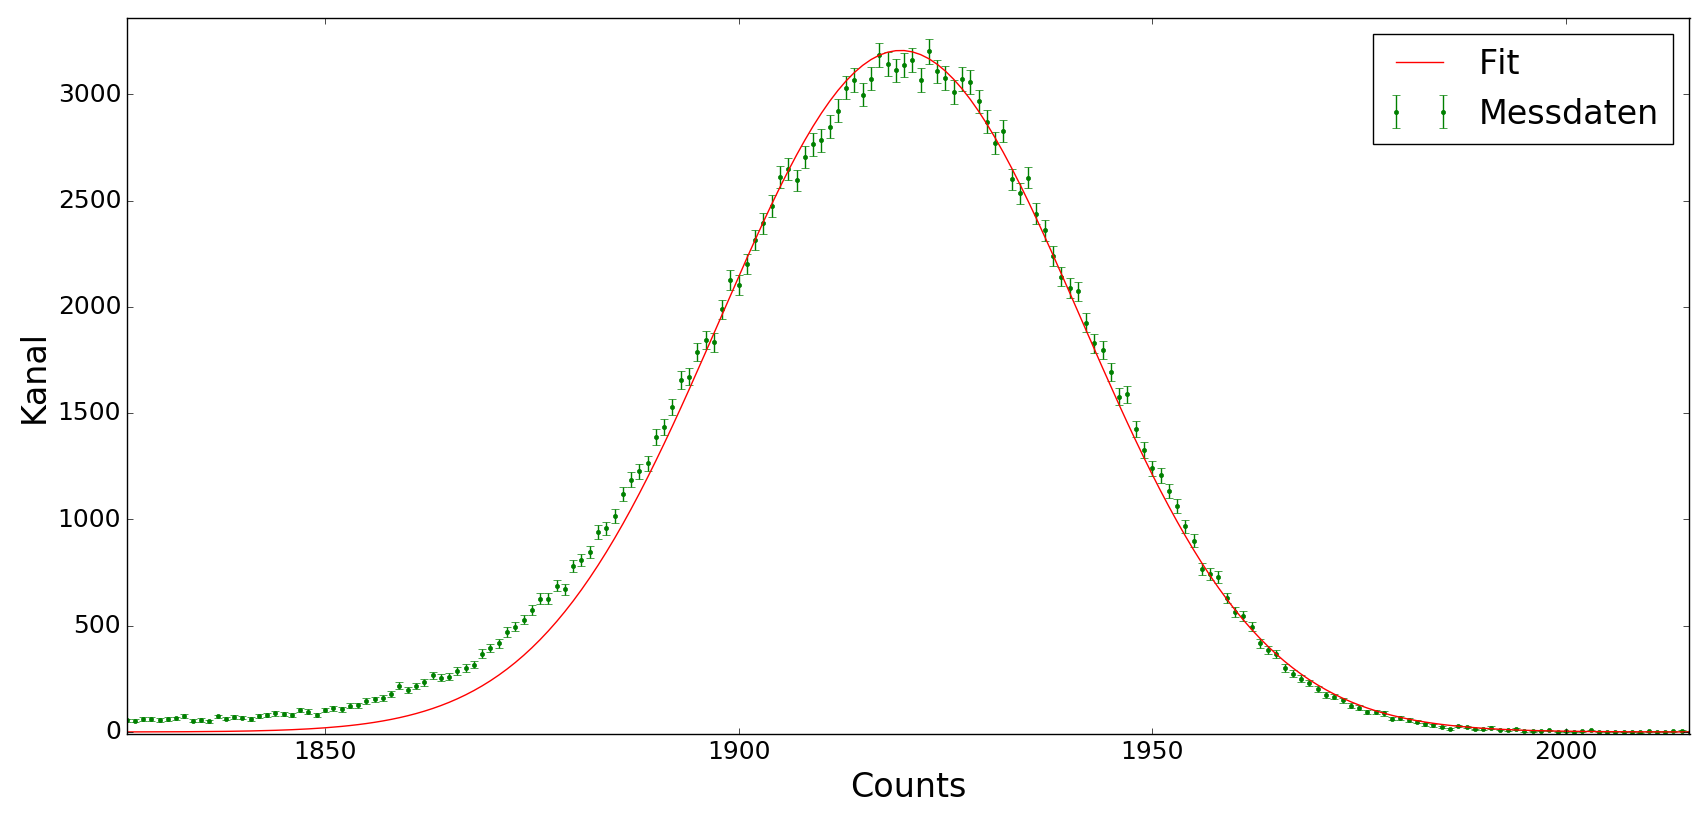
\includegraphics[scale = 0.39]{absrop_fit_alu_1.png}
\caption{Fit des Peaks mit 7,60cm Aluminium. Die Fitparameter sind in Tabelle \ref{tab:absorp_fit_alu_1} eingetragen.}
\label{fig:absorp_fit_alu_1}
\end{figure}

\begin{table}[H]
\centering
\caption{Fitparameter des Peaks mit 7,60cm Blei. Das $\chi^2_{red}$ ergab sich mit 2,18}
\label{tab:absorp_fit_alu_1}
\begin{tabular}{|c|c|c|}
\hline Gau�peak & Parameter & Wert \\ 
\hline 1 & Amplitude & 17520(705) \\ 
\hline  & Center & 1919,5(1) \\ 
\hline  & Sigma & 21,79(8) \\ 
\hline 
\end{tabular} 
\end{table}



\begin{figure}[H]
\centering
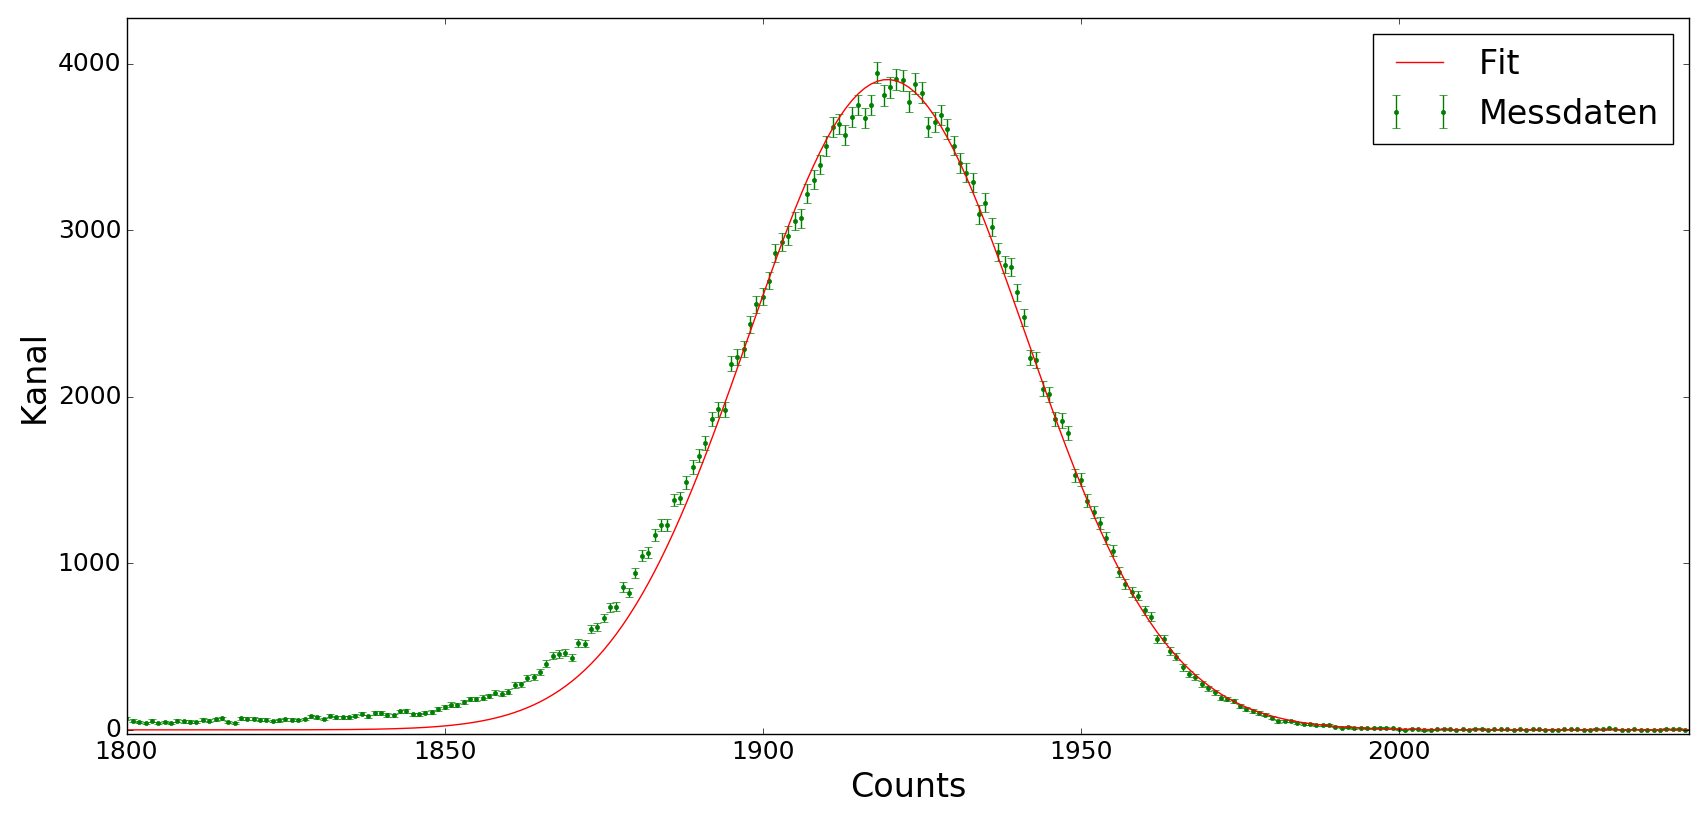
\includegraphics[scale = 0.39]{absrop_fit_alu_2.png}
\caption{Fit des Peaks mit 6,58cm Aluminium. Die Fitparameter sind in Tabelle \ref{tab:absorp_fit_alu_2} eingetragen.}
\label{fig:absorp_fit_alu_2}
\end{figure}

\begin{table}[H]
\centering
\caption{Fitparameter des Peaks mit 6,58cm Blei. Das $\chi^2_{red}$ ergab sich mit 1,77}
\label{tab:absorp_fit_alu_2}
\begin{tabular}{|c|c|c|}
\hline Gau�peak & Parameter & Wert \\ 
\hline 1 & Amplitude & 213170(696) \\ 
\hline  & Center & 1919,59(9) \\ 
\hline  & Sigma & 21,77(7) \\ 
\hline 
\end{tabular} 
\end{table}



\begin{figure}[H]
\centering
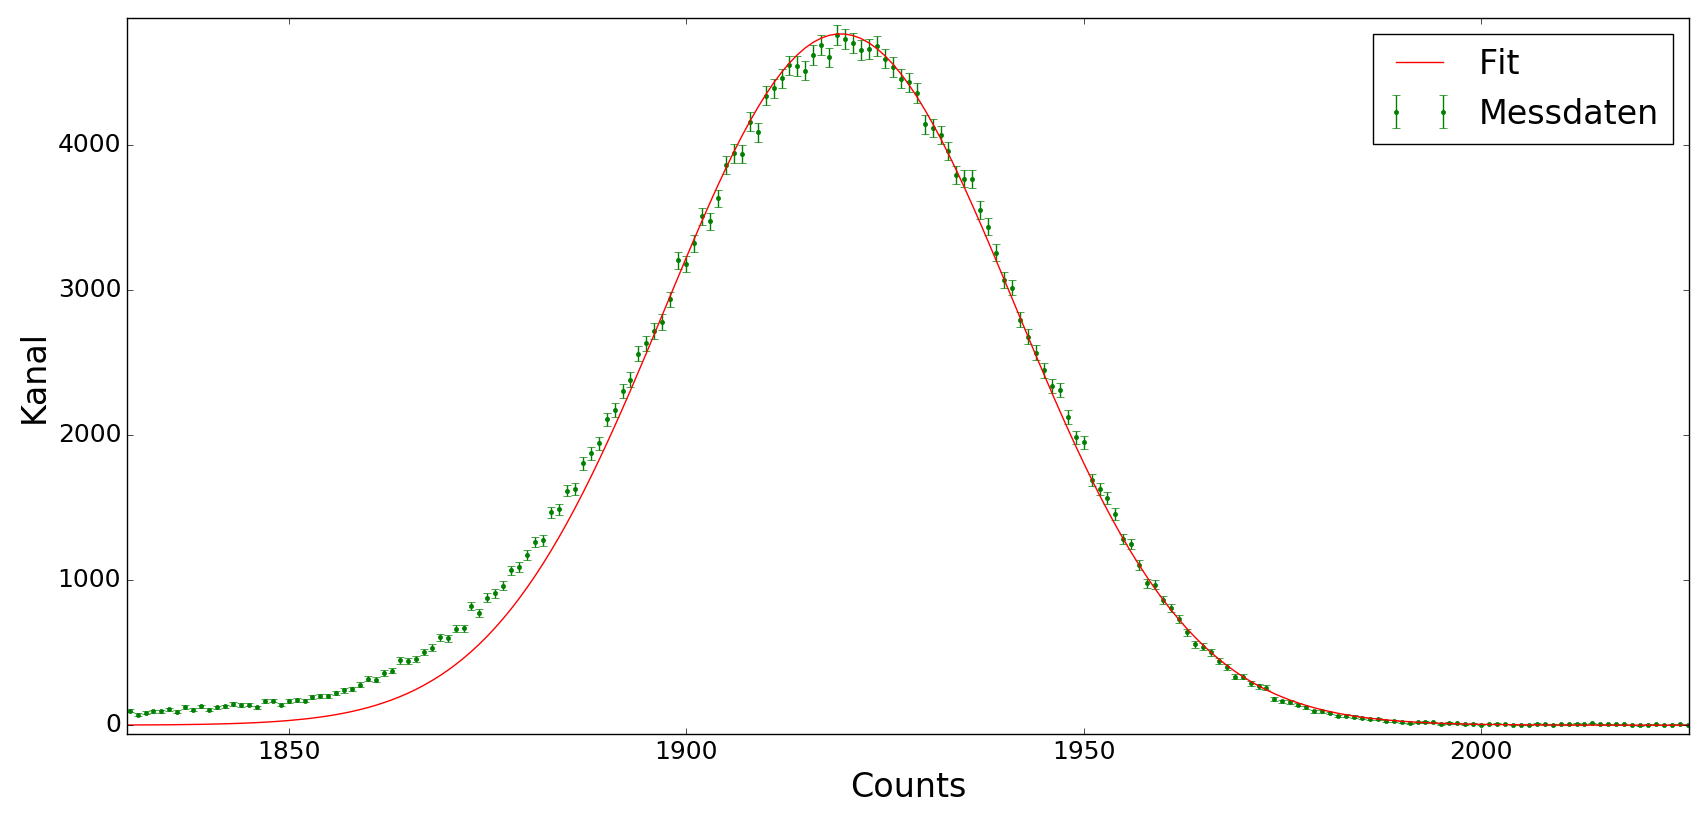
\includegraphics[scale = 0.39]{absrop_fit_alu_3.png}
\caption{Fit des Peaks mit 5,57cm Aluminium. Die Fitparameter sind in Tabelle \ref{tab:absorp_fit_alu_3} eingetragen.}
\label{fig:absorp_fit_alu_3}
\end{figure}

\begin{table}[H]
\centering
\caption{Fitparameter des Peaks mit 5,57cm Blei. Das $\chi^2_{red}$ ergab sich mit 1,91}
\label{tab:absorp_fit_alu_3}
\begin{tabular}{|c|c|c|}
\hline Gau�peak & Parameter & Wert \\ 
\hline 1 & Amplitude & 262160(815) \\ 
\hline  & Center & 1919,43(9) \\ 
\hline  & Sigma & 21,95(7) \\ 
\hline 
\end{tabular} 
\end{table}


\begin{figure}[H]
\centering
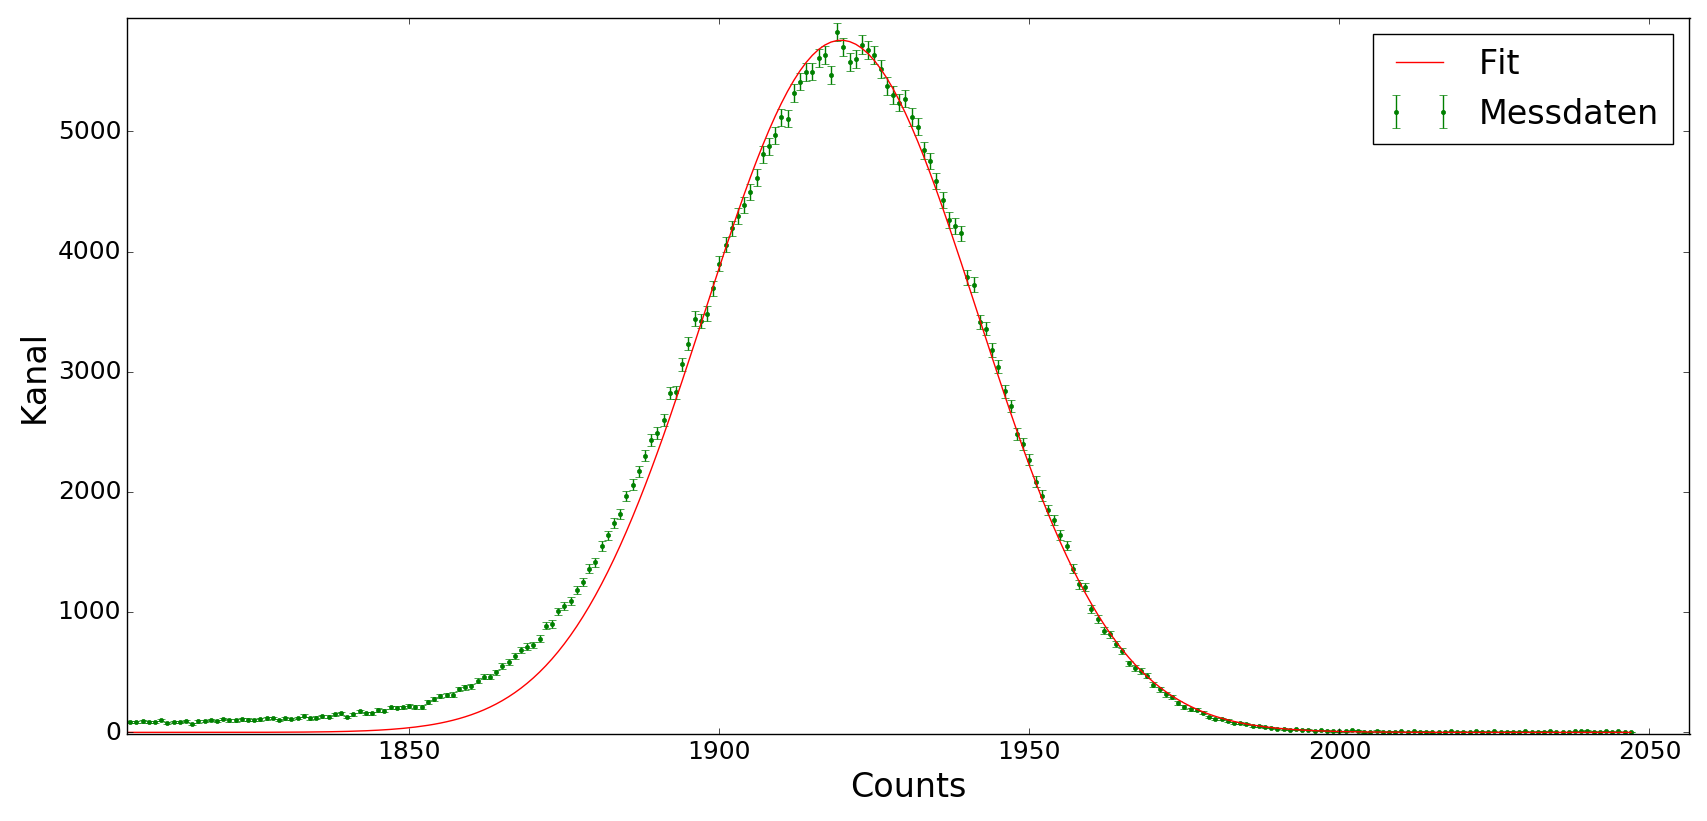
\includegraphics[scale = 0.39]{absrop_fit_alu_4.png}
\caption{Fit des Peaks mit 4,55cm Aluminium. Die Fitparameter sind in Tabelle \ref{tab:absorp_fit_alu_4} eingetragen.}
\label{fig:absorp_fit_alu_4}
\end{figure}

\begin{table}[H]
\centering
\caption{Fitparameter des Peaks mit 4,55cm Blei. Das $\chi^2_{red}$ ergab sich mit 2,32}
\label{tab:absorp_fit_alu_4}
\begin{tabular}{|c|c|c|}
\hline Gau�peak & Parameter & Wert \\ 
\hline 1 & Amplitude & 317600(982) \\ 
\hline  & Center & 1919,62(9) \\ 
\hline  & Sigma & 22,00(7) \\ 
\hline 
\end{tabular} 
\end{table}



\begin{figure}[H]
\centering
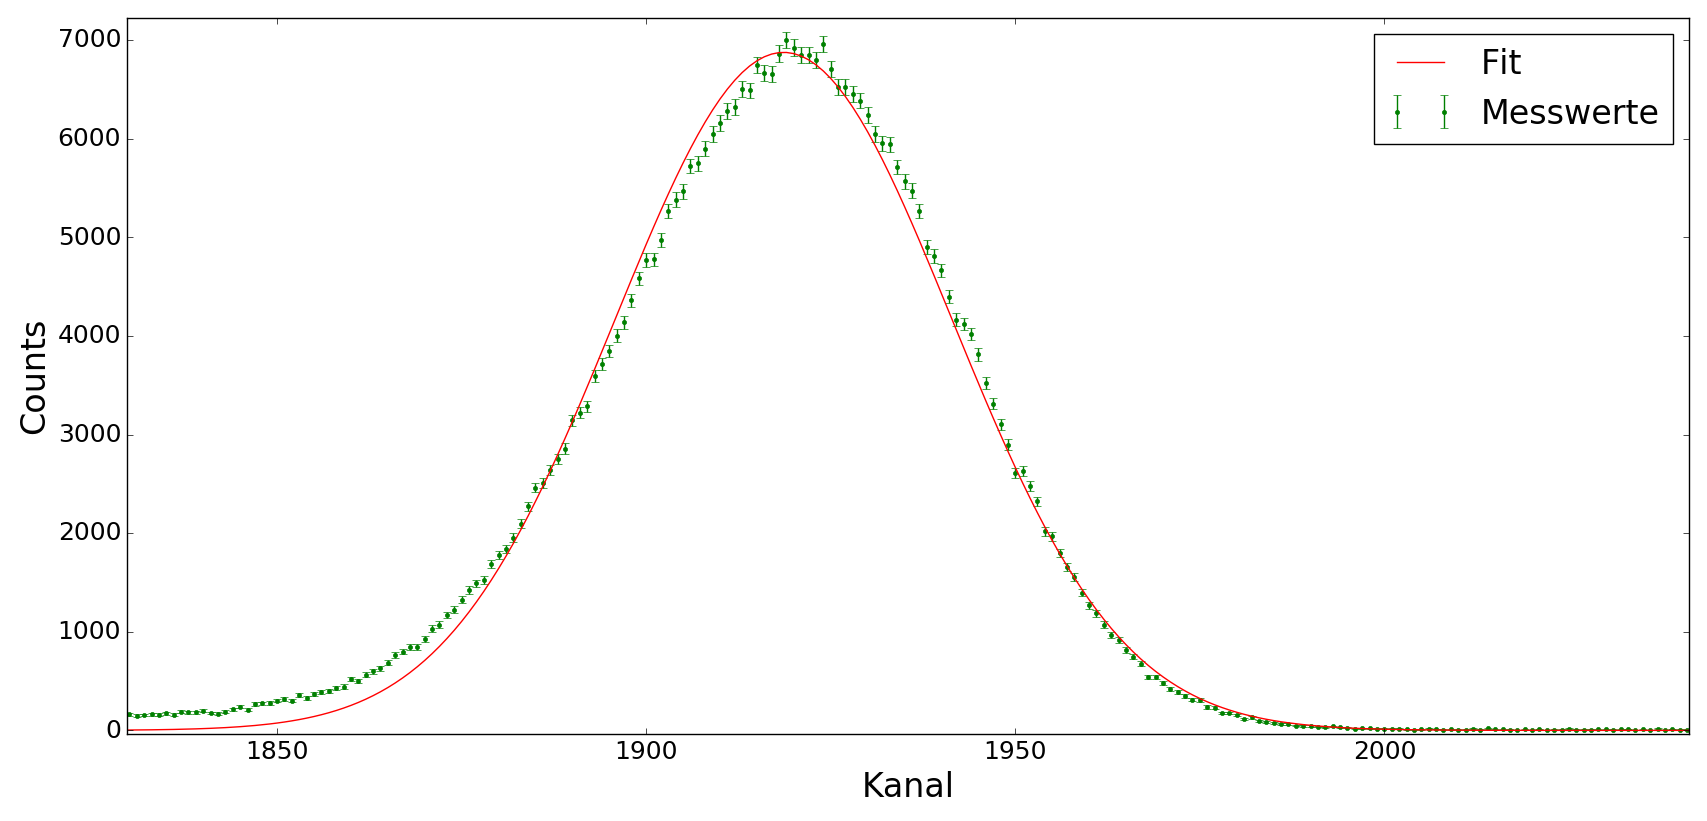
\includegraphics[scale = 0.39]{absrop_fit_alu_5.png}
\caption{Fit des Peaks mit 3,54cm Aluminium. Die Fitparameter sind in Tabelle \ref{tab:absorp_fit_alu_5} eingetragen.}
\label{fig:absorp_fit_alu_5}
\end{figure}

\begin{table}[H]
\centering
\caption{Fitparameter des Peaks mit 3,54cm Blei. Das $\chi^2_{red}$ ergab sich mit 8,72}
\label{tab:absorp_fit_alu_5}
\begin{tabular}{|c|c|c|}
\hline Gau�peak & Parameter & Wert \\ 
\hline 1 & Amplitude & 393100(1880) \\ 
\hline  & Center & 1918,6(1) \\ 
\hline  & Sigma & 22,81(9) \\ 
\hline 
\end{tabular} 
\end{table}
\section{Wirkungsquerschnitt}
In diesem Abschnitt werden die Plots und Fits der Energiemessungen f�r die Winkel von \SI{20}{\degree} bis \SI{80}{\degree} mit den zugeh�rigen Fitparametern dargestellt.
\label{Anh:WQ}
\begin{figure}[H]
\centering
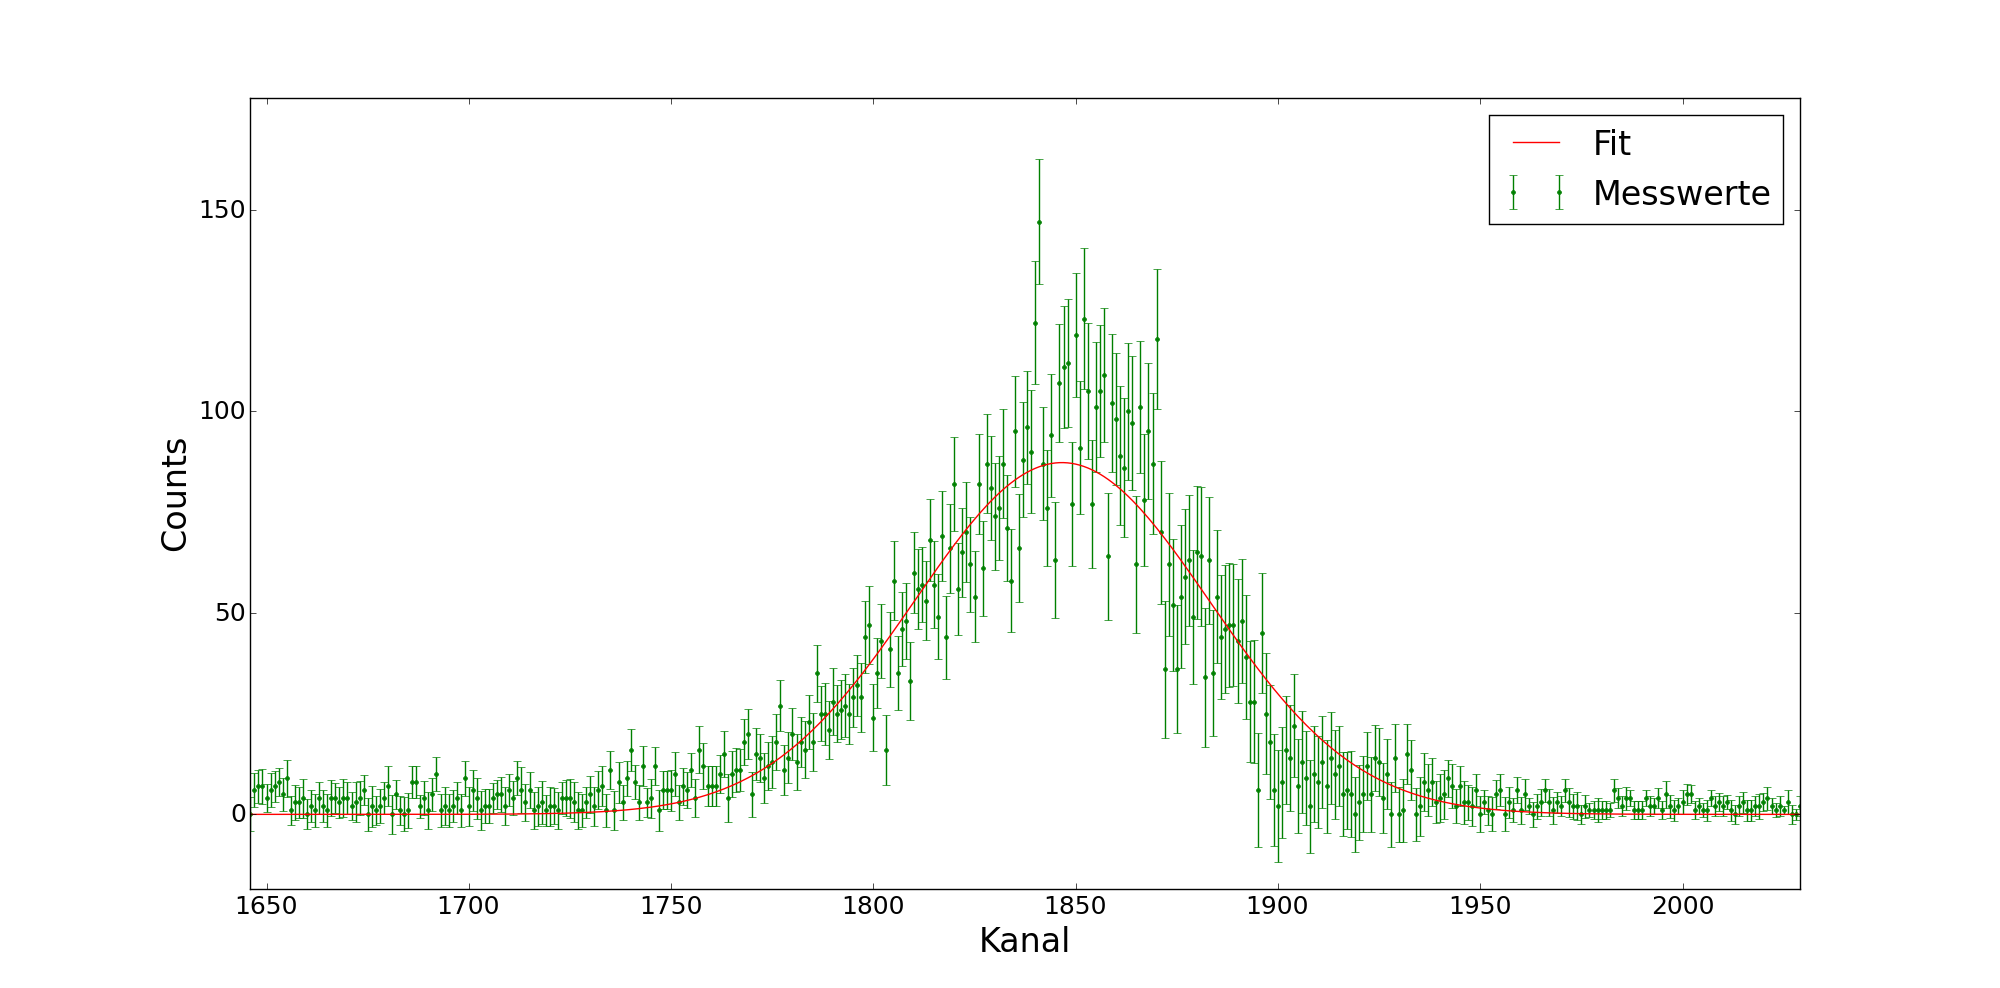
\includegraphics[scale = 0.34]{Wirkungsquerschnitt_20_Grad_Fit.png}
\caption{Die Fitparameter sind in Tabelle \ref{tab:20_Grad_WQ} eingetragen.}
\label{fig:Wirkungsquerschnitt_20}
\end{figure}

\begin{table}[H]
\centering
\caption{Fitparameter f�r die Energiemessung bei \SI{20}{\degree}. Das $\chi^2_{red}$ ergab sich mit 0,937}
\label{tab:20_Grad_WQ}
\begin{tabular}{|c|c|c|}
\hline Gau�peak & Parameter & Wert \\ 
\hline 1 & Amplitude & 7672(159) \\ 
\hline  & Center & 1843.2(97) \\ 
\hline  & Sigma & 34.9(6) \\ 
\hline 
\end{tabular} 
\end{table}

\begin{figure}[H]
\centering
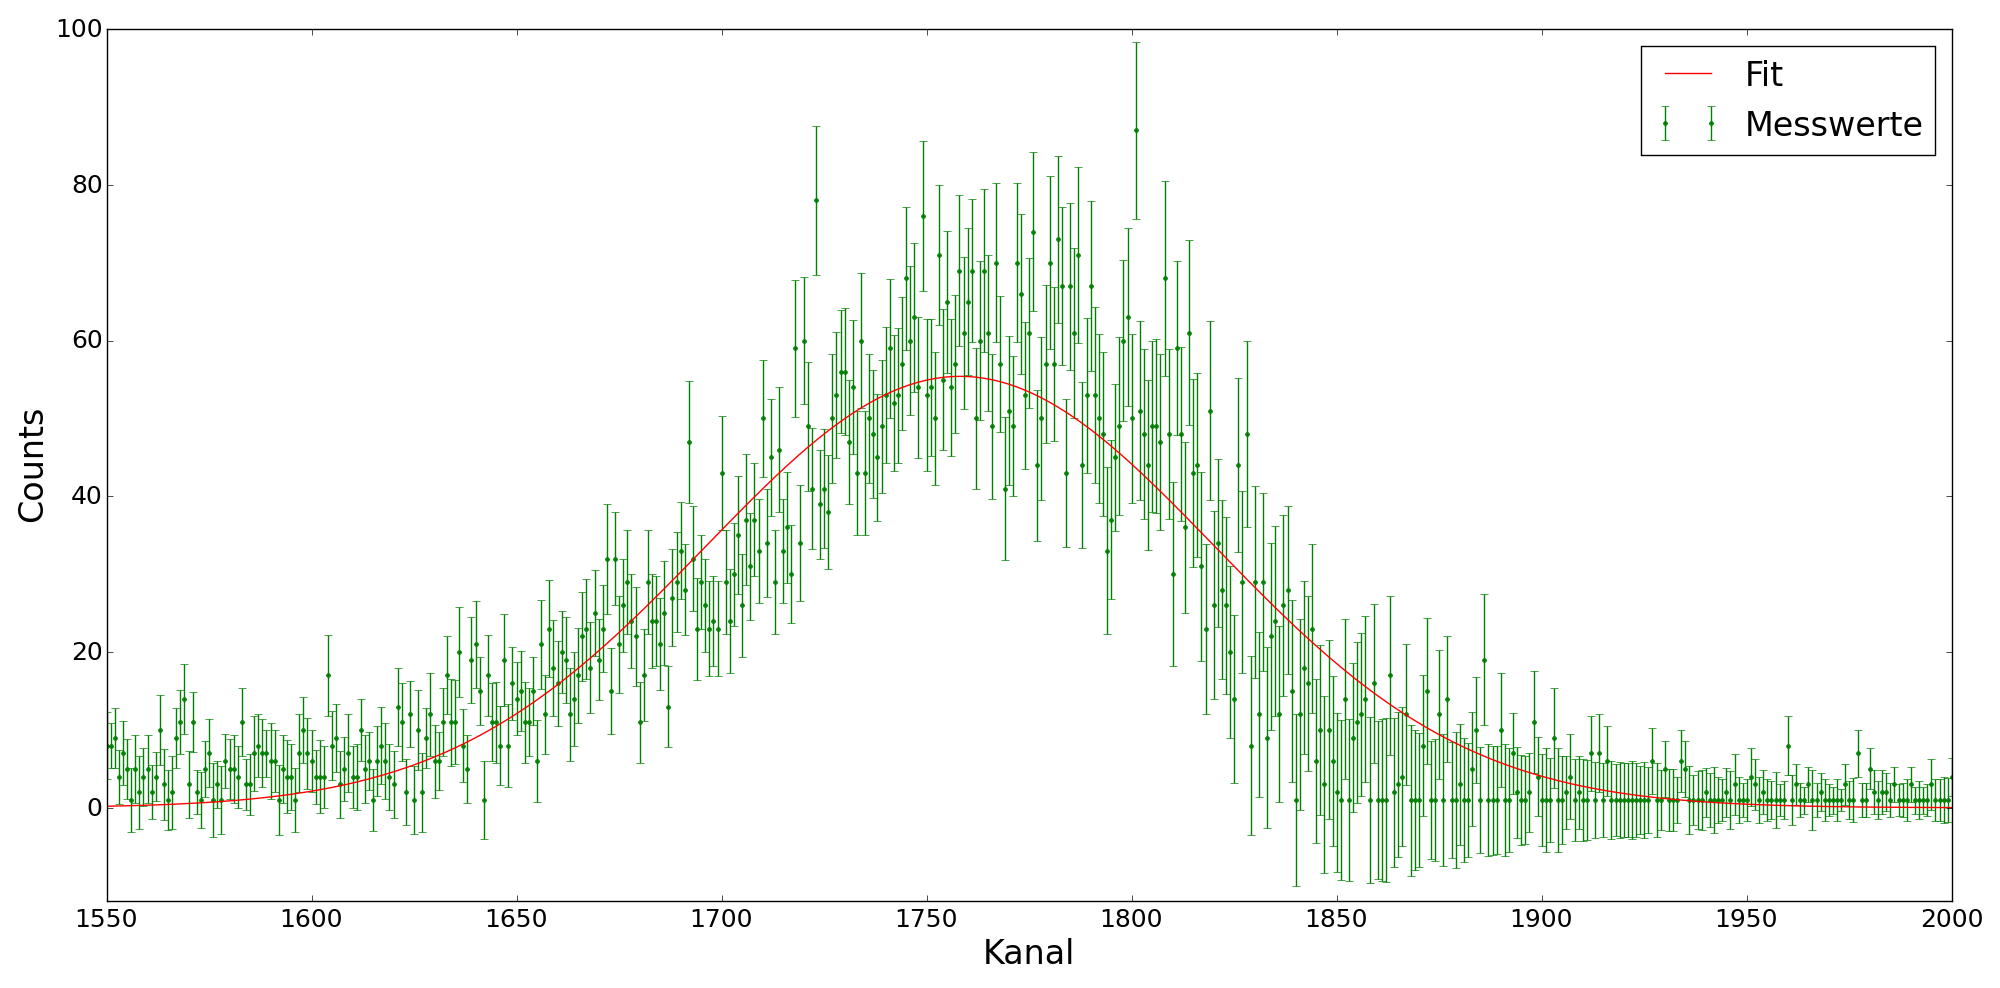
\includegraphics[scale = 0.34]{Wirkungsquerschnitt_30_Grad_Fit.png}
\caption{Die Fitparameter sind in Tabelle \ref{tab:30_Grad_WQ} eingetragen.}
\label{fig:Wirkungsquerschnitt_30}
\end{figure}

\begin{table}[H]
\centering
\caption{Fitparameter f�r die Energiemessung bei \SI{30}{\degree}. Das $\chi^2_{red}$ ergab sich mit 1.086}
\label{tab:30_Grad_WQ}
\begin{tabular}{|c|c|c|}
\hline Gau�peak & Parameter & Wert \\ 
\hline 1 & Amplitude & 8611(141) \\ 
\hline  & Center & 1758(1) \\ 
\hline  & Sigma & 62(1) \\ 
\hline 
\end{tabular} 
\end{table}

\begin{figure}[H]
\centering
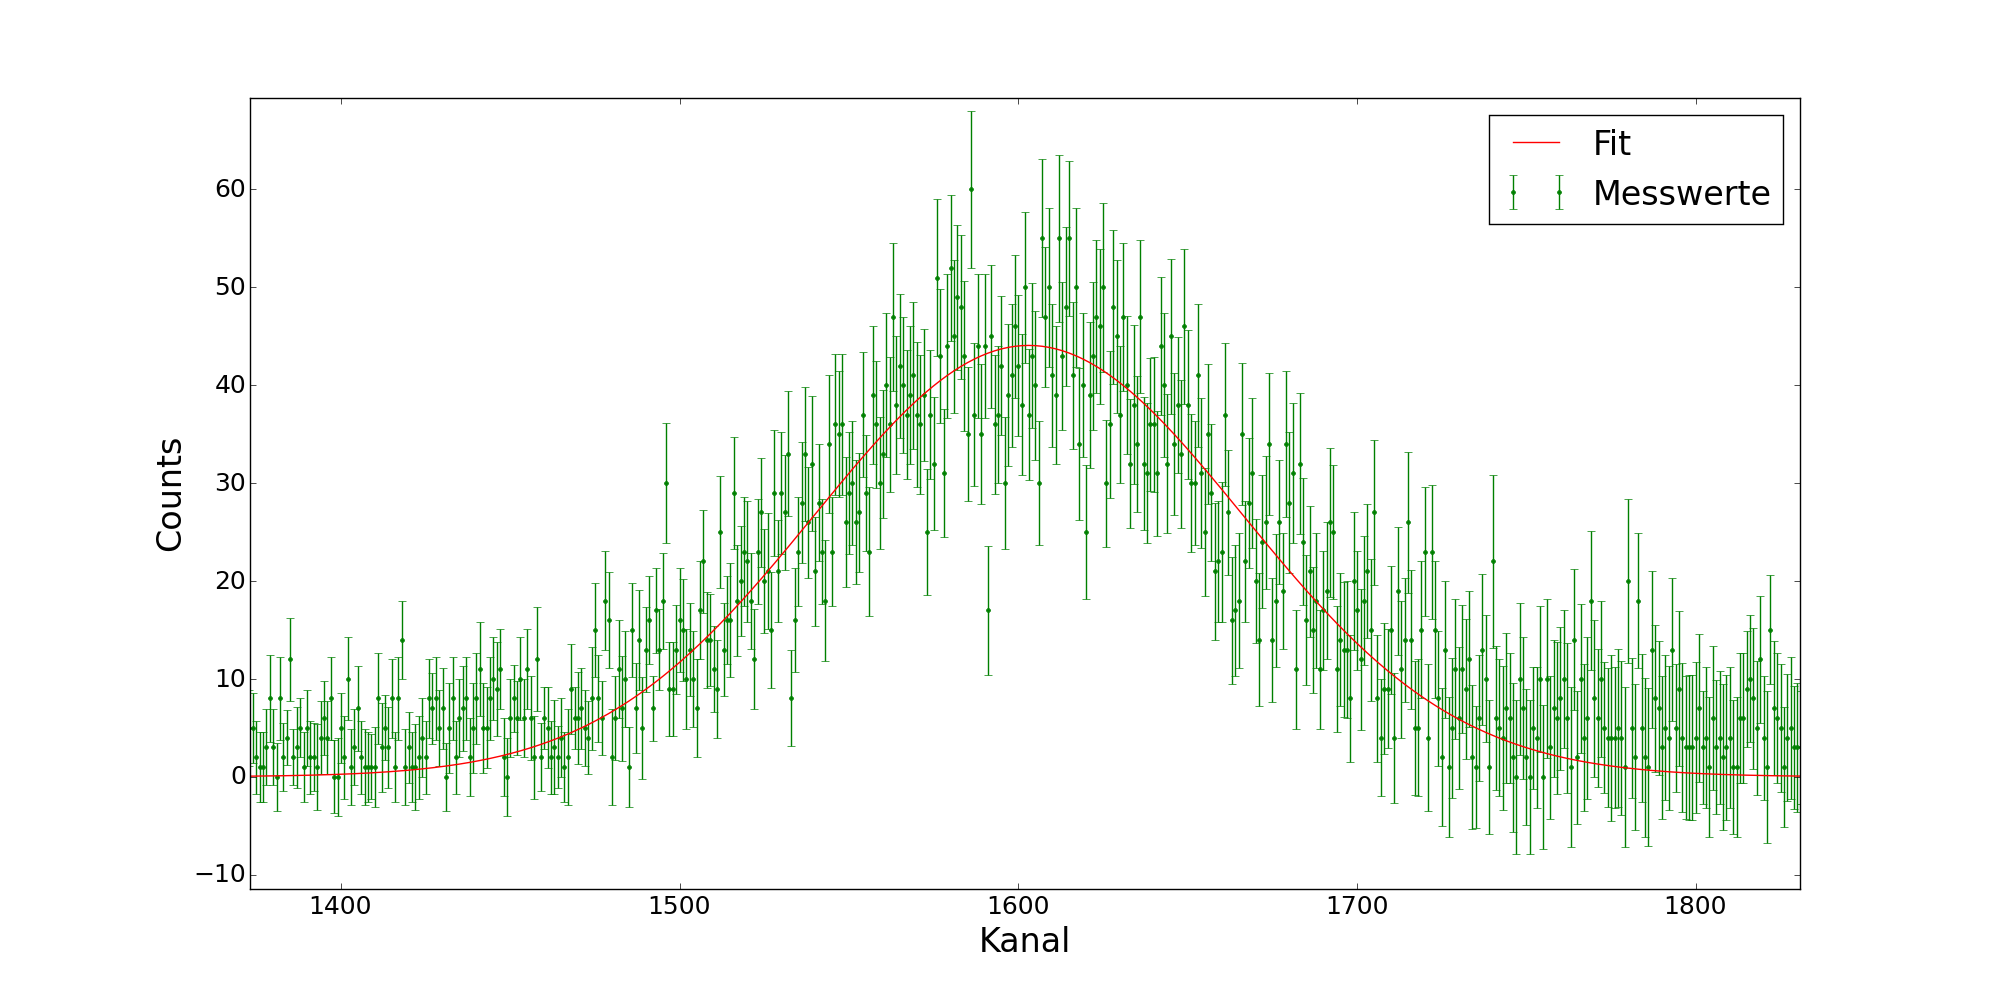
\includegraphics[scale = 0.34]{Wirkungsquerschnitt_40_Grad_Fit.png}
\caption{Die Fitparameter sind in Tabelle \ref{tab:40_Grad_WQ} eingetragen.}
\label{fig:Wirkungsquerschnitt_40}
\end{figure}

\begin{table}[H]
\centering
\caption{Fitparameter f�r die Energiemessung bei \SI{40}{\degree}. Das $\chi^2_{red}$ ergab sich mit 0.994}
\label{tab:40_Grad_WQ}
\begin{tabular}{|c|c|c|}
\hline Gau�peak & Parameter & Wert \\ 
\hline 1 & Amplitude & 6870(103) \\ 
\hline  & Center & 1602(1) \\ 
\hline  & Sigma & 63(1) \\ 
\hline 
\end{tabular} 
\end{table}

\begin{figure}[H]
\centering
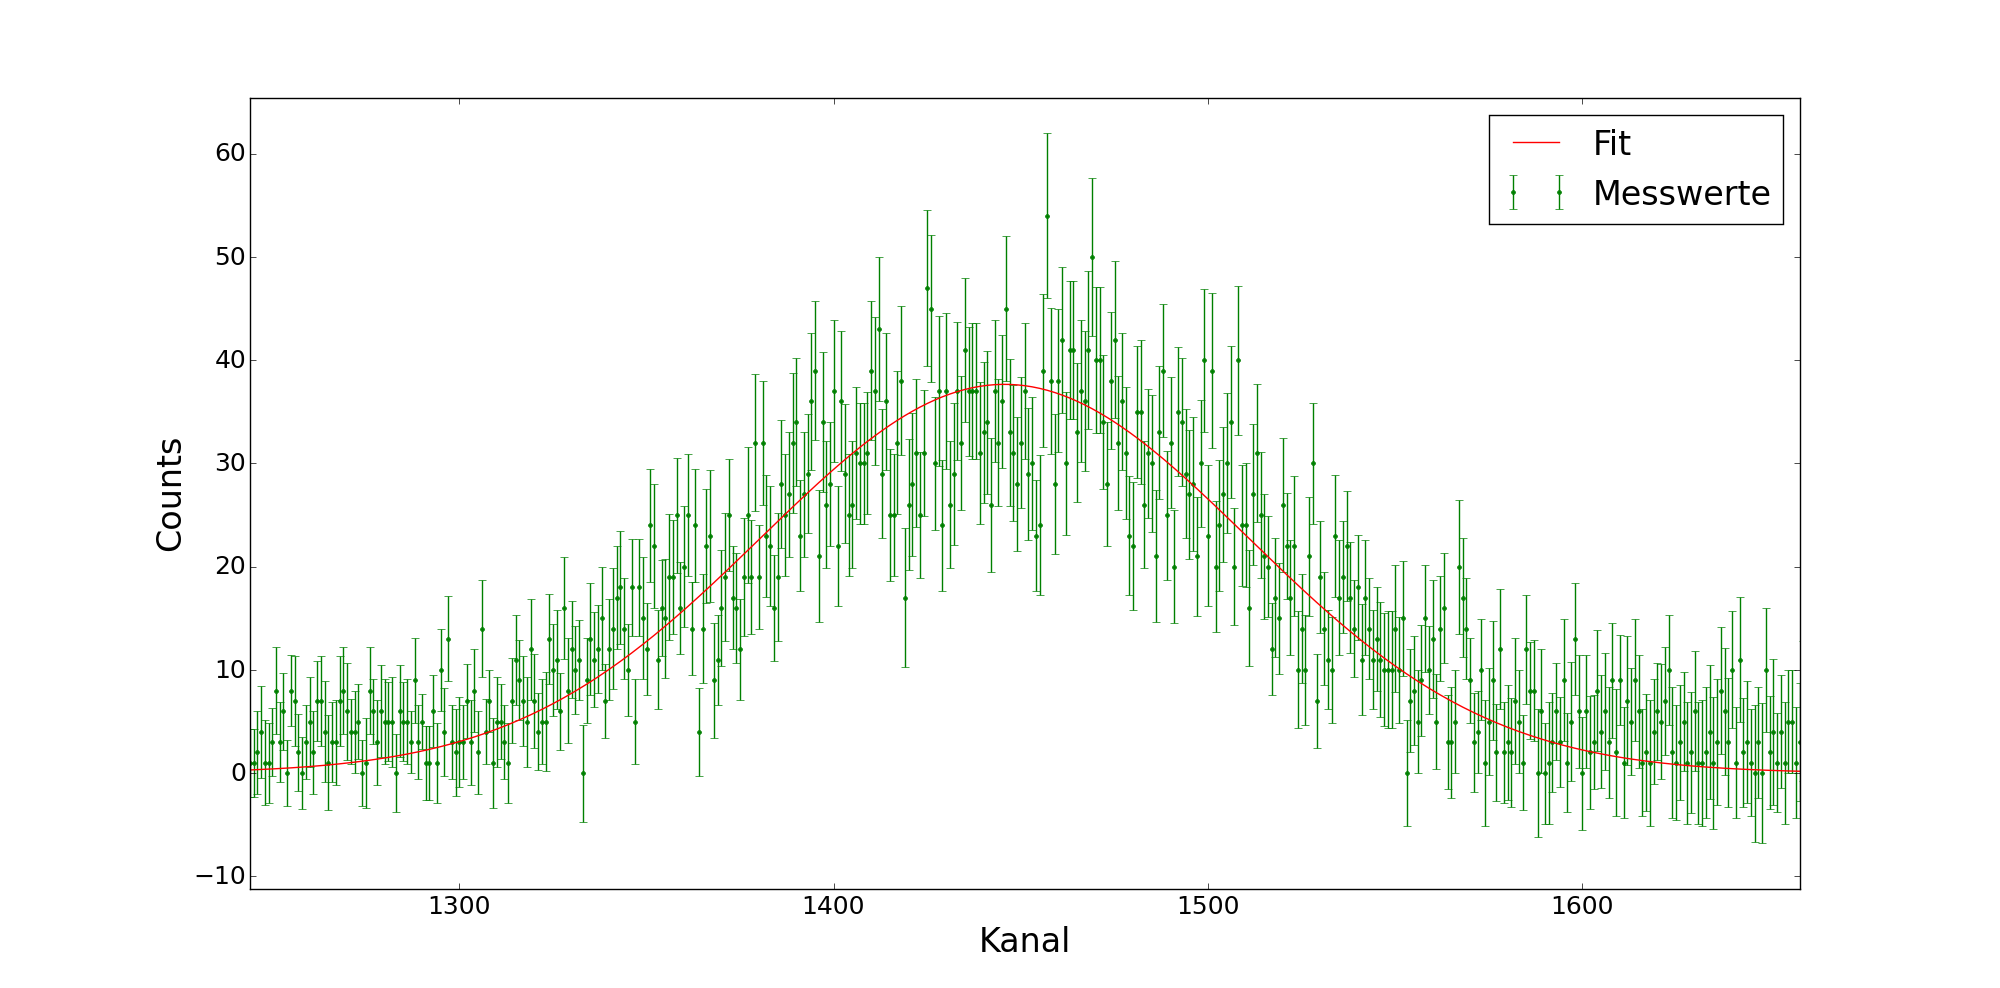
\includegraphics[scale = 0.34]{Wirkungsquerschnitt_50_Grad_Fit.png}
\caption{Die Fitparameter sind in Tabelle \ref{tab:50_Grad_WQ} eingetragen.}
\label{fig:Wirkungsquerschnitt_50}
\end{figure}

\begin{table}[H]
\centering
\caption{Fitparameter f�r die Energiemessung bei \SI{50}{\degree}. Das $\chi^2_{red}$ ergab sich mit 0.971}
\label{tab:50_Grad_WQ}
\begin{tabular}{|c|c|c|}
\hline Gau�peak & Parameter & Wert \\ 
\hline 1 & Amplitude & 5897(93) \\ 
\hline  & Center & 1445(1) \\ 
\hline  & Sigma & 63(1) \\ 
\hline 
\end{tabular} 
\end{table}

\begin{figure}[H]
\centering
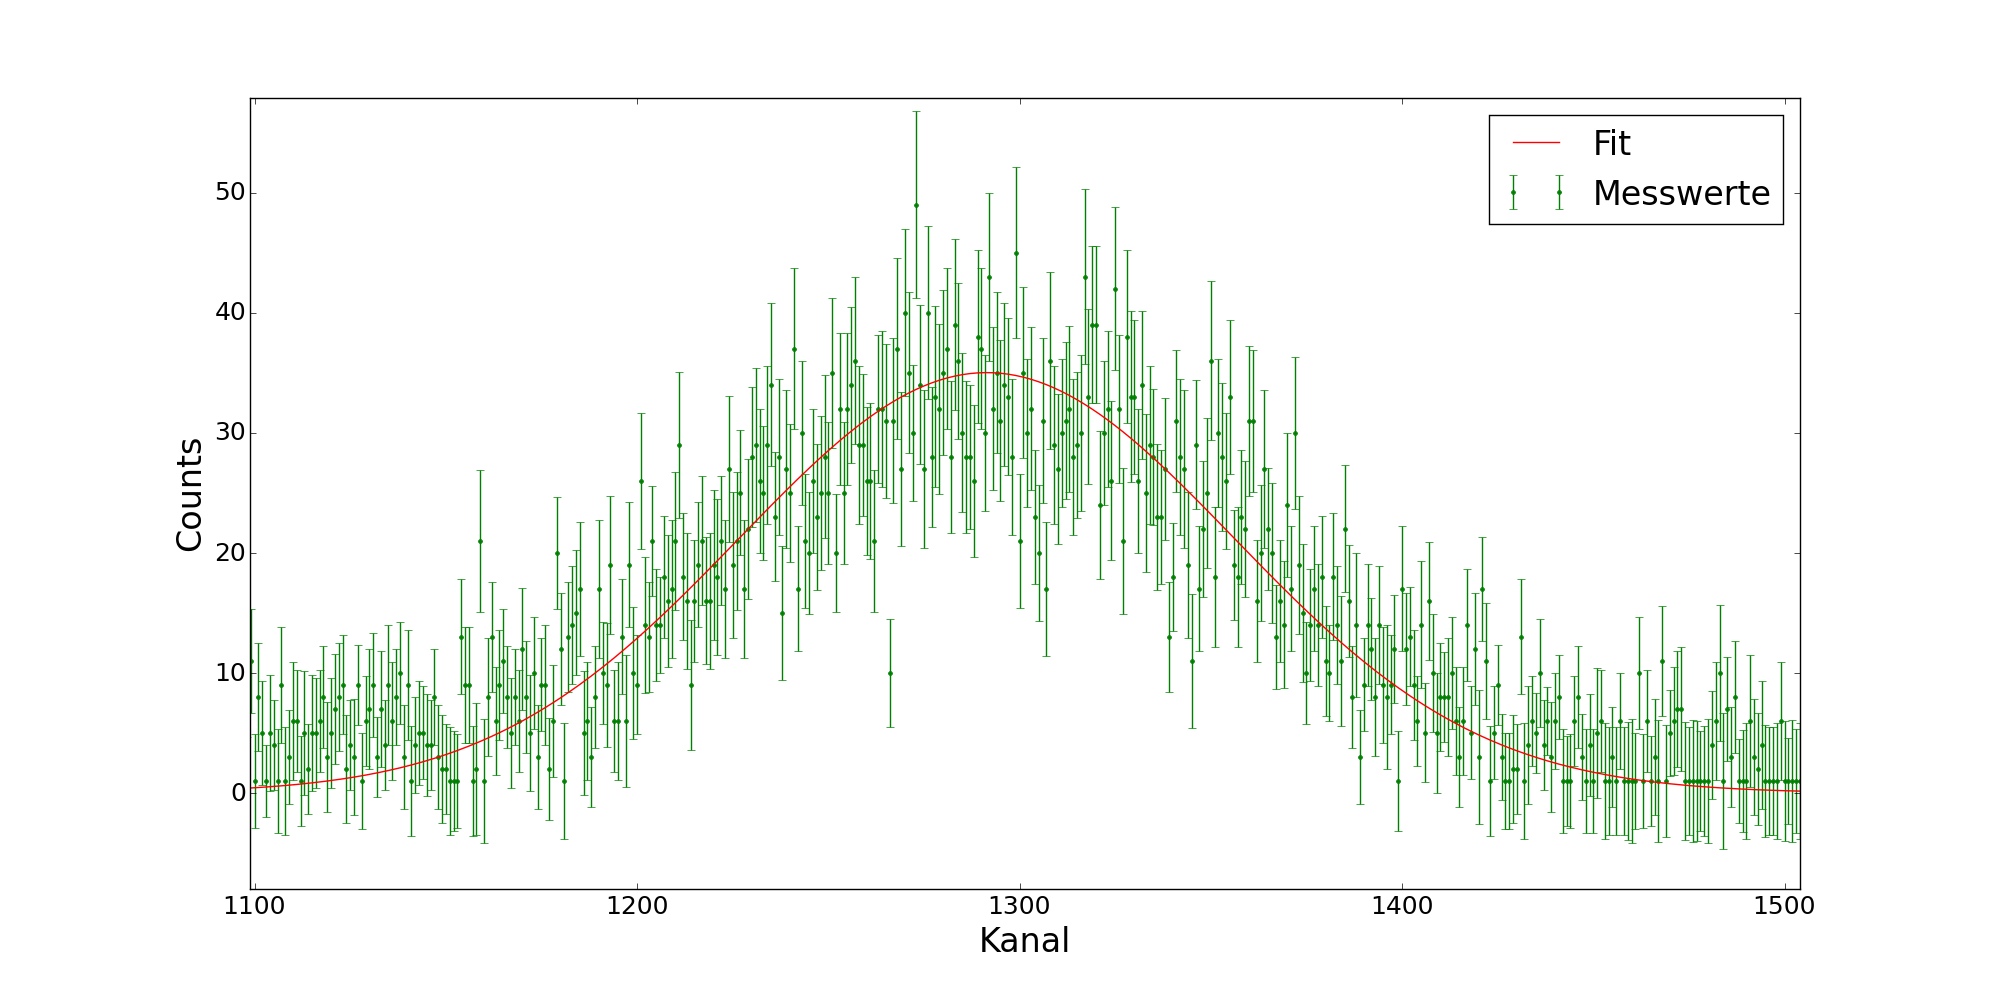
\includegraphics[scale = 0.34]{Wirkungsquerschnitt_60_Grad_Fit.png}
\caption{Die Fitparameter sind in Tabelle \ref{tab:60_Grad_WQ} eingetragen.}
\label{fig:Wirkungsquerschnitt_60}
\end{figure}

\begin{table}[H]
\centering
\caption{Fitparameter f�r die Energiemessung bei \SI{60}{\degree}. Das $\chi^2_{red}$ ergab sich mit 1.062}
\label{tab:60_Grad_WQ}
\begin{tabular}{|c|c|c|}
\hline Gau�peak & Parameter & Wert \\ 
\hline 1 & Amplitude & 5432(93) \\ 
\hline  & Center & 1291(1) \\ 
\hline  & Sigma & 63(1) \\ 
\hline 
\end{tabular} 
\end{table}

\begin{figure}[H]
\centering
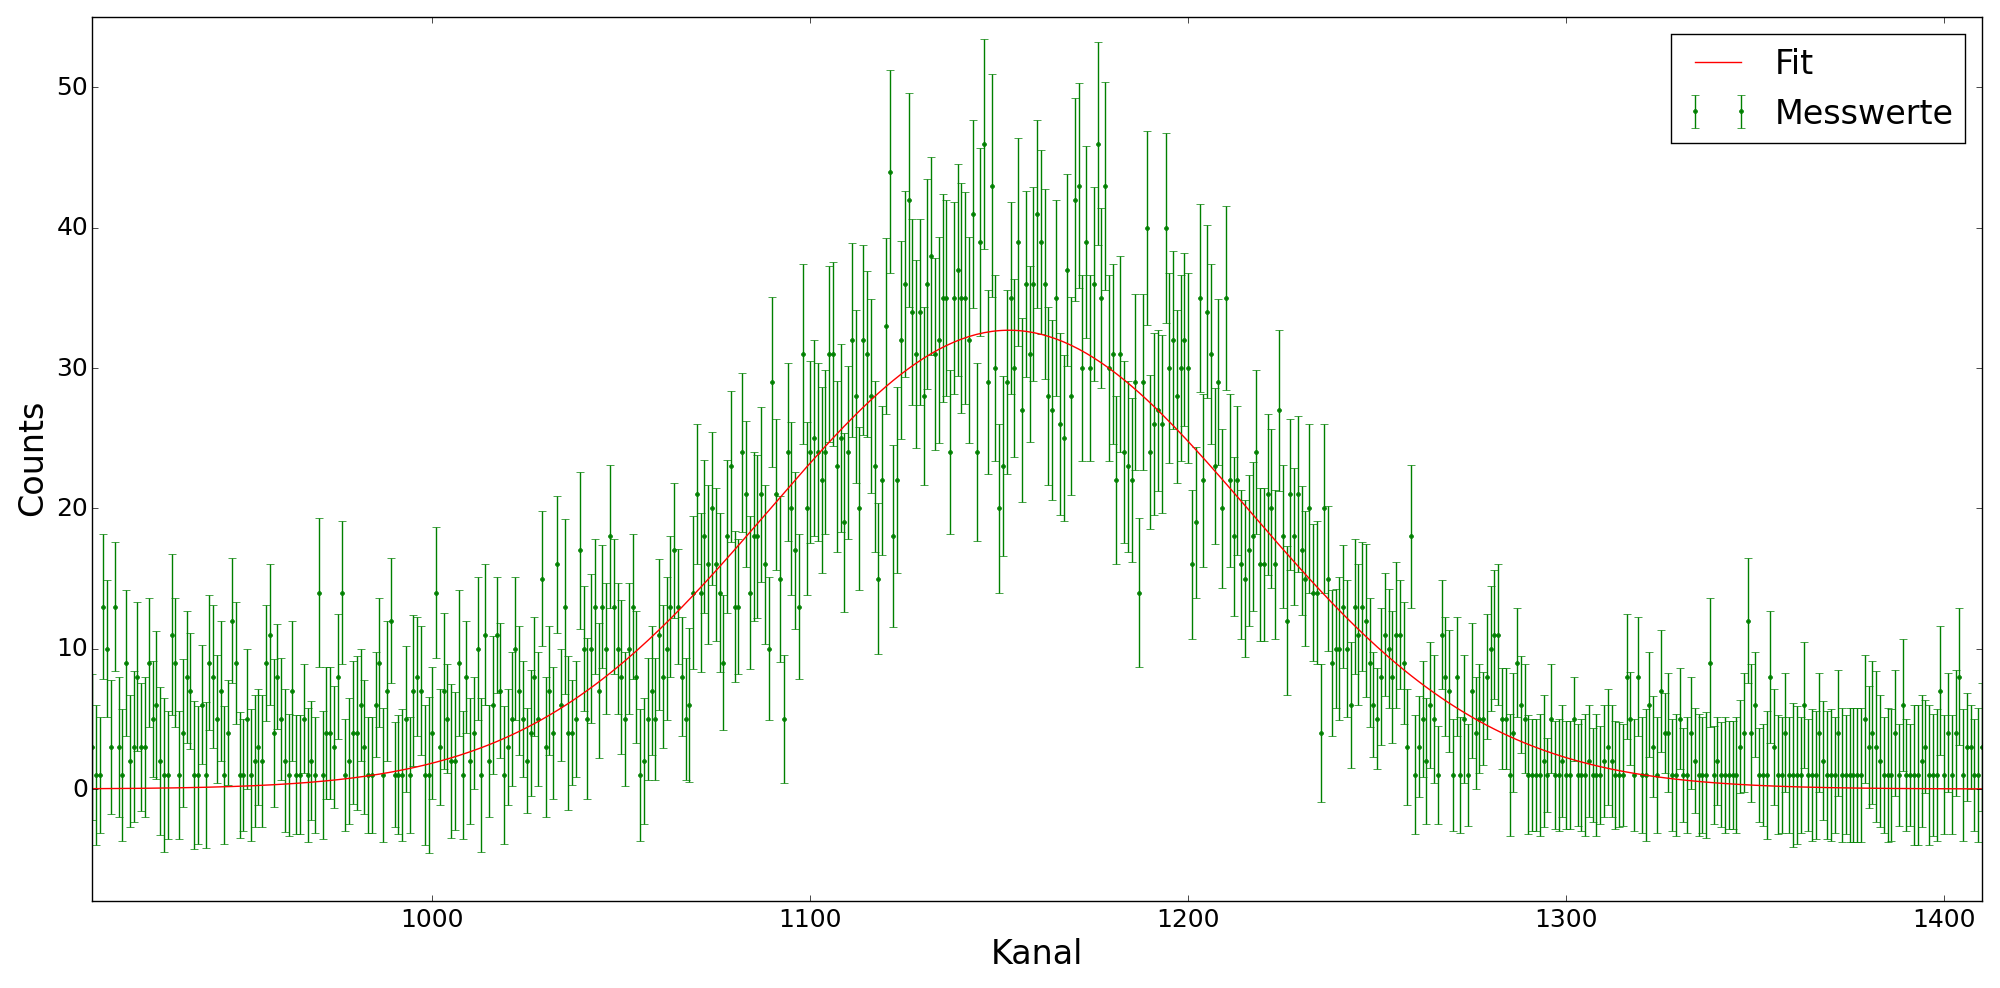
\includegraphics[scale = 0.34]{Wirkungsquerschnitt_70_Grad_Fit.png}
\caption{Die Fitparameter sind in Tabelle \ref{tab:70_Grad_WQ} eingetragen.}
\label{fig:Wirkungsquerschnitt_70}
\end{figure}

\begin{table}[H]
\centering
\caption{Fitparameter f�r die Energiemessung bei \SI{70}{\degree}. Das $\chi^2_{red}$ ergab sich mit 0.934}
\label{tab:70_Grad_WQ}
\begin{tabular}{|c|c|c|}
\hline Gau�peak & Parameter & Wert \\ 
\hline 1 & Amplitude & 5214(94) \\ 
\hline  & Center & 1153(1) \\ 
\hline  & Sigma & 63.6(6) \\ 
\hline 
\end{tabular} 
\end{table}

\begin{figure}[H]
\centering
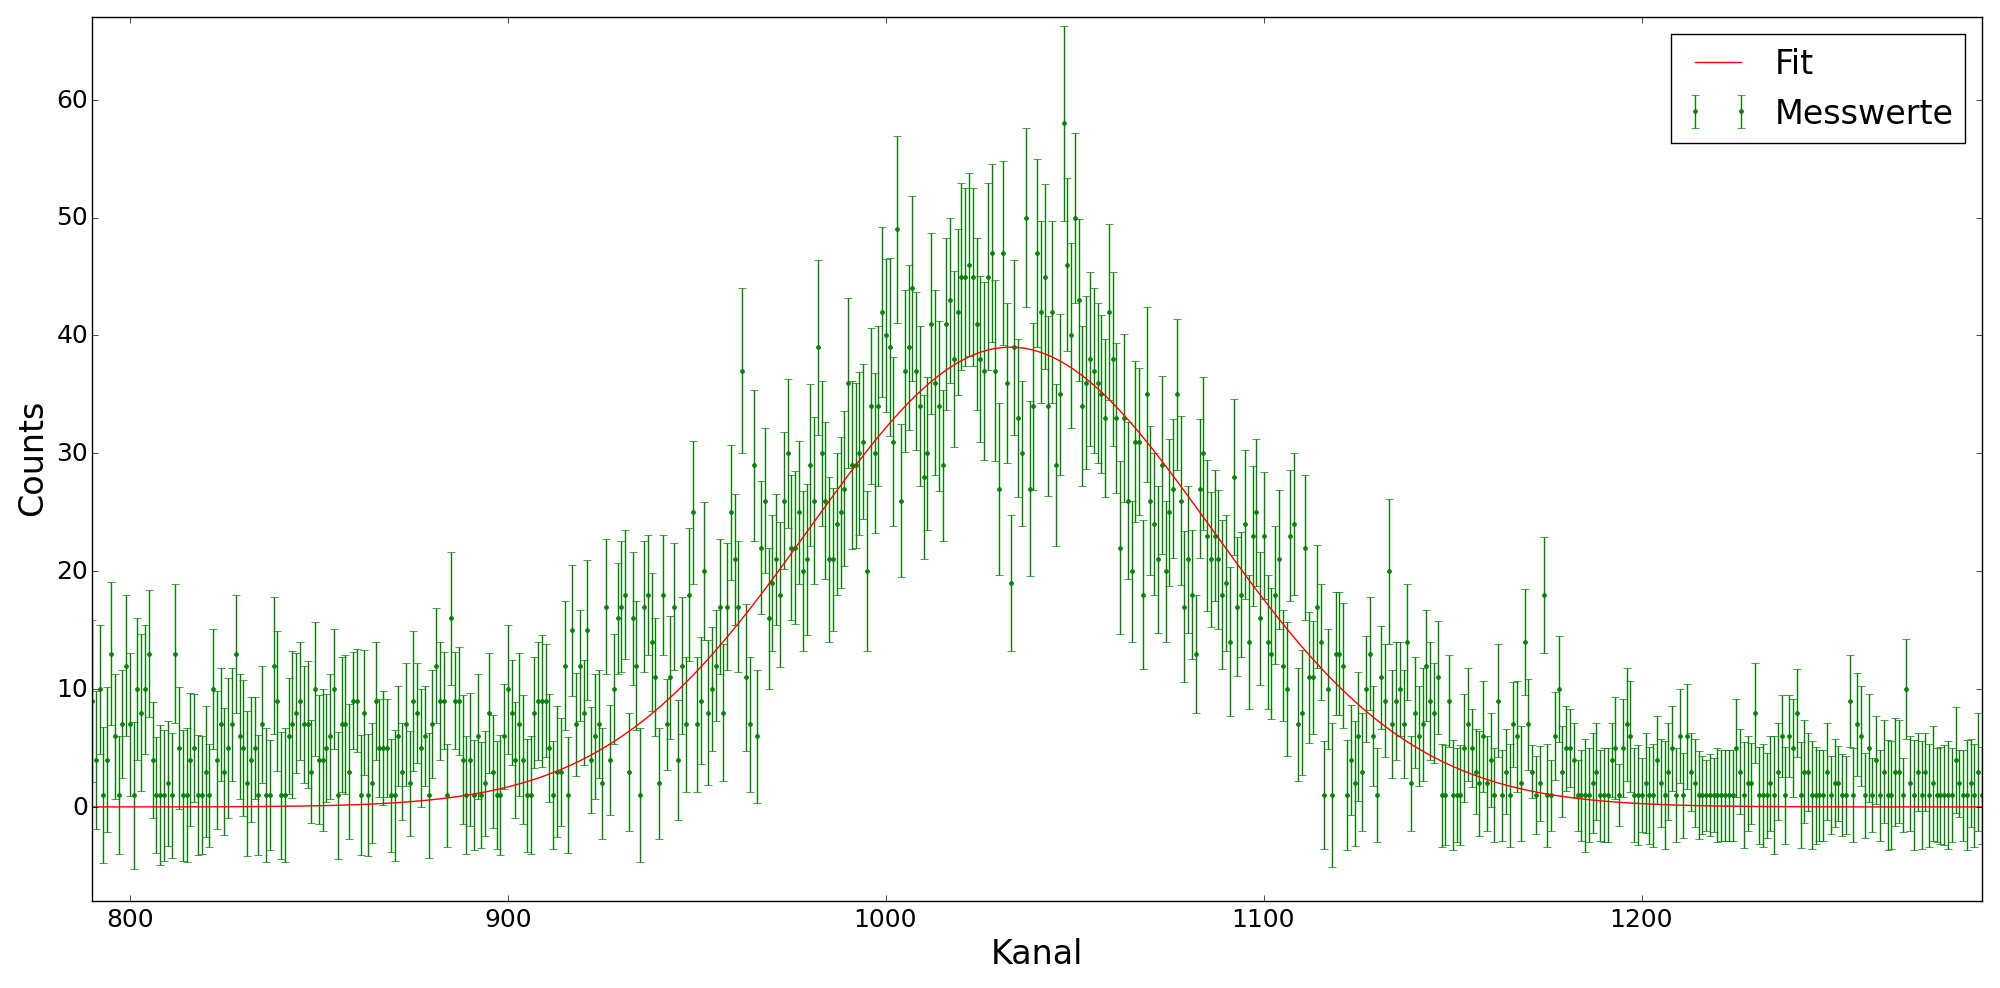
\includegraphics[scale = 0.34]{Wirkungsquerschnitt_80_Grad_Fit.png}
\caption{Die Fitparameter sind in Tabelle \ref{tab:80_Grad_WQ} eingetragen.}
\label{fig:Wirkungsquerschnitt_80}
\end{figure}

\begin{table}[H]
\centering
\caption{Fitparameter f�r die Energiemessung bei \SI{80}{\degree}. Das $\chi^2_{red}$ ergab sich mit 1.019}
\label{tab:80_Grad_WQ}
\begin{tabular}{|c|c|c|}
\hline Gau�peak & Parameter & Wert \\ 
\hline 1 & Amplitude & 5509(105) \\ 
\hline  & Center & 1027.8(14) \\ 
\hline  & Sigma & 60(3) \\ 
\hline 
\end{tabular} 
\end{table}

\printbibliography

\end{document}